\documentclass[]{article}

\usepackage{graphicx, caption}
\usepackage{placeins}
\usepackage{subfigure} 
\usepackage{float}

\topmargin 0.0cm
\oddsidemargin 0.2cm
\textwidth 16cm 
\textheight 21cm
\footskip 1.0cm
\usepackage{times}


%opening
\title{A simple {\it Science\/} Template} 
\author
{John Smith,$^{1\ast}$ Jane Doe,$^{1}$ Joe Scientist$^{2}$\\
	\\
	\normalsize{$^{1}$Department of Chemistry, University of Wherever,}\\
	\normalsize{An Unknown Address, Wherever, ST 00000, USA}\\
	\normalsize{$^{2}$Another Unknown Address, Palookaville, ST 99999, USA}\\
	\\
	\normalsize{$^\ast$To whom correspondence should be addressed; E-mail:  jsmith@wherever.edu.}
}

\date{\today}

\begin{document}
	
\baselineskip24pt

\maketitle

\begin{abstract}
 ** Things to be edited:
 Remove any language associating a country's ownership of a variant. It comes off as accusatory. 
 Change Dade figures to Miami-Dade and change South Africa to B.1.351
  Maybe save any conclusive commentary for the conclusion. Leave the paragraphs after each section as pure 'results' analysis
  Holiday/Fatalities missing dallas and houston
 
\end{abstract}

\indent Introduction. Explain why the study was necessary and explain what we looked at. 

\section*{COVID-19 variants and the daily case count}


\begin{figure}[!h]
	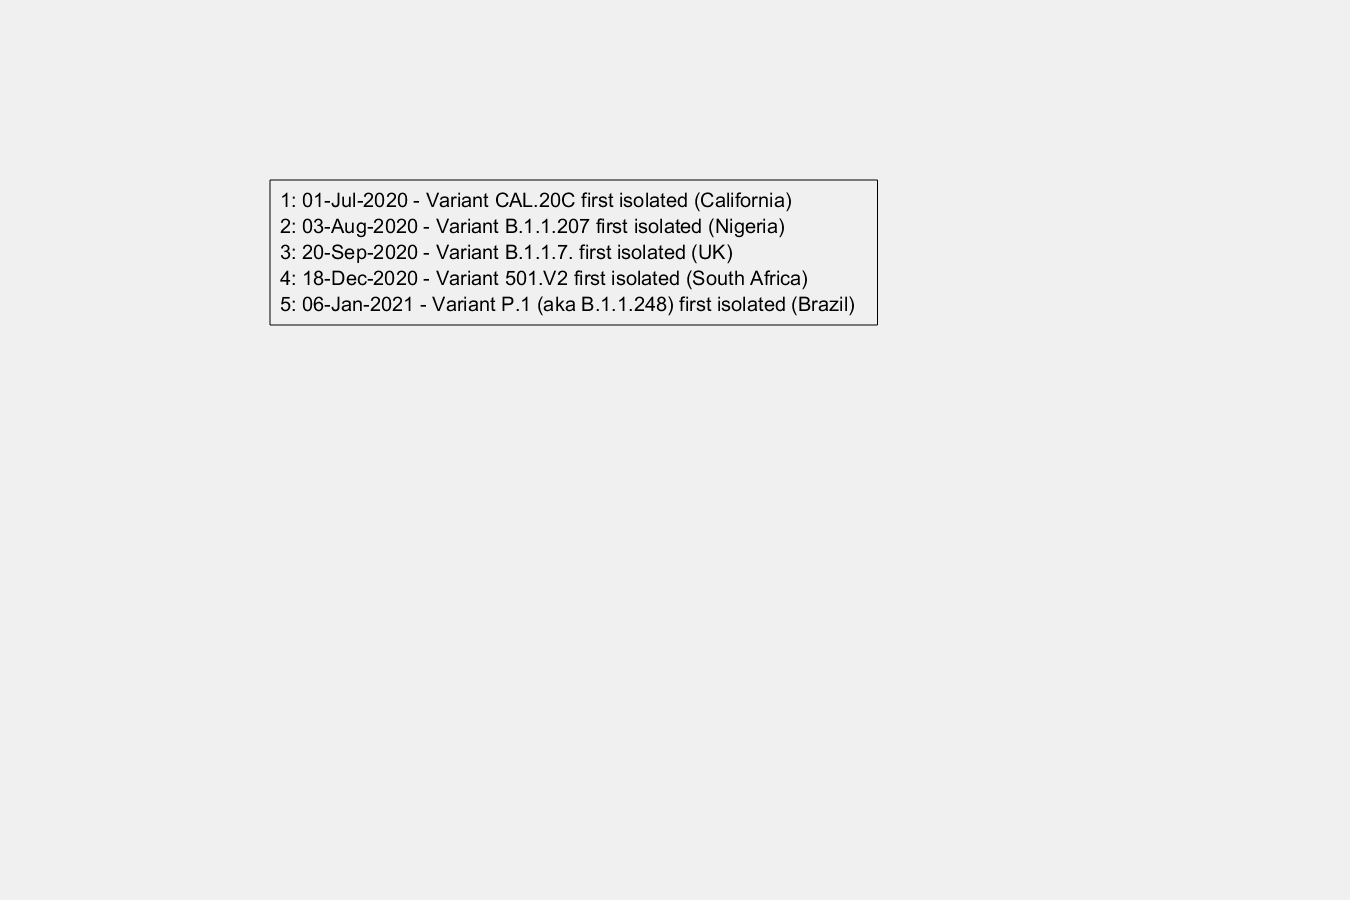
\includegraphics[width=\linewidth]{legends/variant_strains_legend.png}
	\caption{Listed above are five uniquely infectious variant strains of COVID-19,  listed corresponding to the date in which they were first genetically sequenced and isolated in their respective region.   }
	\label{fig:legends/variant_strains_legendLabel}
\end{figure}

\begin{figure}[!h]
	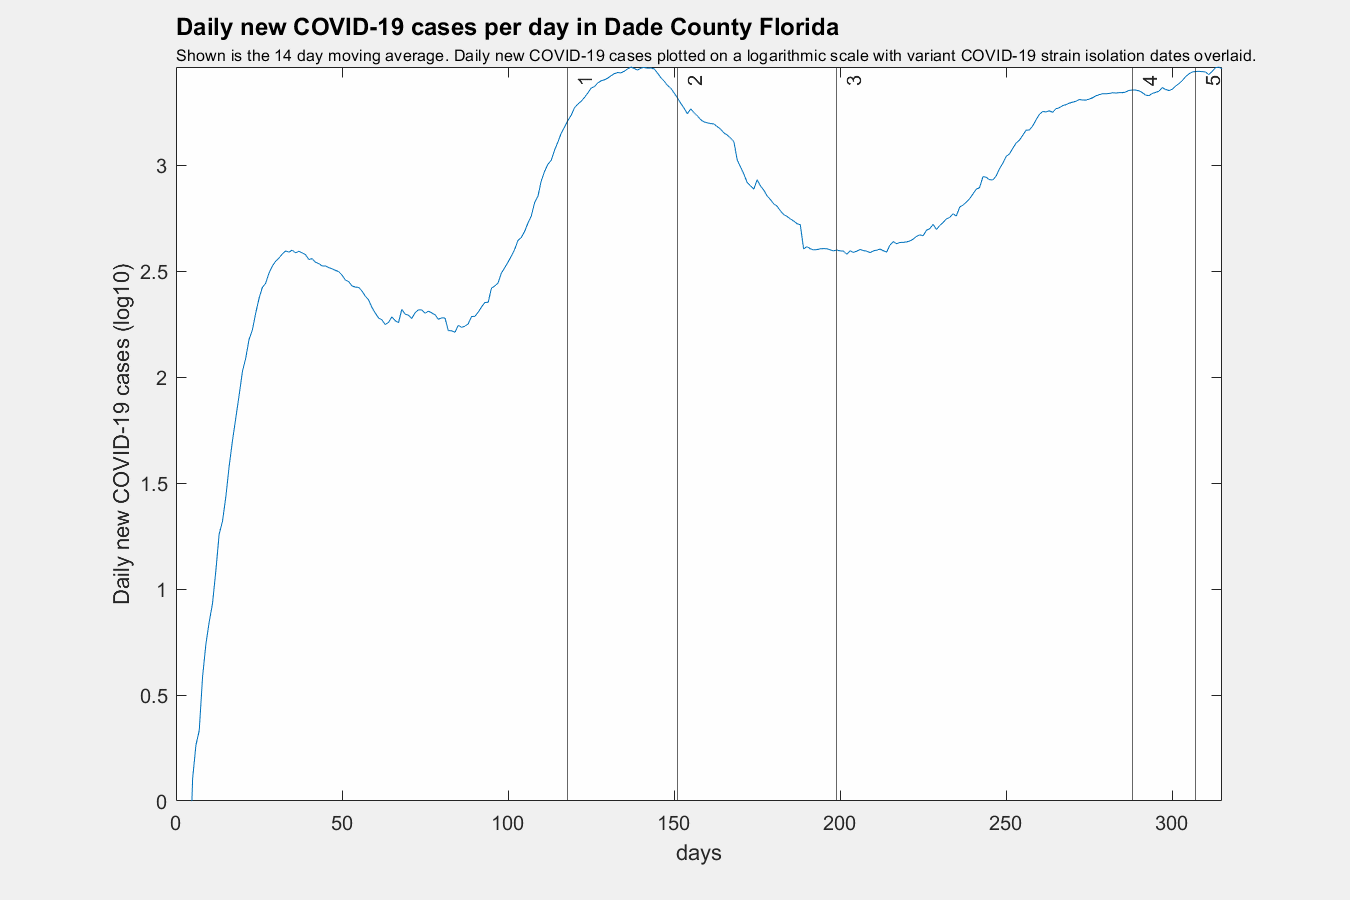
\includegraphics[width=\linewidth]{images/dade_cases_strains_log.png}
	\caption{Miami-Dade County Florida was already displaying it's steepest rate of daily new COVID-19 cases per day prior to the isolation of the California COVID-19 variant, CAL.20C (indicated in the figure as line 1). Dade County has yet to display a second climb as steep as the aforementioned local maximum; however, the rate of daily new COVID-19 cases per day in Dade County began to increase shortly after the UK variant COVID-19 strain, B.1.1.7, is isolated in the United Kingdom (indicated in the figurea as line 3).Since the isolation date of B.1.1.7, Dade County has yet to display indication of decrease in daily new COVID-19 cases per day. }
	\label{fig:images/dade_cases_strains_logLabel}
\end{figure}


\begin{figure}[!h]
	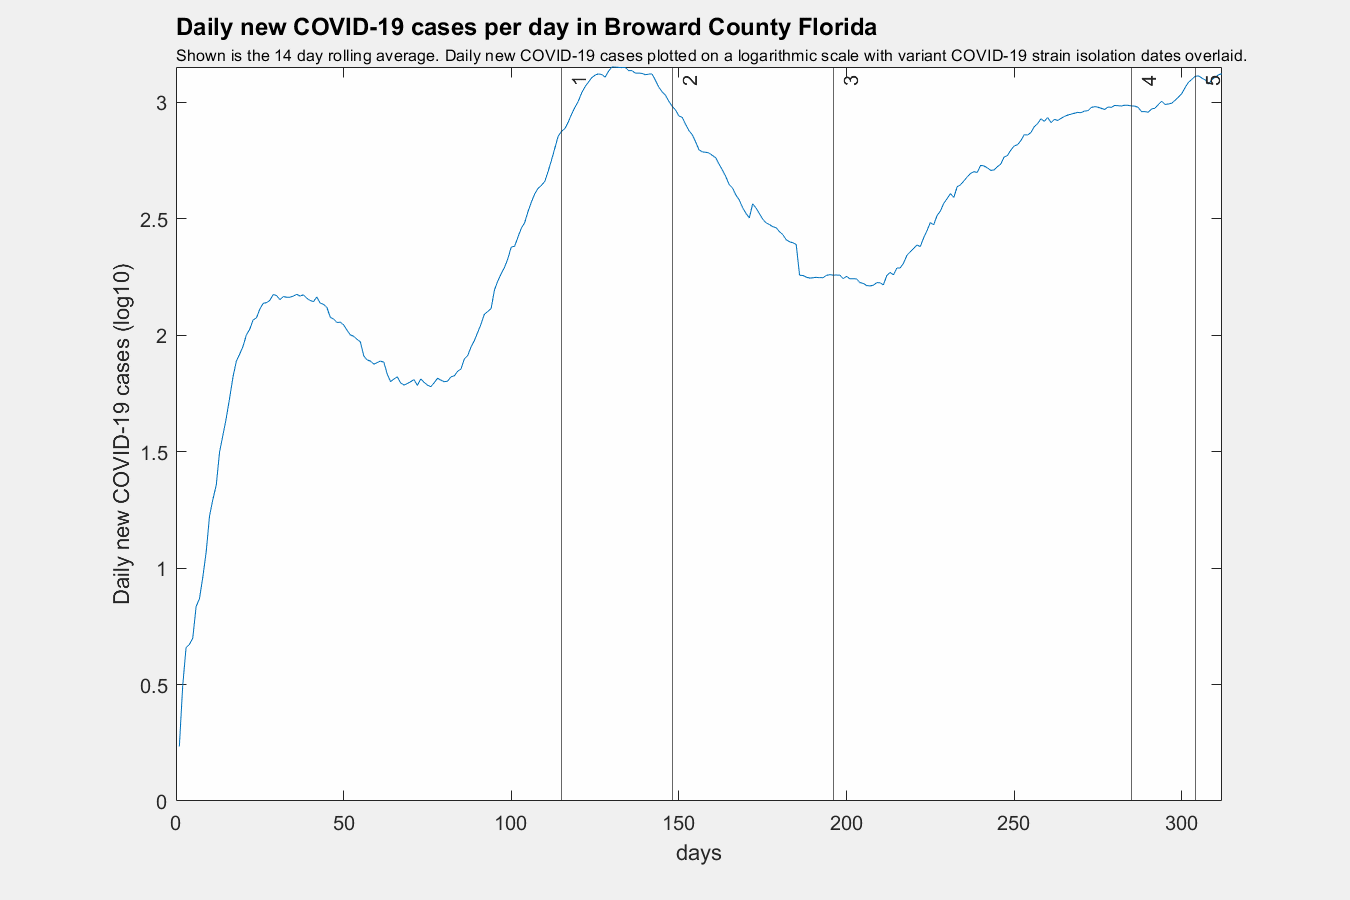
\includegraphics[width=\linewidth]{images/broward_cases_strains_log.png}
	\caption{In late July, Broward County Florida is displaying a global maximum in daily new COVID-19 cases per day, approximately two weeks after the COVID-19 variant strain, CAL.20C, is detected in California (indicated in the figure as line 1). After experiencing a moderate decline in daily new COVID-19 cases per day in early October, the rate of increase in daily new COVID-19 cases per day rises to a local maximum, offering no clear indication of decline. The aforementioned local maximum in daily new COVID-19 cases per day coincides with the detection date of the South African variant strain, B.1.351, and the Brazilian variant strain, P.1, (indicated in the figure as line 4 and 5) in their respective countries. }
	\label{fig:images/broward_cases_strains_logLabel}
\end{figure}


\begin{figure}[!h]
	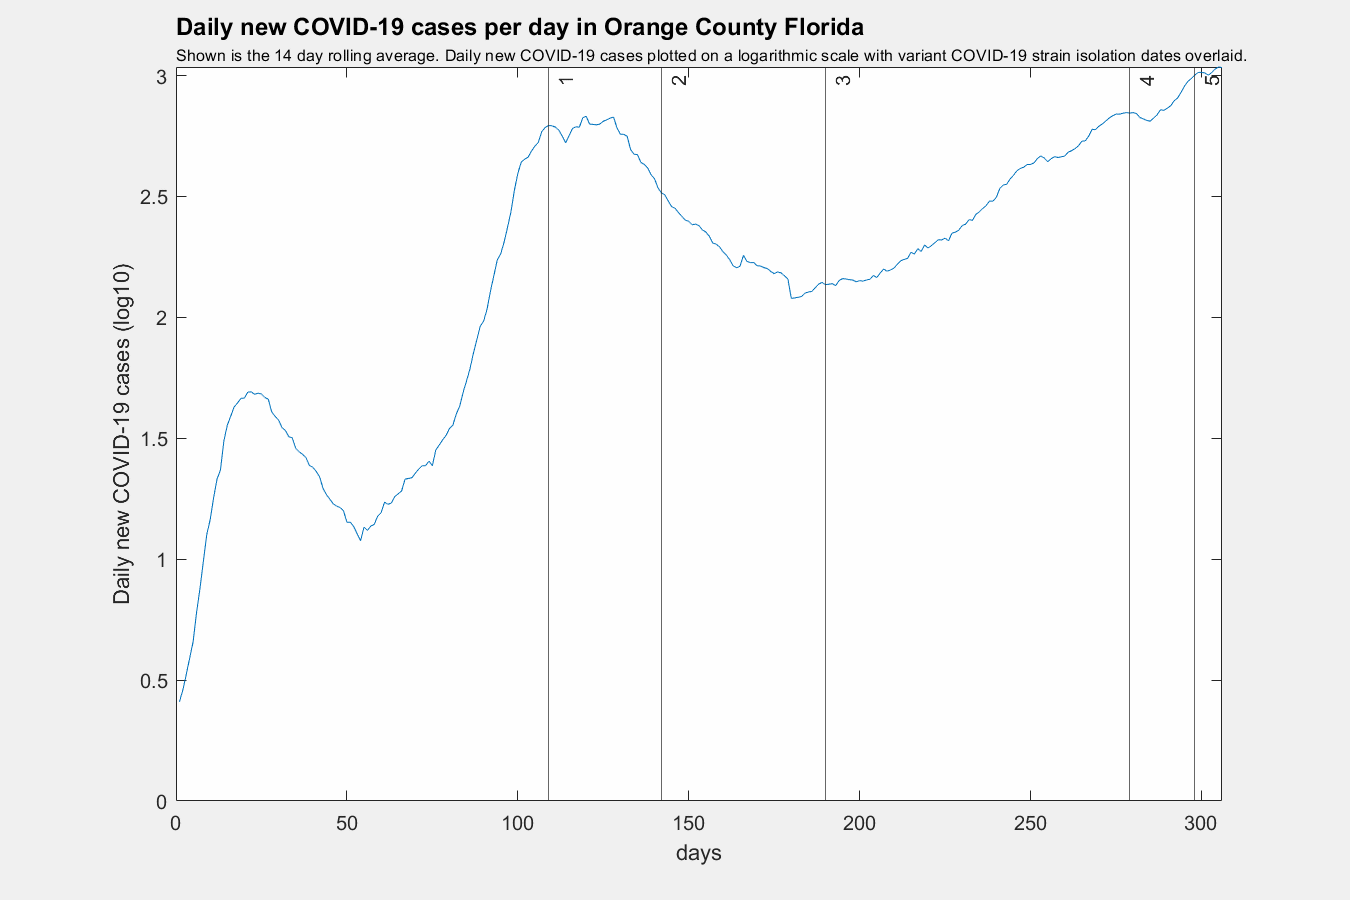
\includegraphics[width=\linewidth]{images/orange_cases_strains_log.png}
	\caption{Near mid July, daily new COVID-19 cases per day in Orange County Florida reach a local maximum, which arrives shortly after the California COVID-19 variant strain (indicated in the figure as line 1), CAL.20C, is first isolated in California. As the UK COVID-19 variant, B.1.1.7, is first sequenced in the United Kingdom (as indicated in the figure by line 3), Orange County is amidst an uphill trek in daily new COVID-19 cases per day.   }
	\label{fig:images/orange_cases_strains_logLabel}
\end{figure}

\begin{figure}[!h]
	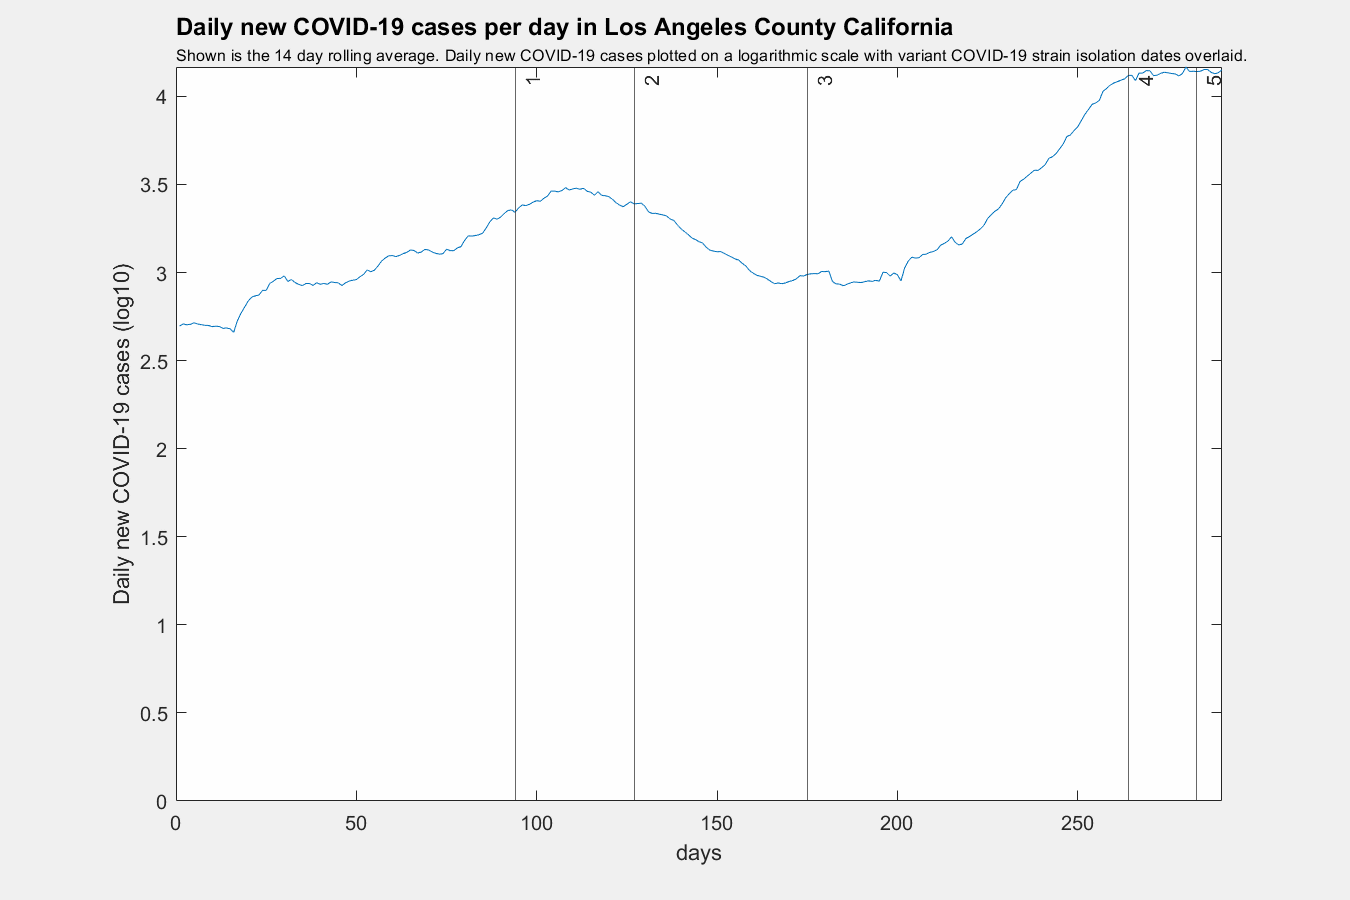
\includegraphics[width=\linewidth]{images/los_angeles_cases_strains_log.png}
	\caption{On July 1, 2020, the California COVID-19 variant, CAL.20C, is first isolated in California, indicated in the figure as line 1. At this time, daily new COVID-19 cases in Los Angeles County are approaching a local maximum in severity. Further, on September 20, 2020, 3 months after CAL.20C is first detected in Los Angeles county, the UK COVID-19 variant, B.1.1.7 (indicated in the figure as line 3), is first isolated in the UK, and daily new COVID-19 cases in Los Angeles County reach a global maximum after only briefly displaying a decline in daily new COVID-19 cases per day.  }
	\label{fig:images/los_angeles_cases_strains_logLabel}
\end{figure}


\begin{figure}[!h]
	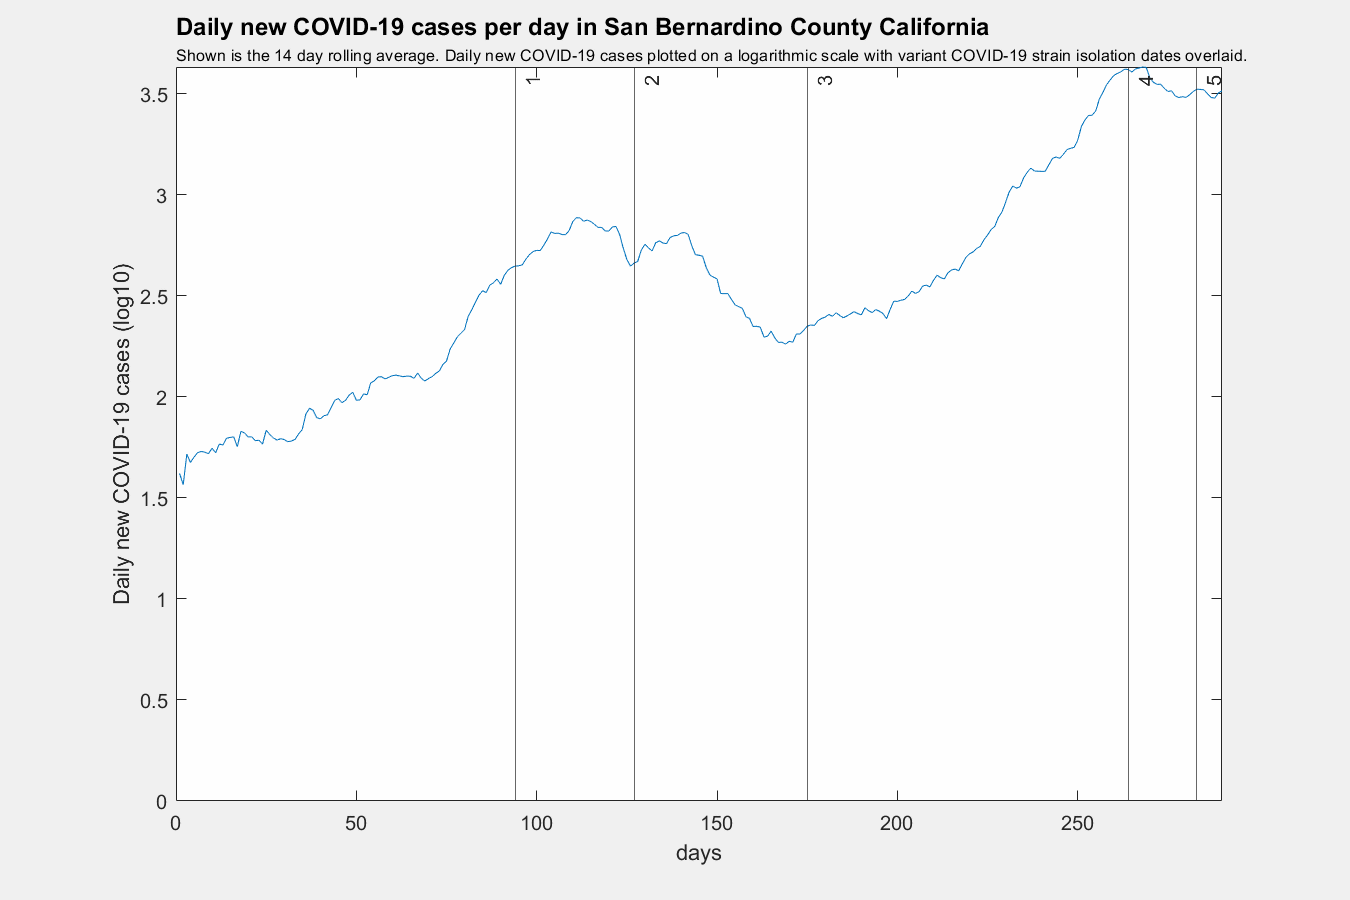
\includegraphics[width=\linewidth]{images/san_bernardino_cases_strains_log.png}
	\caption{On July 1,2020 , the California COVID-19 variant, CAL.20C, is first isolated in California (indicated in the figure as line 1), and San Bernardino County is in the process of reaching a local maximum in daily new COVID-19 cases per day. On September 20,2020 (indicated in the figure as line 3), the UK COVID-19 variant, B.1.1.7, is isolated in the UK, and simultaneously, daily new COVID-19 cases per day in San Bernardino County trek to a global maximum. }
	\label{fig:images/san_bernardino_cases_strains_logLabel}
\end{figure}


\begin{figure}[!h]
	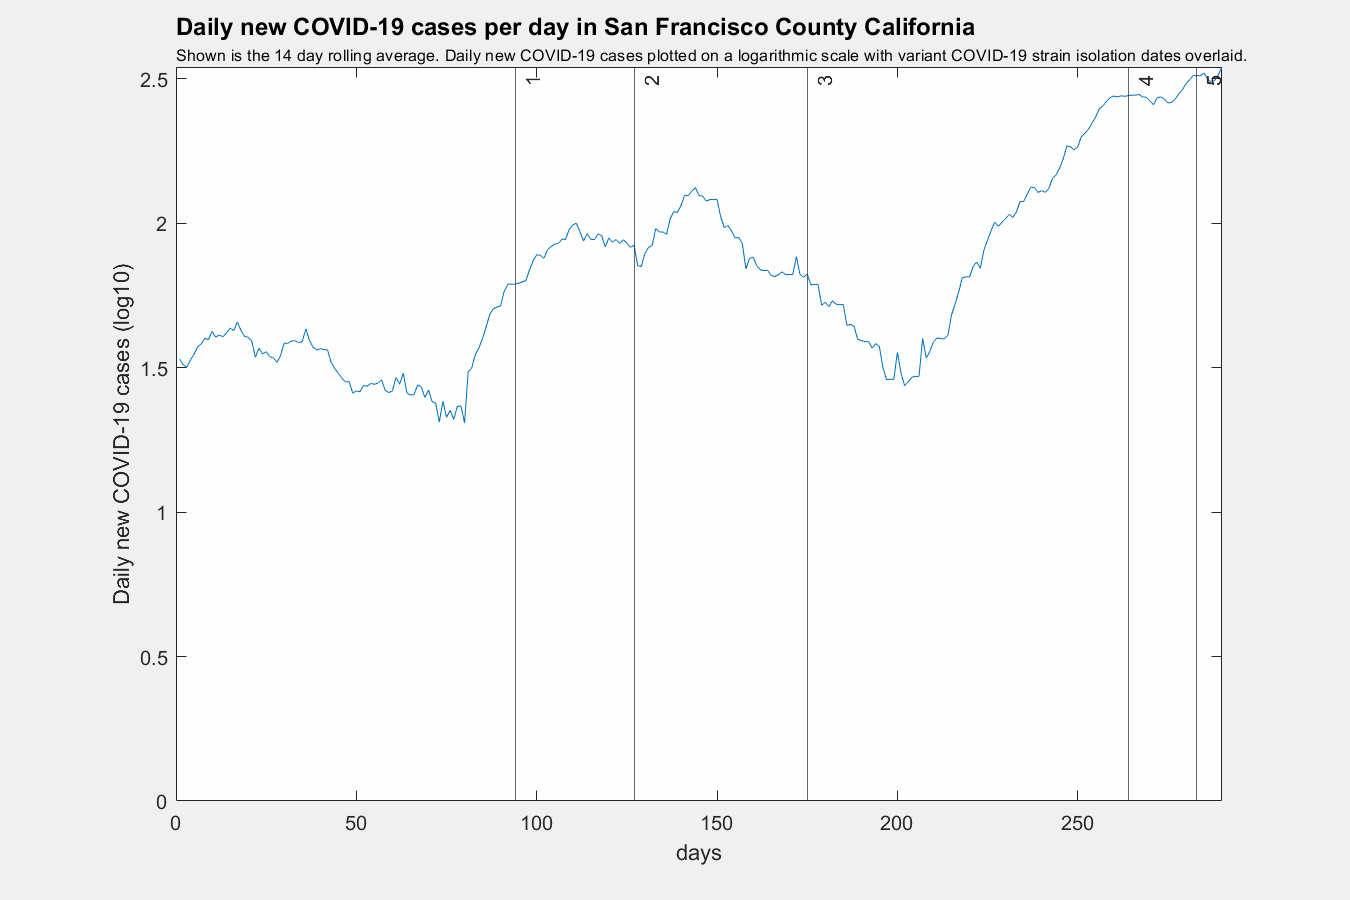
\includegraphics[width=\linewidth]{images/san_francisco_cases_strains_log.png}
	\caption{As the the California COVID-19 variant, CAL.20C, is first isolated in California (indicated in the figure as line 1), San Francisco County concludes it's steepest climb in daily new COVID-19 cases since the initiation of daily reporting. Approximately 50 days later, San Francisco County hits a local maximum in daily new COVID-19 cases per day. By mid December, San Francisco County reaches a global maximum in daily new COVID-19 cases per day, which coincides with the detection of the South African COVID-19 variant strain, B.1.351 and the Brazilian COVID-19 variant strain, P.1 (indicated in the figure as line 4 and 5).  }
	\label{fig:images/san_francisco_cases_strains_logLabel}
\end{figure}


\begin{figure}[!h]
	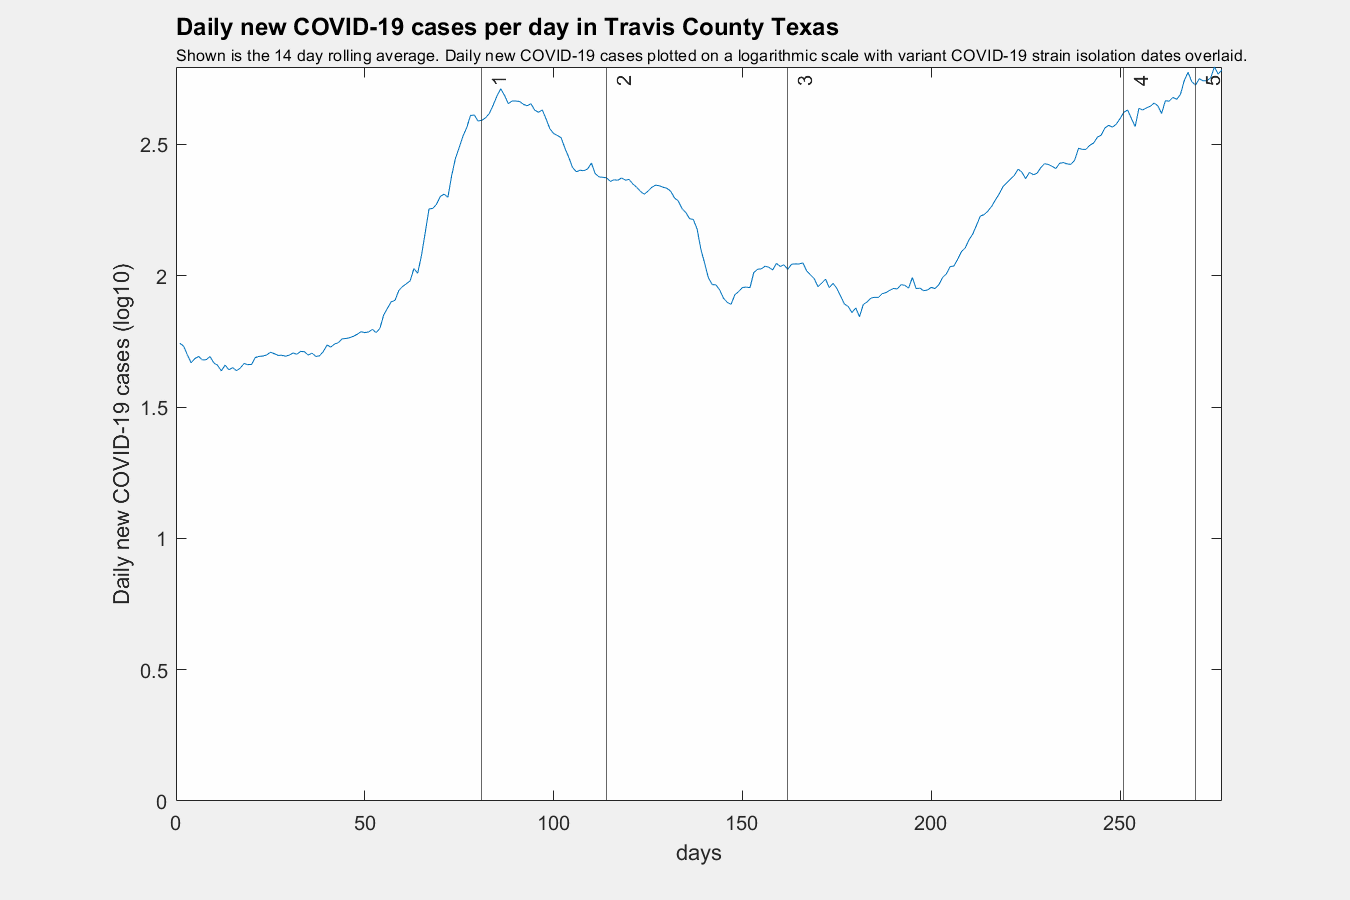
\includegraphics[width=\linewidth]{images/travis_cases_strains_log.png}
	\caption{On the day that the California COVID-19 variant, CAL.20C (indicated in the figure as line 1), is isolated, Travis County is just arriving at it's highest value of daily new COVID-19 cases per day since daily reporting of COVID-19 cases was initiated. When the UK variant, B.1.1.7 (indicated in the figure as line 3), was isolated in the United Kingdom, Travis county was displaying atop another local maximum, and headed for a great surge in the rate of daily new COVID-19 cases per day. }
	\label{fig:images/travis_cases_strains_logLabel}
\end{figure}

\begin{figure}[!h]
	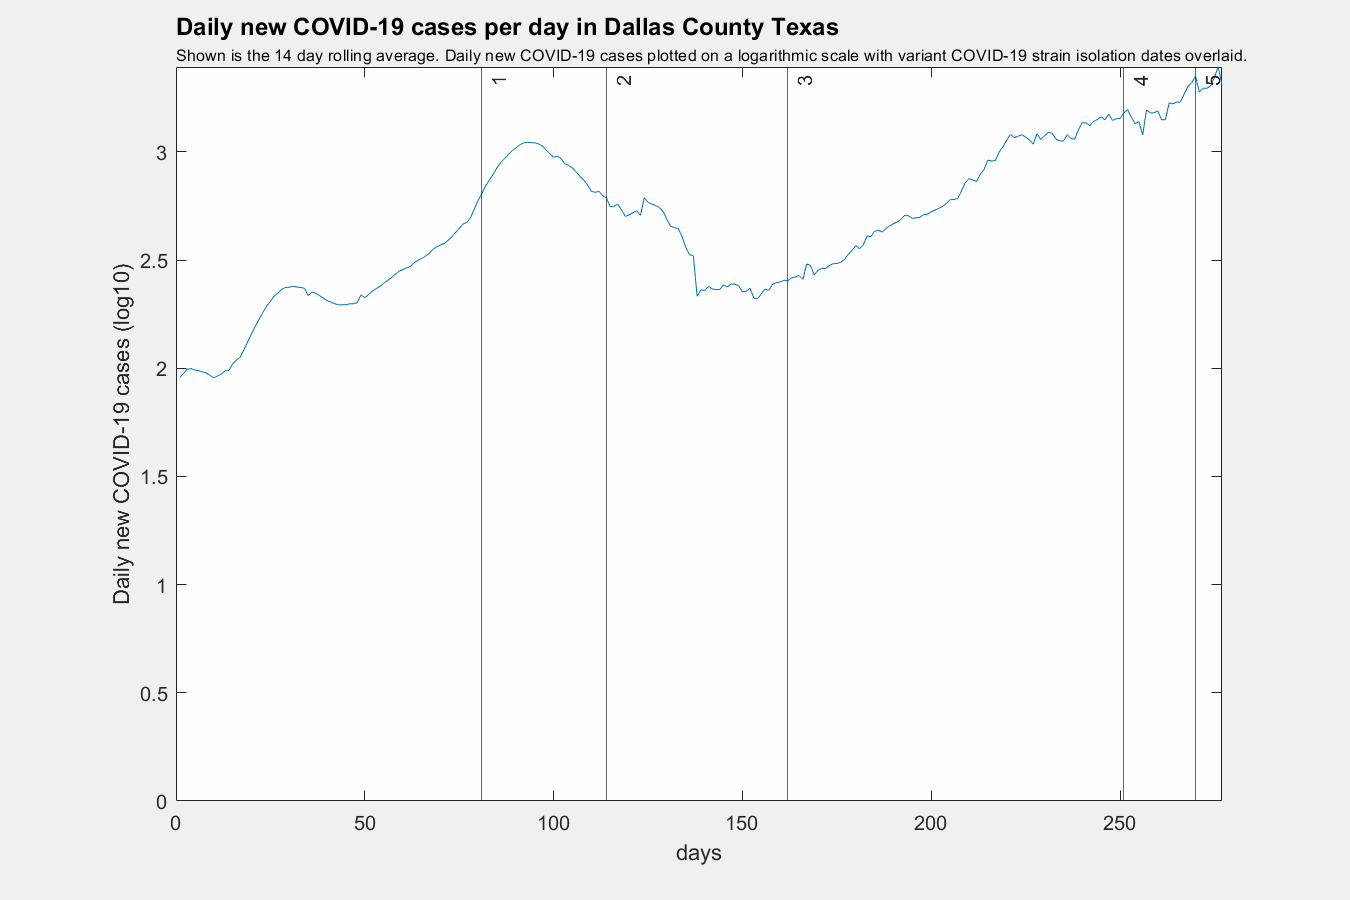
\includegraphics[width=\linewidth]{images/dallas_cases_strains_log.png}
	\caption{When the California COVID-19 variant, CAL.20C (indicated in the figure as line 1), is isolated, Dallas County is exhibiting a recent, new increase in the rate of daily new COVID-19 cases per day. A few weeks prior to the isolation date of the UK COVID-19 variant, B.1.1.7 (indicated in the figure as line 3), daily new COVID-19 cases in Dallas County began to steadily rise, resulting in consistently high recordings for daily new COVID-19 cases per day.   }
	\label{fig:images/dallas_cases_strains_logLabel}
\end{figure}

\begin{figure}[!h]
	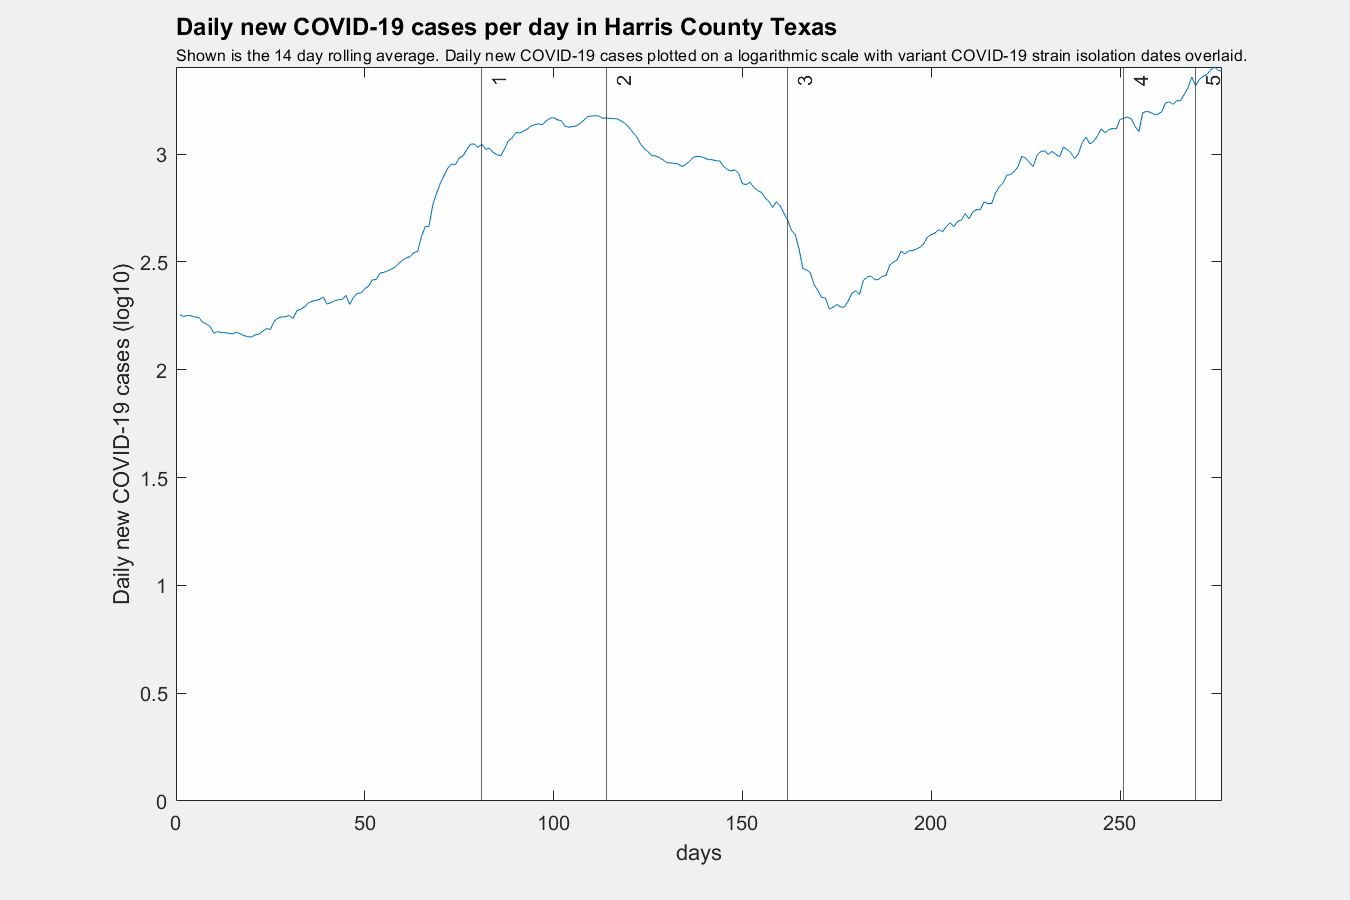
\includegraphics[width=\linewidth]{images/harris_cases_strains_log.png}
	\caption{When the COVID-19 variants from California, Nigeria and the United Kingdom (also known as CAL.20C, B.1.1.207, and B.1.1.7,as  indicated in the figure by line 1,2,and 3) are first genetically sequenced, Harris County is amidst a great local maximum in daily new COVID-19 cases being reported per day. Eventually, this maximum tapers off into a local minimum of daily reportings; however, approximately 10 days after the isolation of variant B.1.1.7., Harris County sees an steady increase in daily new COVID-19 cases per day.  }
	\label{fig:images/harris_cases_strains_logLabel}
\end{figure}


\FloatBarrier

\indent In figures 2-10, the 14 day moving average of daily new COVID-19 case count per day in 9 counties is displayed on a logarithmic scale ($log_{10}$) with vertical line overlays representing the dates when five sophisticated COVID-19 variant strains were first detected in their respective population. The counties assessed are Miami-Dade County, Florida; Broward County, Florida; Orange County, Florida; Los Angeles County, California; San Bernardino County, California; San Francisco County, California; Travis County, Texas; Dallas County, Texas; and Harris County, Texas. The genomic isolation dates of the COVID-19 variant strains in figures 2-10 are belonging to: CAL.20C (of lineage B.1.429), first isolated in California; B.1.1.207, first isolated in Nigeria; B.1.1.7 (aka VOC-202012/01, and as lineage B.1.1.7, or 20I/501Y.V1), first isolated in the United Kingdom; B.1.351 (aka 20H/501Y.V2, formerly known as 20C/501Y.V2), first isolated in South Africa; and P.1 (of lineage B.1.1.248), first isolated in Tokyo, and colloquially referred to as the Brazilian variant. 

 \indent Prior to the overlay of the first prominent COVID-19 variant displayed in each figure, 100\% of the counties are increasing in daily new COVID-19 cases per day. In 88.9\% of the counties, CAL.20C is overlayed an increasing slope representing the change in daily new COVID-19 cases per day. Specifically, San Francisco County in California, which was undergoing an exponential rate of change in daily new COVID-19 cases per day when CAL.20C was first detected. It's possible that CAL.20C may have been circulating in the population undetected for an unknown period of time prior to genomic sequencing.
 
 \indent After the Nigerian COVID-19 variant, B.1.1.207 is isolated, 66.7\% of the counties are displaying a steady decline in daily new COVID-19 cases per day, 11.1\% of the counties display a shallow local minimum in cases after the detection of variant B.1.1.207, and 22.2\% of the counties display an increase in daily new COVID-19 cases per day after the detection of B.1.1.207, followed by a decline in the rate of daily new COVID-19 cases per day. Due to the absence of a coherent response among the counties in regards to the isolation of the Nigerian COVID-19 variant, B.1.1.207, it's possible that this variant has had marginal impact on the rate of daily new COVID-19 cases per day in these respective counties.
 
 \indent When the isolation date of the UK COVID-19 variant, B.1.1.7, occurs, 55.6\% of the counties are experiencing a local minimum in daily new COVID-19 cases per day, 22.2\% of the counties are amidst a decline in daily new COVID-19 cases per day, 11.1\% of the counties are at a local maximum, and 11.1\% of the counties are at the base of a steep rise in daily new COVID-19 cases per day; however, 100\% of the counties display a perpetual increase in daily new COVID-19 cases per day either the day of, or shortly after the isolation date of the COVID-19 variant B.1.1.7.
 
 \indent The genomic isolation date of the South African variant, B.1.351, occurs just before the sequencing date of the Brazilian COVID-19 variant, P.1. As both variants are identified, 100\% of the counties are amidst their greatest daily reportings for daily new COVID-19 cases per day and 100\% of the counties continue reporting staggeringly high daily new COVID-19 cases per day. After the arrival of both B.1.351 and P.1. 100\% of the counties are reporting daily record-breaking values in new COVID-19 cases per day for their respective population. It's inconclusive as to the implication of B.1.351 and P.1 on the aforementioned counties, as 100\% of the counties are already experience a surge in daily new COVID-19 cases when B.1.351 and P.1 are identified. 
 
 
\FloatBarrier
\vspace{5mm}
\section*{COVID-19 variants and daily new hospitalizations}

\begin{figure}[!h]
	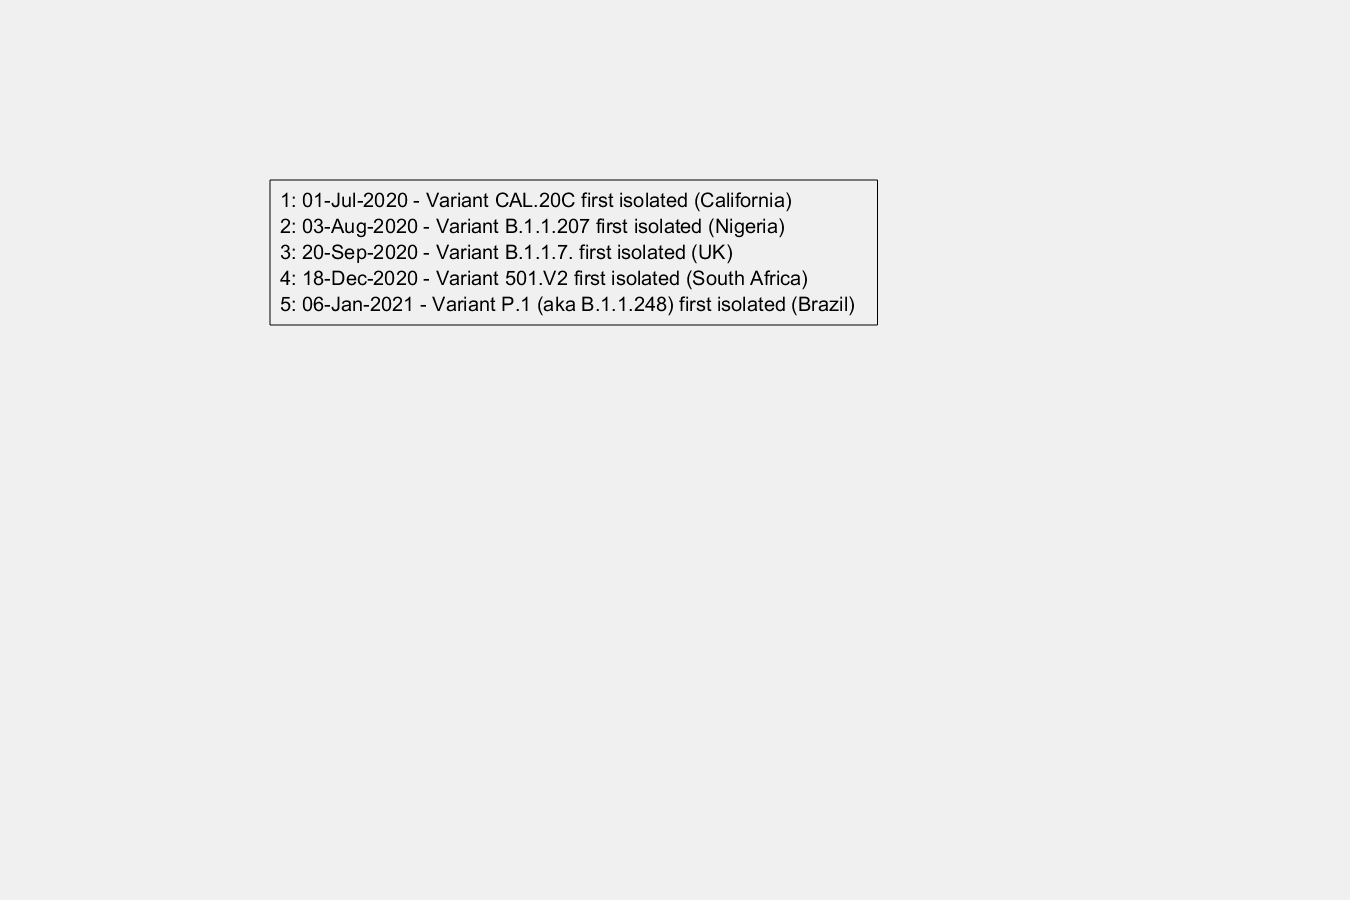
\includegraphics[width=\linewidth]{legends/variant_strains_legend.png}
	\caption{Listed above are five uniquely infectious variant strains of COVID-19,  listed corresponding to the date in which they were first genetically sequenced and isolated in their respective region.}
	\label{fig:legends/variant_strains_legendLabel}
\end{figure}

\begin{figure}[!h]
	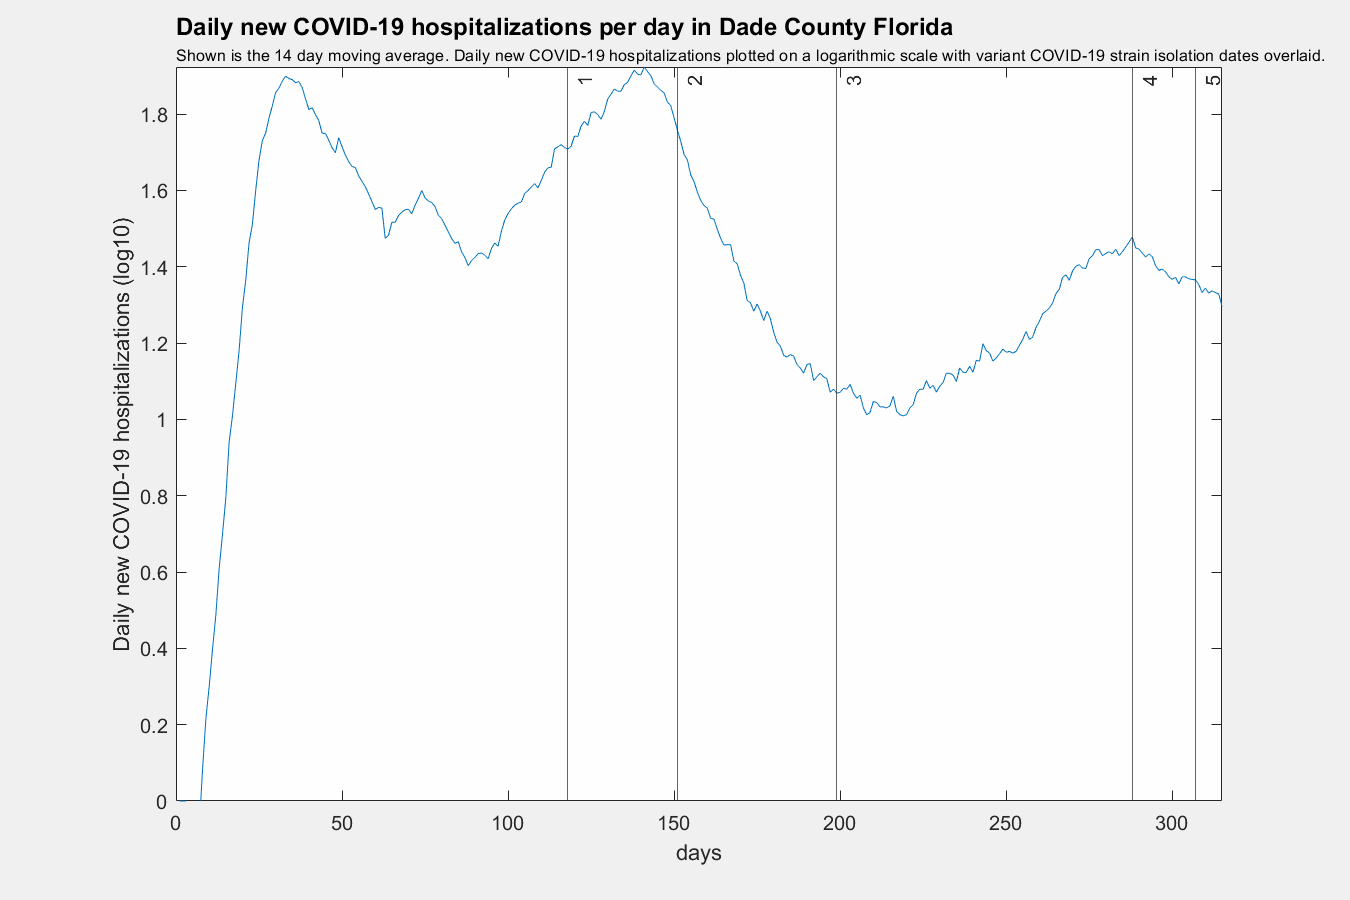
\includegraphics[width=\linewidth]{images/dade_hospitalizations_strains_log.png}
	\caption{Overall, daily new COVID-19 hospitalizations in Miami-Dade County have decreased since the start of daily COVID-19 reportings. After the isolation date of the California variant, CAL.20C (indicated in the figure as line 1), Miami-Dade County reaches a local maximum, matching their previous record for the highest value in daily new COVID-19 cases reported in a single day. Shortly after their second local maximum in dailyCOVID-19 hospitalizations, Miami-Dade County undergoes a dramatic decline in hospitalizations. However, when the UK COVID-19 variant, B.1.1.7 (indicated in the figure as line 3), is isolated, the daily new COVID-19 hospitalization curve for Miami-Dade County begins to turn, and rise for a third time.     }
	\label{fig:images/dade_hospitalizations_strains_logLabel}
\end{figure}


\begin{figure}[!h]
	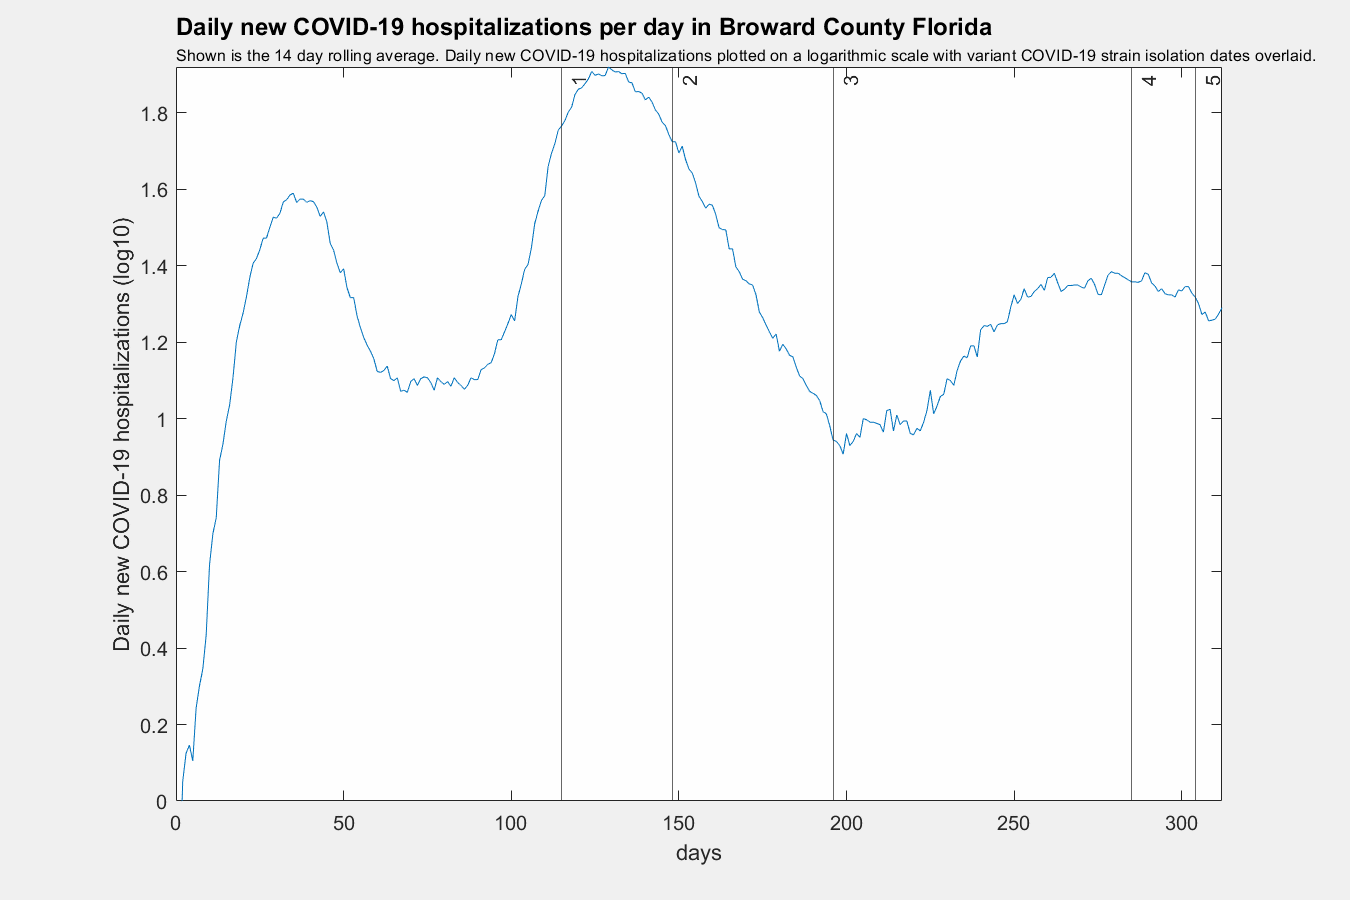
\includegraphics[width=\linewidth]{images/broward_hospitalizations_strains_log.png}
	\caption{As the California COVID-19 variant, CAL.20C (indicated in the figure as line 1), is first isolated, Broward County is nearing the peak of it's highest set of daily new COVID-19 hospitalizations since daily COVID-19 reporting began. Since the aformentioned global maximum in daily new COVDI-19 hospitalizations, Broward County has yet to experience daily hospitalizations at that level. However, shortly after the isolation date of the UK COVID-19 variant, B.1.1.7 (indicated in the figure as line 3), daily new COVID-19 hospitalizations in Broward County rises for a third time.  }
	\label{fig:images/broward_hospitalizations_strains_logLabel}
\end{figure}


\begin{figure}[!h]
	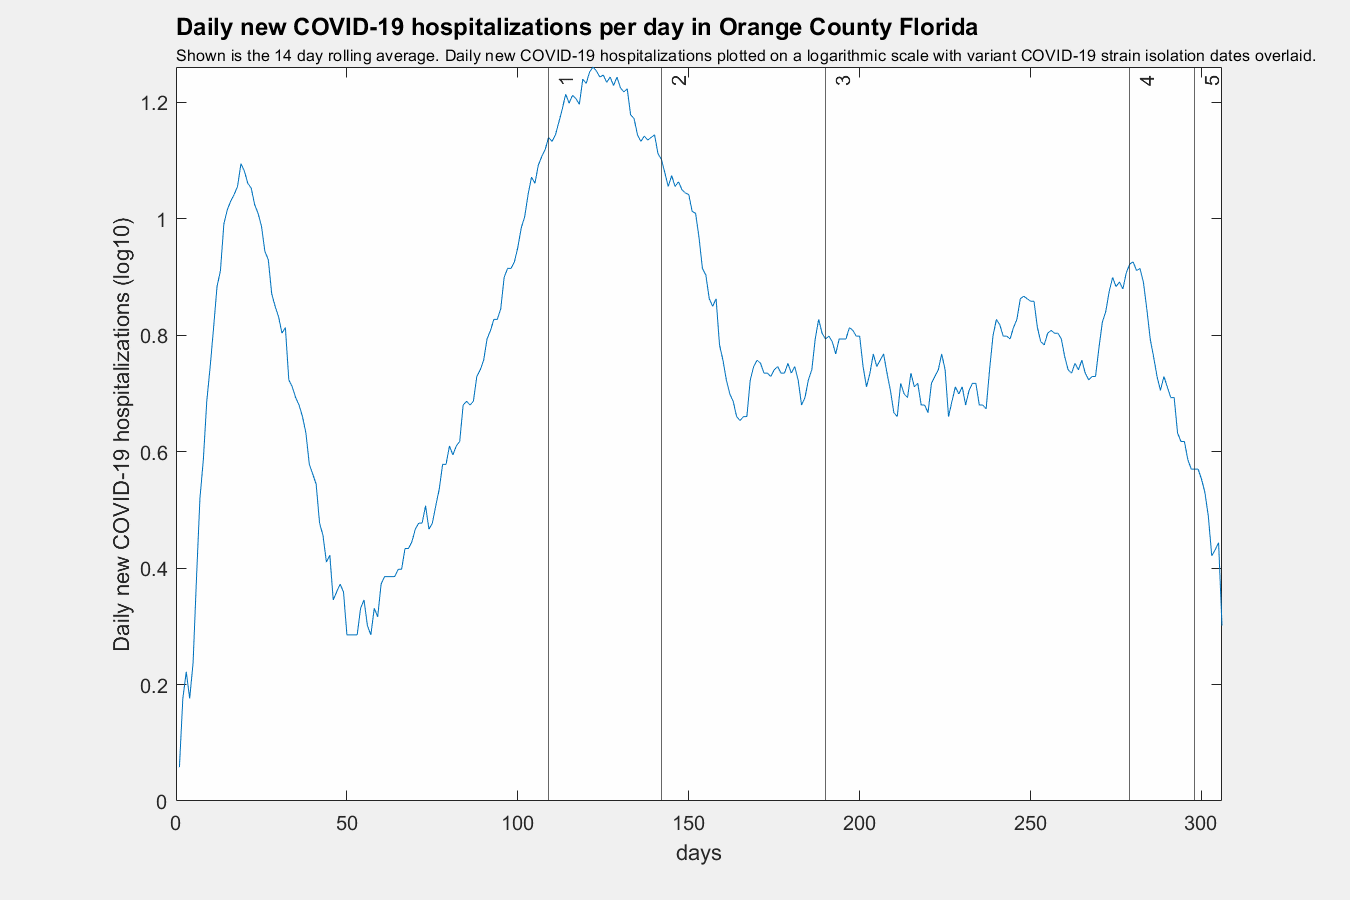
\includegraphics[width=\linewidth]{images/orange_hospitalizations_strains_log.png}
	\caption{After Orange County's first surge in daily new COVID-19 hospitalizations per day, they experience an immediate second wave of of higher magnitude. The peak of the second wave coincides with the isolation date of the California COVID-19 variant, CAL.20C (indicated in the figure as line 1). After the second wave of daily new COVID-19 hospitalizations, hospitaliations in Orange County maintain relatively stable.}
	\label{fig:images/orange_hospitalizations_strains_logLabel}
\end{figure}


\begin{figure}[!h]
	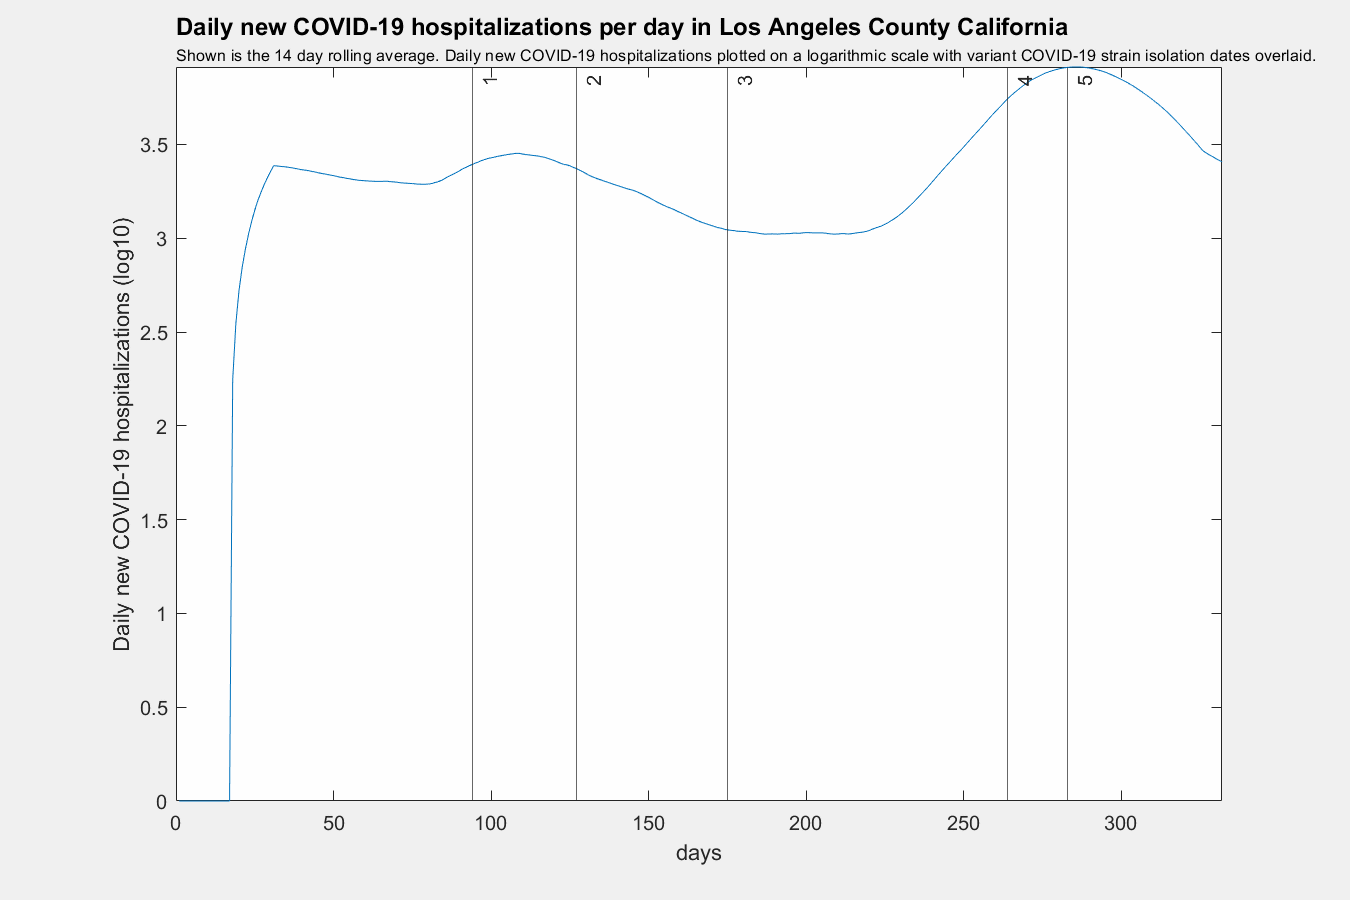
\includegraphics[width=\linewidth]{images/los_angeles_hospitalizations_strains_log.png}
	\caption{The rate of daily new COVID-19 hospitalizations in Los Angeles County has been constant for most of the reporting period. Los Angeles County experienced a mild increase in daily new COVID-19 cases during the isolation of varint CAL.20C (indicated in the figurea as line 1), but the rate began to drop shortly after. At the time when the South African variant, B.1.351 (line 4 in the figure), and Brazilian variant, P.1 (line 5 in the figure), are isolated, Los Angeles County is amidst a dramatic surge in daily new COVID-19 hospitalizations per day.}
	\label{fig:images/los_angeles_hospitalizations_strains_logLabel}
\end{figure}


\begin{figure}[!h]
	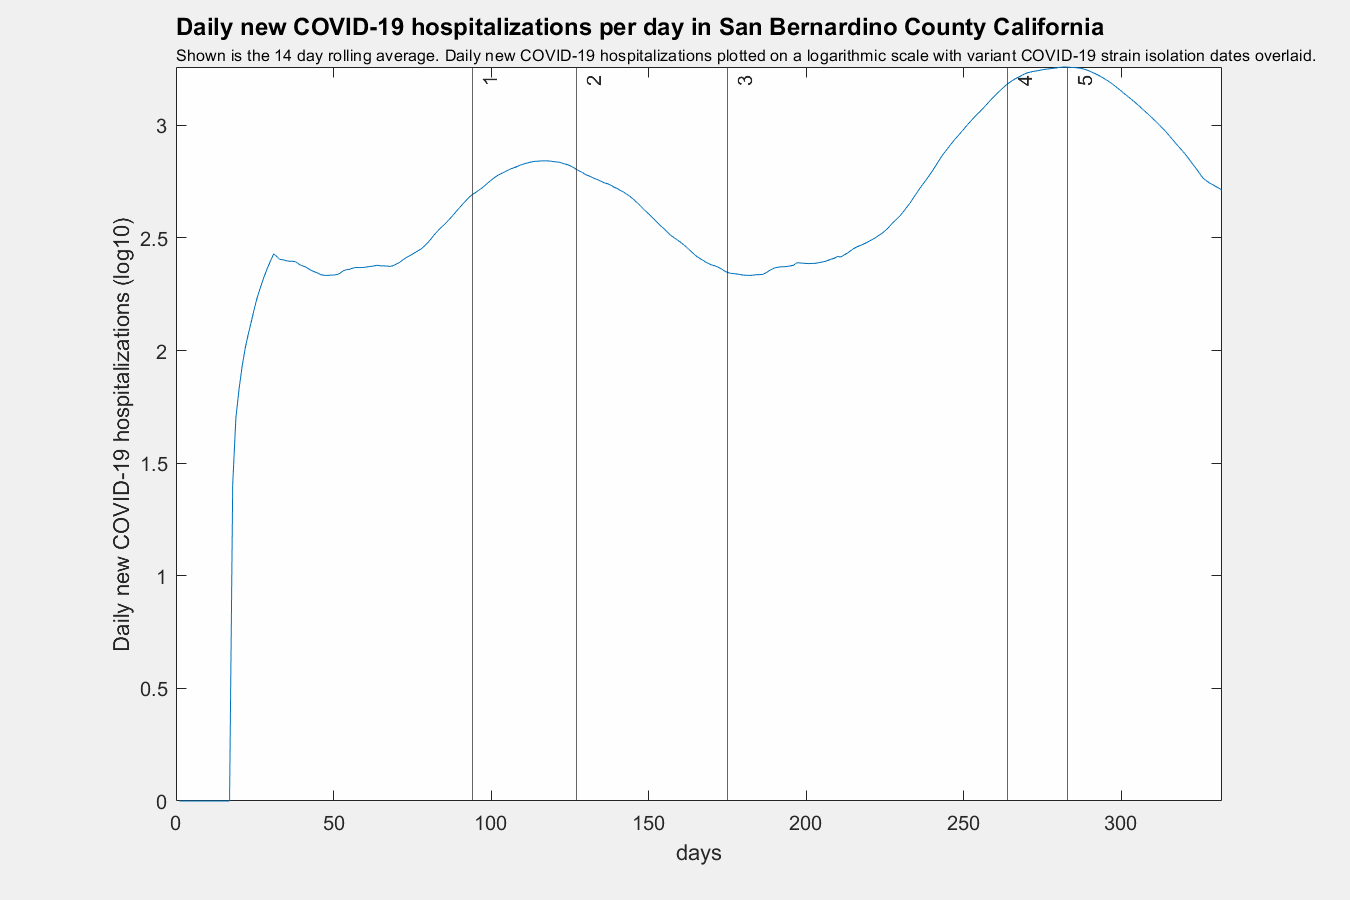
\includegraphics[width=\linewidth]{images/san_bernardino_hospitalizations_strains_log.png}
	\caption{Shortly after San Bernardino experiences it's first local maximum in daily new COVID-19 cases, the California variant, CAL.20C (indicated in the figure as line 1), is isolated. When the UK variant, B.1.1.7 (indicated in the figure as line 3), is first isolated, San Bernardino is experiencing a local minimum in daily hospitalization reportings; however, shortly thereafter, the rate in daily new COVID-19 cases per day begins to climb. }
	\label{fig:images/san_bernardino_hospitalizations_strains_logLabel}
\end{figure}


\begin{figure}[!h]
	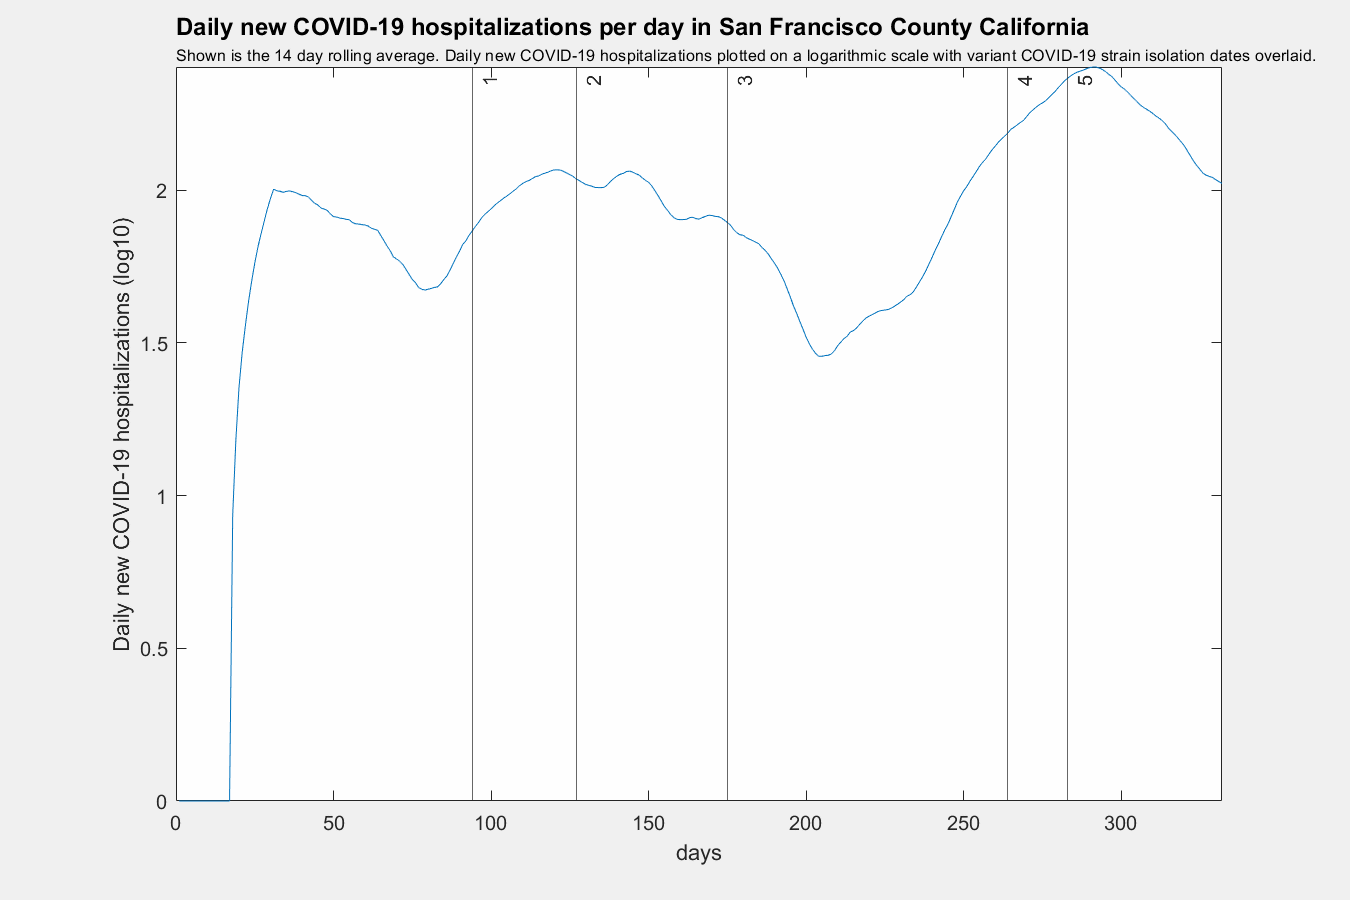
\includegraphics[width=\linewidth]{images/san_francisco_hospitalizations_strains_log.png}
	\caption{In San Francisco County, daily new COVID-19 hospitalizations are at a local maximum when CAL.20C, B.1.1.207, and B.1.1.7 (indicated in the figure as line 1, 2, and 3) are first genetically isolated. After the isolation date of the UK COVID-19 variant, B.1.1.7, San Francisco County drops in daily new COVID-19 hospitalizations per day; however, soon thereafter, the rate begins to increase on an uphill trend, without indication of decrease.  }
	\label{fig:images/san_francisco_hospitalizations_strains_logLabel}
\end{figure}

\begin{figure}[!h]
	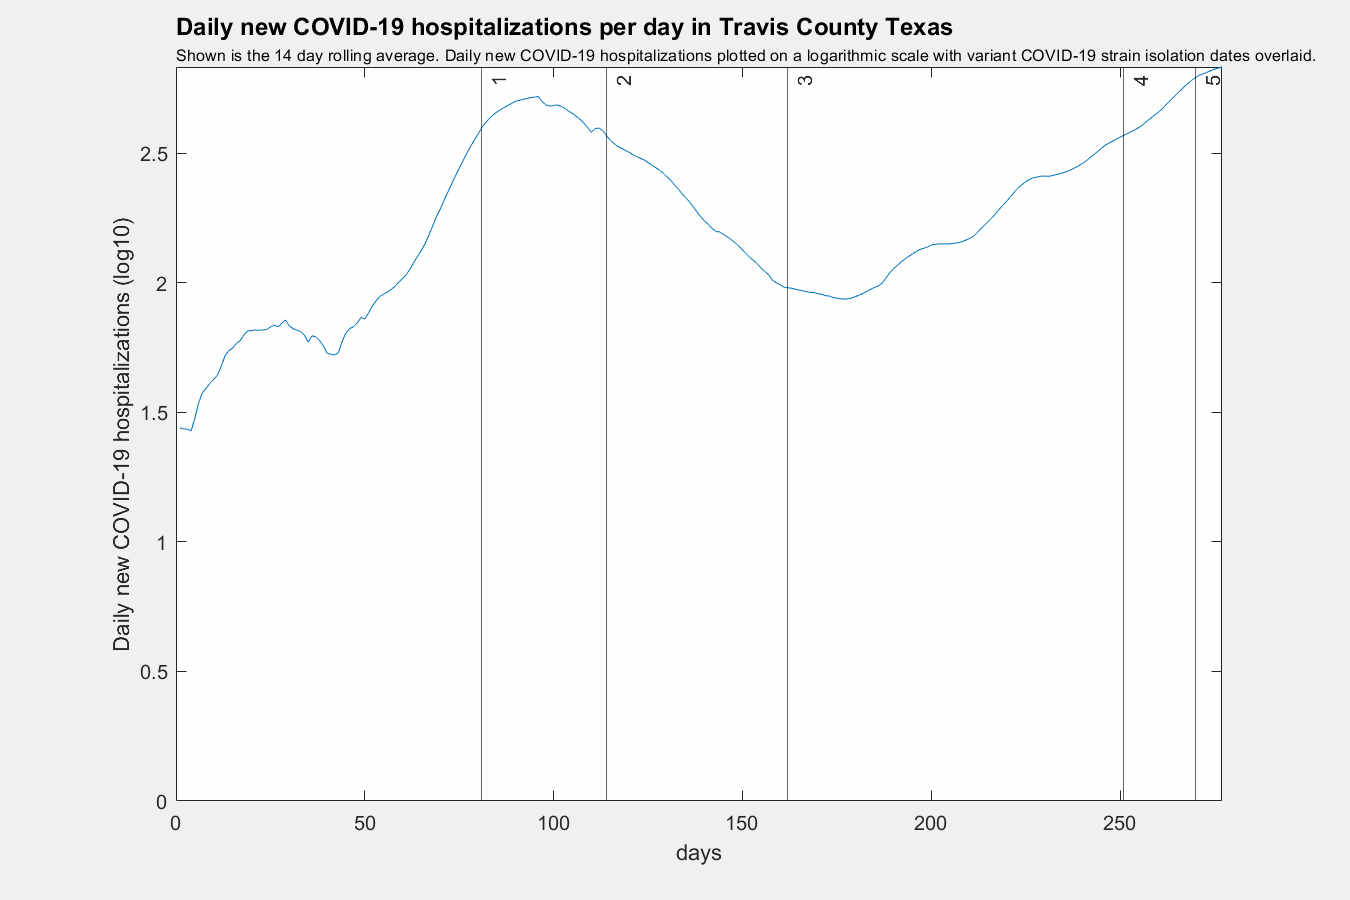
\includegraphics[width=\linewidth]{images/travis_hospitalizations_strains_log.png}
	\caption{Daily new COVID-19 hospitalizations per day in Travis County are trending towards their first local maximum as daily reporting is initiated. When the COVID-19 variant CAL.20C (indicated in the figure as line 1) is first isolated, Travis County is nearing the peak of a second, much higher local maximum in daily new COVID-19 hospitalizations. As this second peak is dropping, the UK COVID-19 variant, B.1.1.7 (indicated in the figure as line 3), is isolated, whereby daily new COVID-19 hospitalizations per day in Travis County begin to rise again.  }
	\label{fig:images/travis_hospitalizations_strains_logLabel}
\end{figure}

\begin{figure}[!h]
	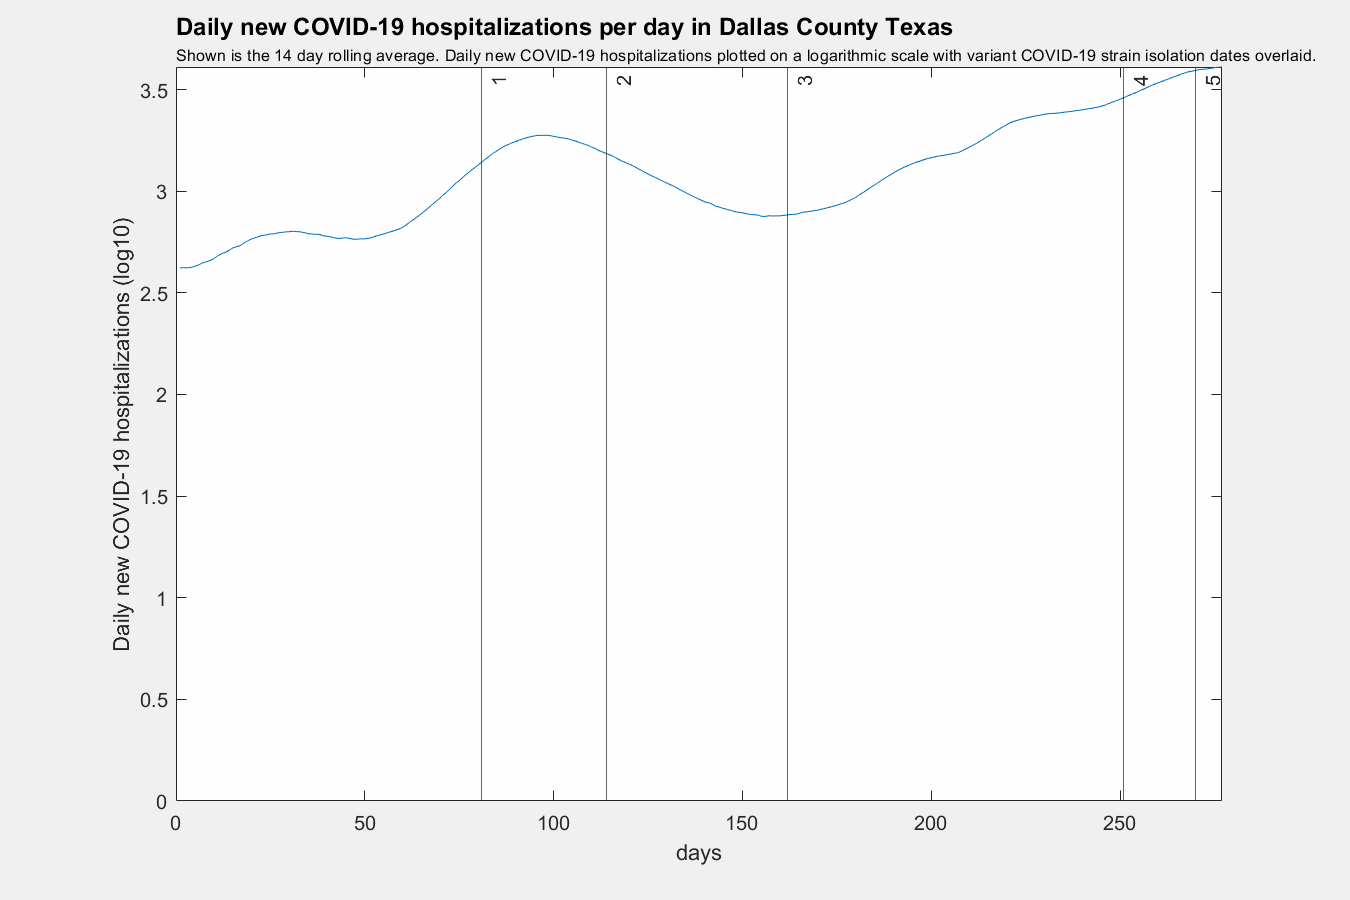
\includegraphics[width=\linewidth]{images/dallas_hospitalizations_strains_log.png}
	\caption{Daily new COVID-19 hospitalizations per day in Dallas County have been steadily increasing since the initiation of daily reporting. When the California COVID-19 variant, CAL.20C (indicated in the figure as line 1), was first isolated, Dallas County was displaying a local maximum in daily new COVID-19 hospitalizations per day. Shortly after this local maximum, daily new hospitalizations began to decline. At the time when the UK COVID-19 variant, B.1.1.7 (indicated in the figure as line 3), is genetically isolated, Dallas County begins to rise in daily new COVID-19 hospitalizations per day without any apparent sign in decrease.  }
	\label{fig:images/dallas_hospitalizations_strains_logLabel}
\end{figure}

\begin{figure}[!h]
	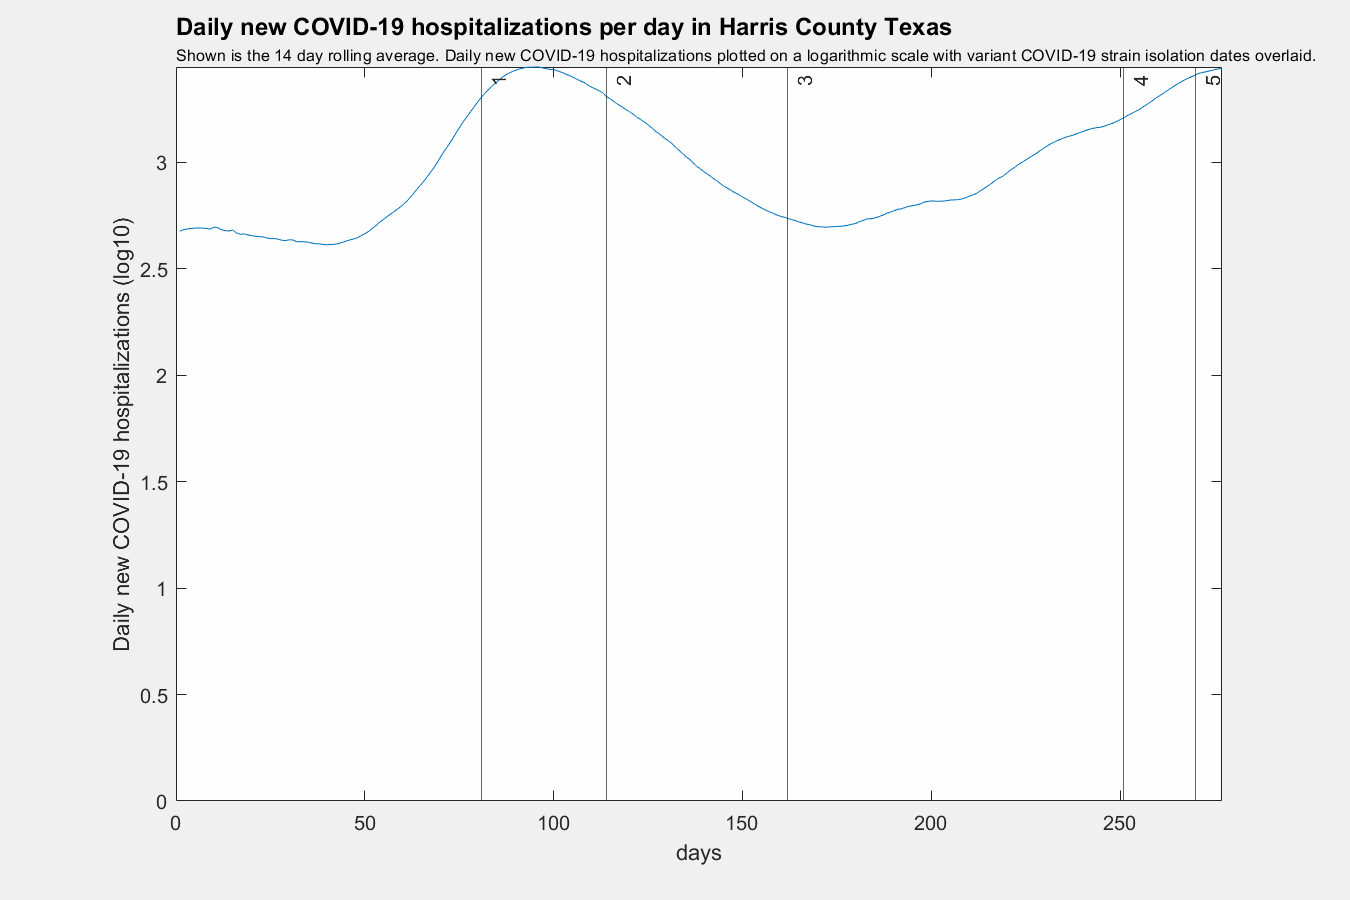
\includegraphics[width=\linewidth]{images/harris_hospitalizations_strains_log.png}
	\caption{Harris County is in the middle of it's first local maximum in daily new COVID-19 cases per day when the California COVID-19 variant, CAL.20C (indicated in the figure as line 1), is first isolated. Shortly after the UK COVID-19 variant, B.1.1.7 (indicated in the figure as line 3), is isolated, daily new COVID-19 hospitalizations in Harris County begins to rise.  }
	\label{fig:images/harris_hospitalizations_strains_logLabel}
\end{figure}

\FloatBarrier

\indent In figures 12-20, the 14 day moving average of daily new COVID-19 hospitalizations per day in 9 counties is displayed on a logarithmic scale ($log_{10}$) with vertical line overlays representing the dates in which five sophisticated COVID-19 variant strains were first detected in their respective population. The counties assessed are Miami-Dade County, Florida; Broward County, Florida; Orange County, Florida; Los Angeles County, California; San Bernardino County, California; San Francisco County, California; Travis County, Texas; Dallas County, Texas; and Harris County, Texas. The genomic isolation dates of the COVID-19 variant strains in figures 12-20 are belonging to: CAL.20C (of lineage B.1.429), first isolated in California; B.1.1.207, first isolated in Nigeria; B.1.1.7 (aka VOC-202012/01, and as lineage B.1.1.7, or 20I/501Y.V1), first isolated in the United Kingdom; B.1.351 (aka 20H/501Y.V2, formerly known as 20C/501Y.V2), first isolated in South Africa; and P.1 (of lineage B.1.1.248), first isolated in Tokyo, and colloquially referred to as the Brazilian variant. 

\indent By the time in which the first COVID-19 variant strain, CAL.20C (indicated in the figure as line 1), is genetically isolated in California, 100\% of the respective counties are increasing in daily new COVID-19 hospitalizations per day. Additionally, the CAL.20C variant strain arrives after 100\% of the counties have already experienced their first rise and fall in daily new COVID-19 hospitalizations. 

\indent The variant strain originating from Nigeria, B.1.1.207 (indicated in the figure as line 2), arrives in 100\% of the counties as they are on the downhill trek of their second wave in daily new COVID-19 hospitalizations per day. 

\indent In 66.7\% of the counties, the isolation date of the UK COVID-19 variant, B.1.1.7 (indicated in the figure as line 3), arrives at the base of a third wave in daily new COVID-19 hospitalizations per day. In 22.3\% of the counties, B.1.1.7 arrives as they are still maintaining a downhill trend in daily new COVID-19 hospitalizations per day. Additionally, in 11.1\% of the counties, the isolation of B.1.1.7 arrives amidst a rapidly fluctuating oscillation in daily new COVID-hospitalizations per day. 

\indent The isolation dates of the COVID-19 variant strains from South Africa and Brazil, also known as B.1.351 and P.1 (indicated in the figure as line 4 and line 5), occur with one month relative to each other. At the time of their respective genetic isolation, 66.7\% of the counties are trending upwards in daily new COVID-19 hospitalizations per day. Conversely 33.3\% of the counties are decreasing in daily new COVID-19 hospitalizations as the South African variant and Brazilian variant are isolated. 


\indent 

 
\FloatBarrier
\vspace{5mm}
\section*{COVID-19 variants and daily new fatalities}


\begin{figure}[!h]
	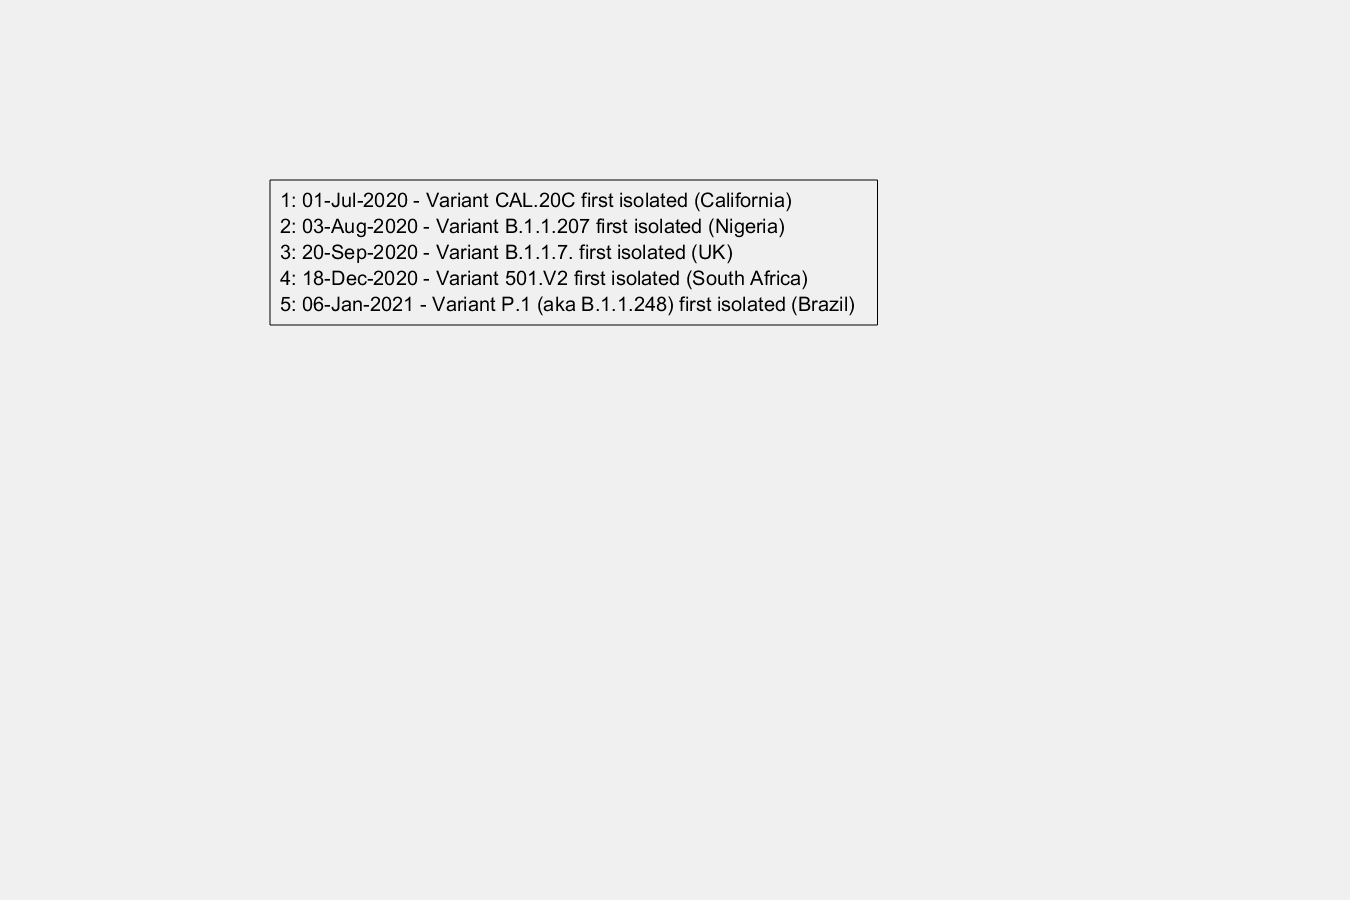
\includegraphics[width=\linewidth]{legends/variant_strains_legend.png}
	\caption{Listed above are five uniquely infectious variant strains of COVID-19,  listed corresponding to the date in which they were first genetically sequenced and isolated in their respective region.}
	\label{fig:legends/variant_strains_legendLabel}
\end{figure}

\begin{figure}[!h]
	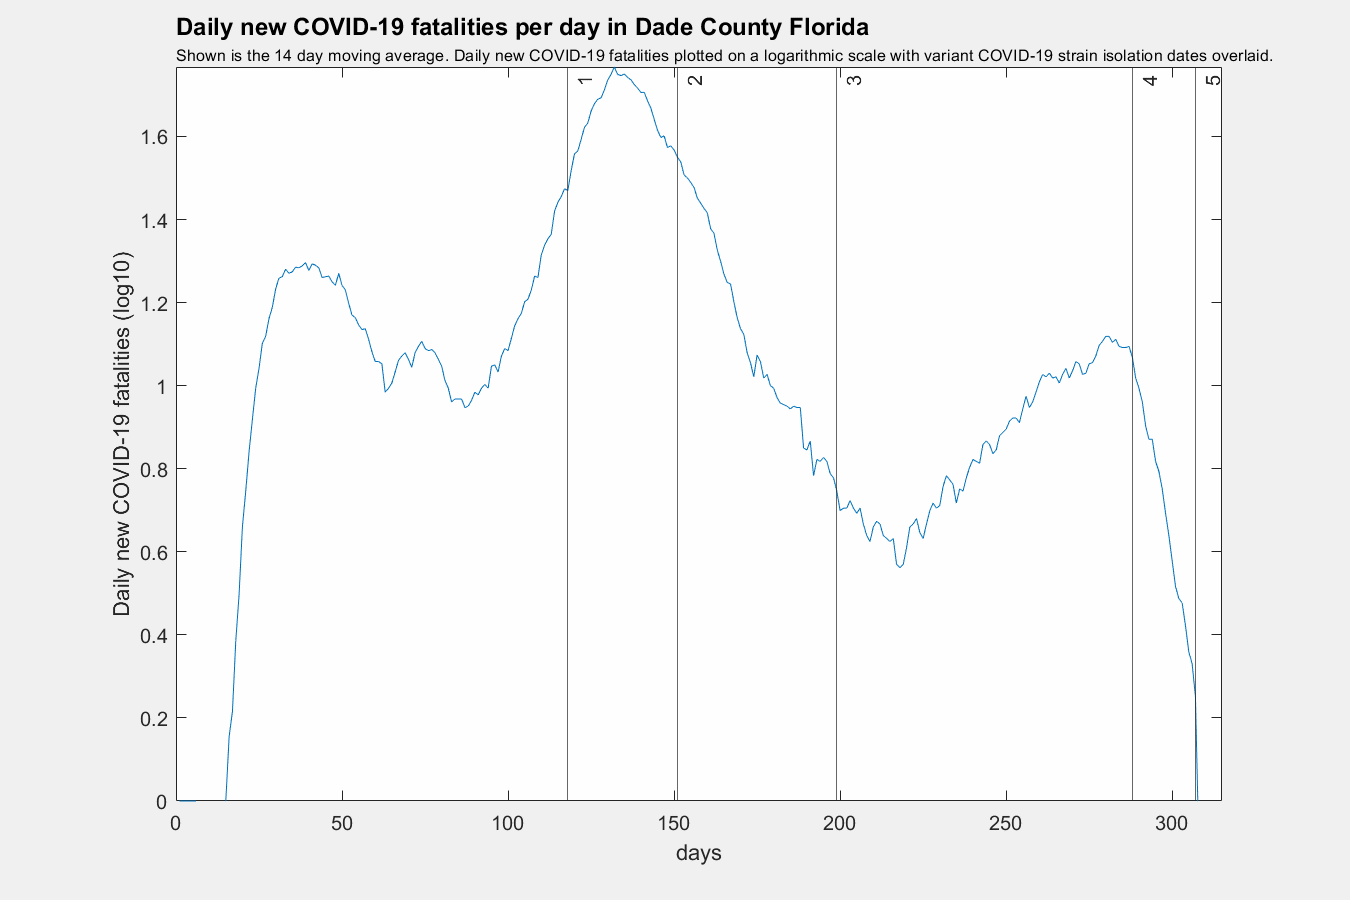
\includegraphics[width=\linewidth]{images/dade_fatalities_strains_log.png}
	\caption{Daily new COVID-19 fatalities in Miami-Dade County were at a global maximum during the isolation date of the COVID-19 variant strain CAL.20C (indicated in the figure as line 1), and B.1.1.207 (indicated in the figure as line 2). The deaths in Miami-Dade County rose again approximately 20 days after the UK COVID-19 variant, B.1.1.7 (indicated in the figure as line 3), was isolated in the United Kingdom.   }
	\label{fig:images/dade_fatalities_strains_logLabel}
\end{figure}

\begin{figure}[!h]
	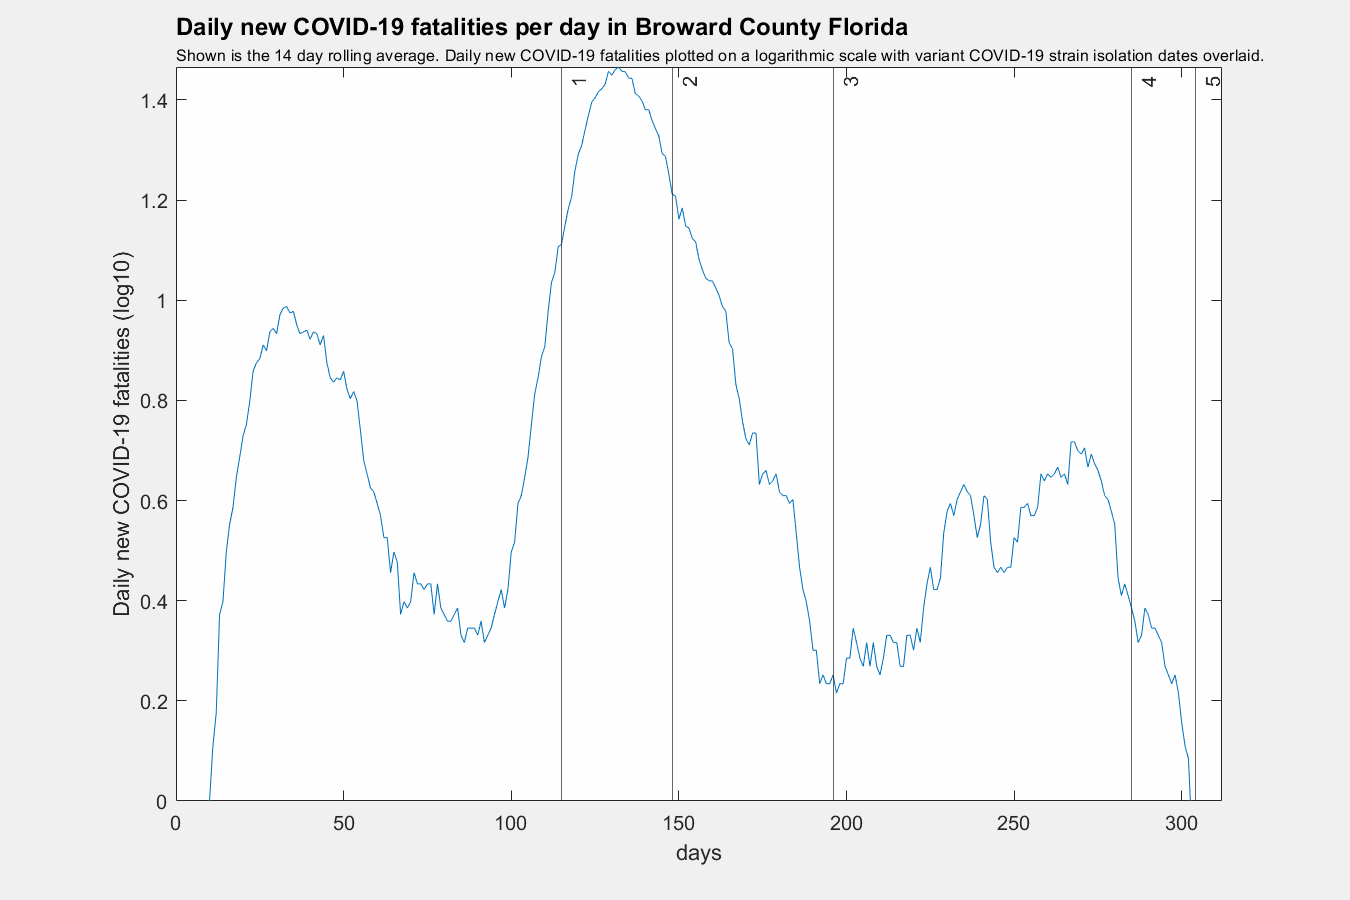
\includegraphics[width=\linewidth]{images/broward_fatalities_strains_log.png}
	\caption{Broward County is headed towards the peak of it's second wave in daily new COVID-19 fatalities as the variant from California, CAL.20C (indicated in the figure as line 1), is first isolated.Daily new COVID-19 fatalities in Broward County rises for a third time just at the COVID-19 variant from the UK, B.1.1.7 (indicated in the figure as line 3), is isolated.}
	\label{fig:images/broward_fatalities_strains_logLabel}
\end{figure}


\begin{figure}[!h]
	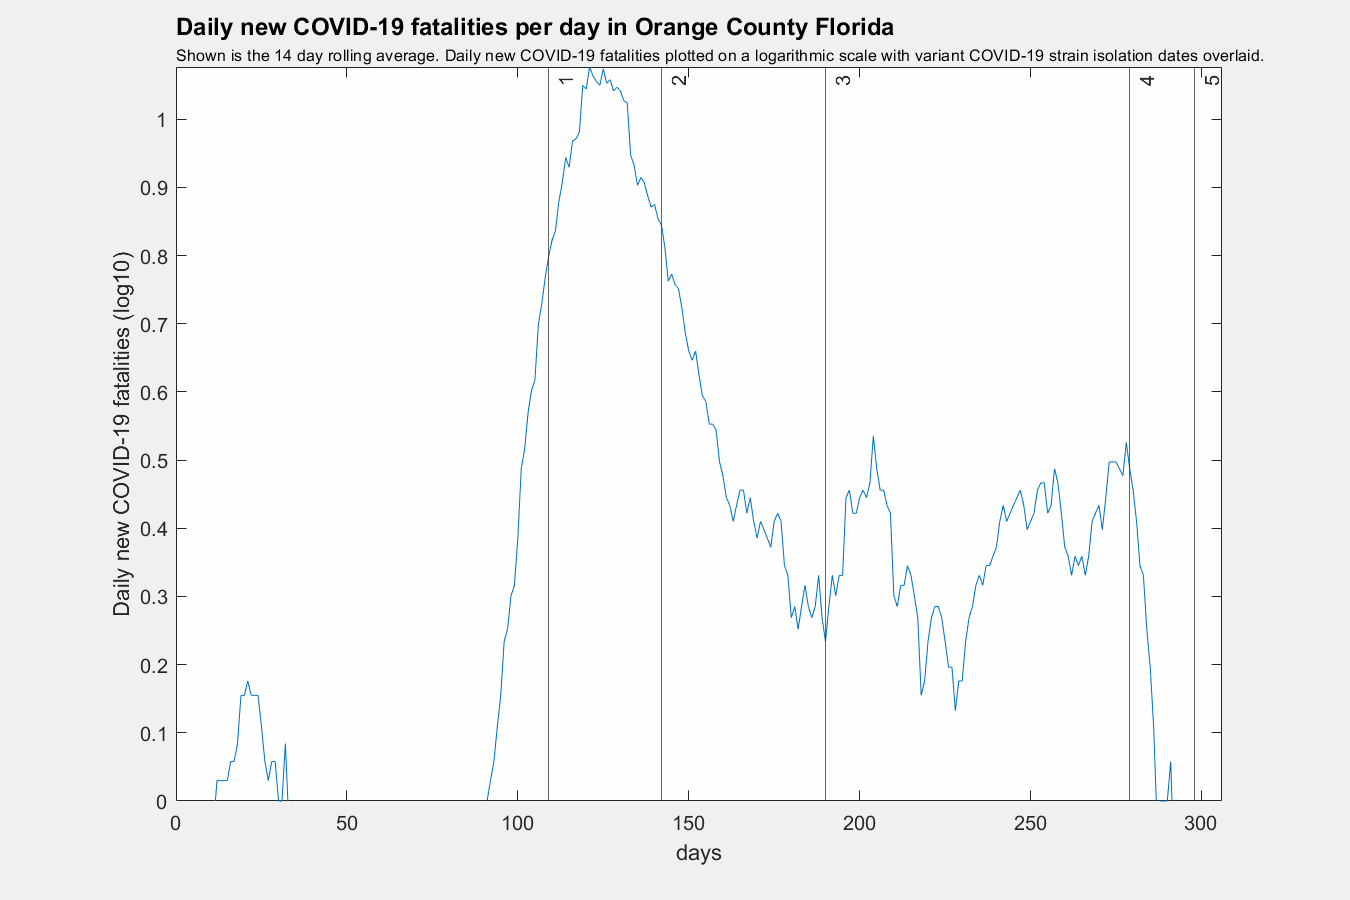
\includegraphics[width=\linewidth]{images/orange_fatalities_strains_log.png}
	\caption{When the COVID-19 variant from California, CAL.20C (indicated in the figure as line 1), is first detected, Orange County is approaching it's highest rate in daily new COVID-19 fatalities per day since the initiation of daily COVID-19 data reporting.  }
	\label{fig:images/orange_fatalities_strains_logLabel}
\end{figure}


\begin{figure}[!h]
	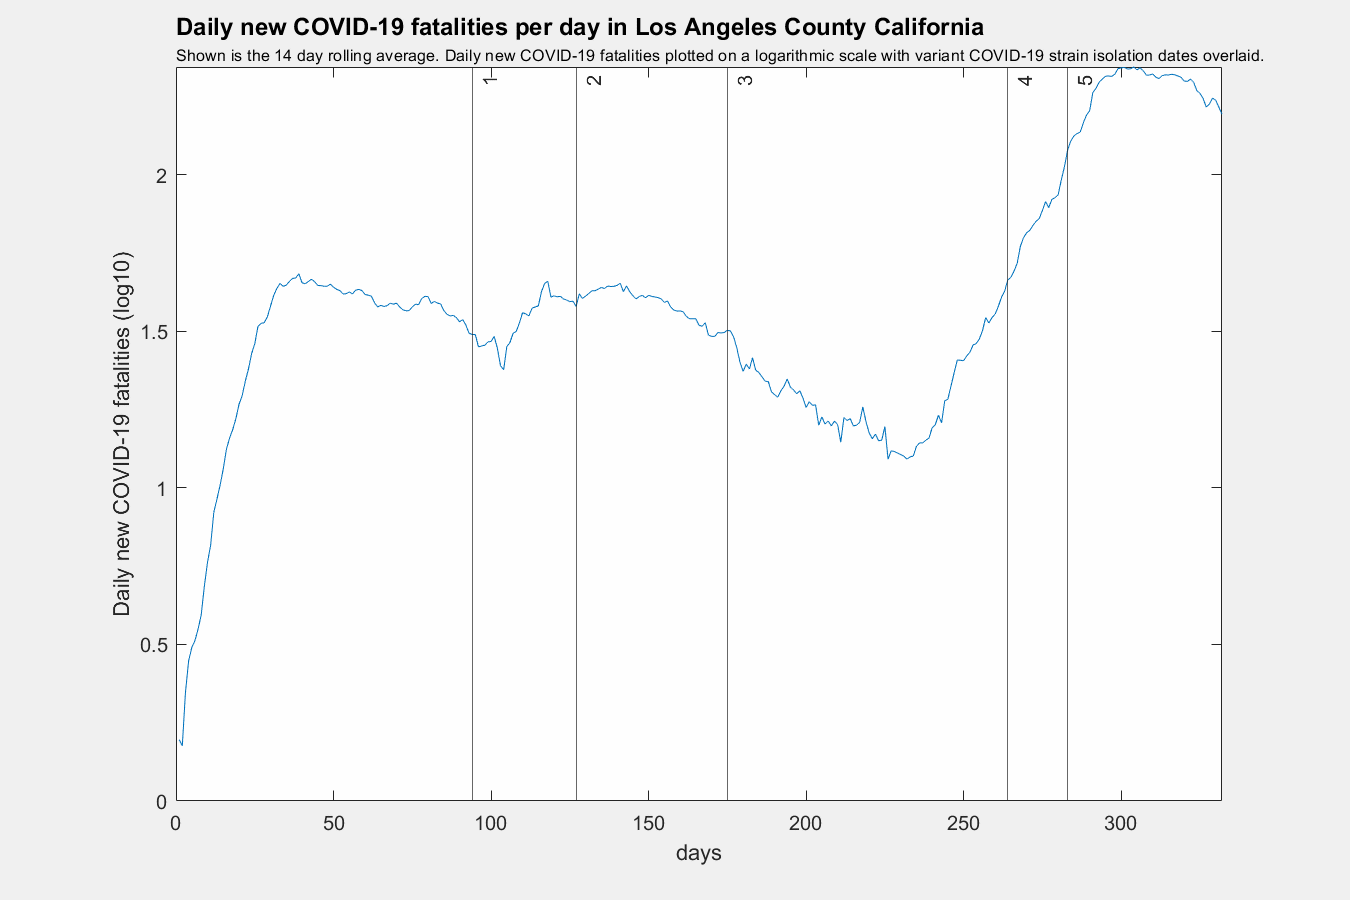
\includegraphics[width=\linewidth]{images/los_angeles_fatalities_strains_log.png}
	\caption{Daily new COVID-19 fatalities per day in Los Angeles County exhibit little fluctuation in their change of rate prior to the isolation of the COVID-19 variant from the UK, B.1.1.7 (indicated in the figure as line 3). However, roughly a month and a half after the isolation of B.1.1.7, daily new COVID-19 fatalities in Los Angeles County begin to steadily climb without any downwards deviation.  }
	\label{fig:images/los_angeles_fatalities_strains_logLabel}
\end{figure}

\begin{figure}[!h]
	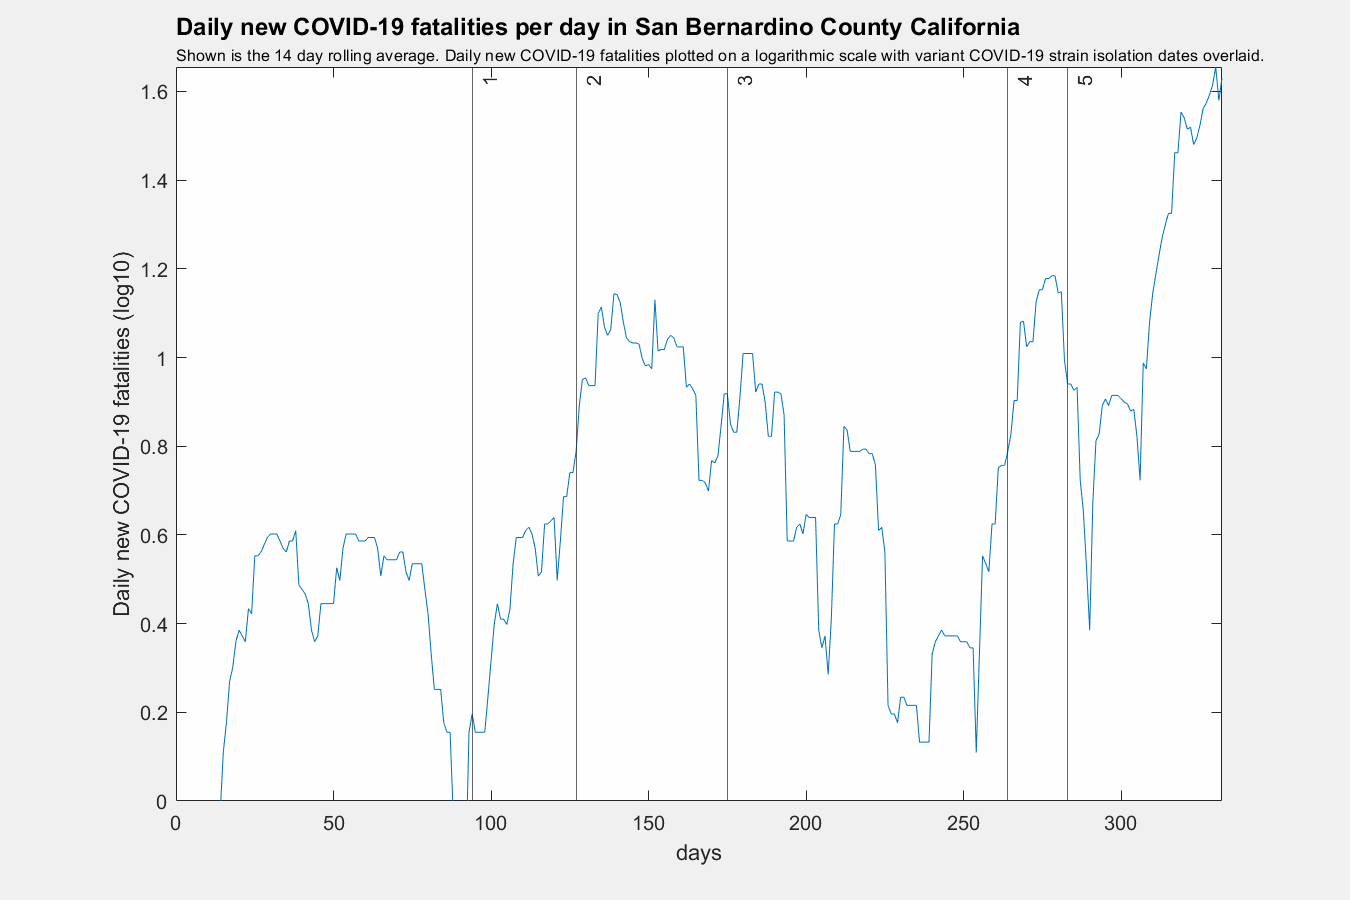
\includegraphics[width=\linewidth]{images/san_bernardino_fatalities_strains_log.png}
	\caption{San Bernardino County has thus far exhibited three significant waves in daily new COVID-19 fatalities per day. The first three COVID-19 variant isolation date overlays (belonging to CAL.20C, B.1.1.207, and B.1.1.7) coincide with the rise and fall of the second wave in daily new COVID-19 fatalities per day.The isolation dates of the variants from South Africa and Brazil, also known as B.1.351 and P.1 (indicated in the figure as line 4 and 5), arrive as the third wave in daily new COVID-19 fatalities per day occurs in San Bernardino County.}
	\label{fig:images/san_bernardino_fatalities_strains_logLabel}
\end{figure}


\begin{figure}[!h]
	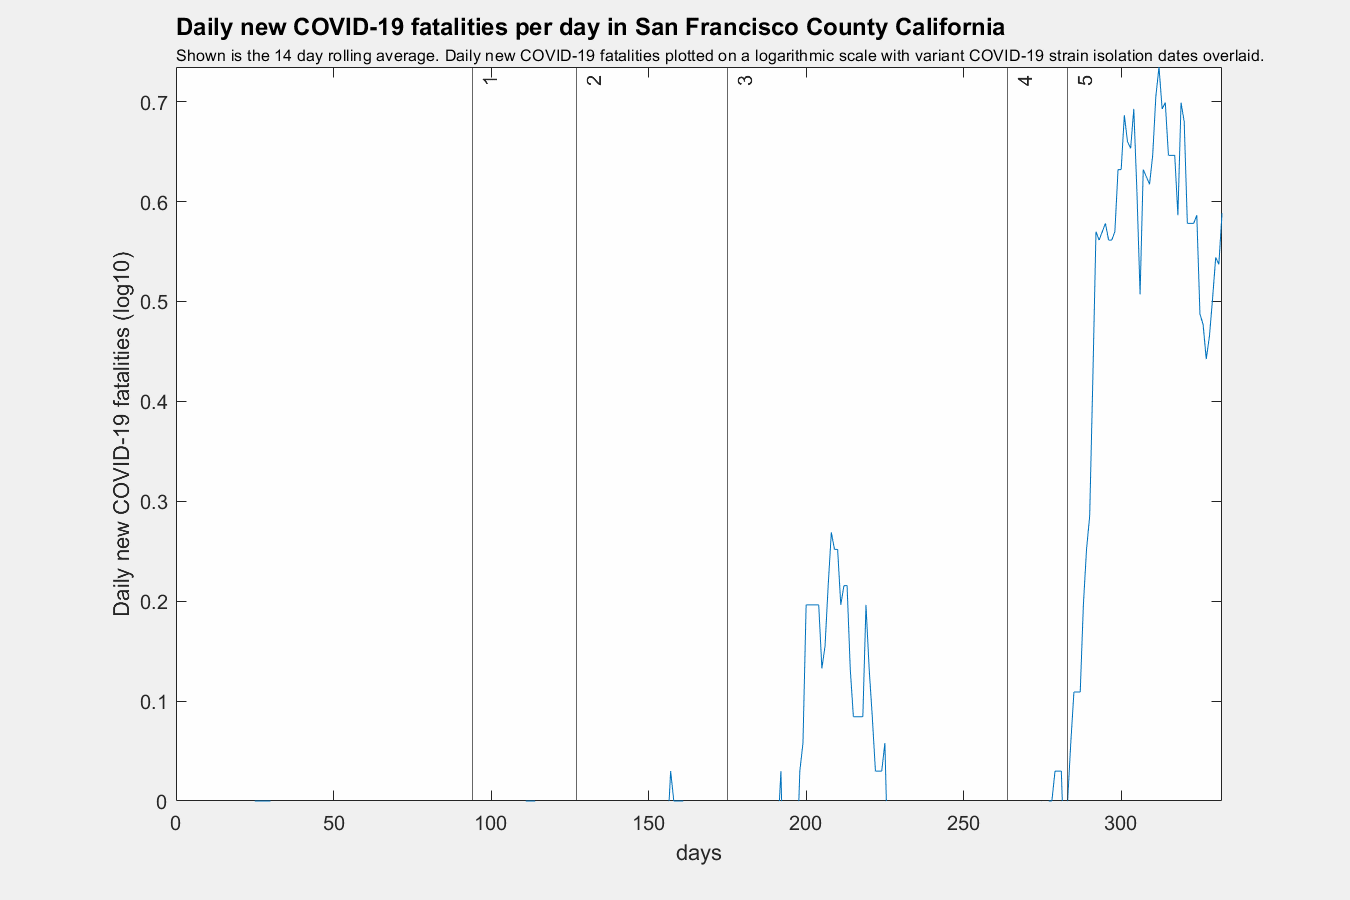
\includegraphics[width=\linewidth]{images/san_francisco_fatalities_strains_log.png}
	\caption{Values reported for daily new COVID-19 fatalities in San Francisco County have been relatively low throughout the first several months of COVID-19 data reporting. Shortly after the isolation of the variant strain from the UK (indicated in the figure as line 3), San Bernardino exhibits a local maximum in daily new COVID-19 fatalities. Additionally, as the variants from South Africa and Brazil are isolated (also known as B.1.351 and P.1, indicated in the figure as line 4 and 5), San Francisco County experiences another, more significant, rise in daily new COVID-19 fatalities per day.}
	\label{fig:images/san_francisco_fatalities_strains_logLabel}
\end{figure}


\begin{figure}[!h]
	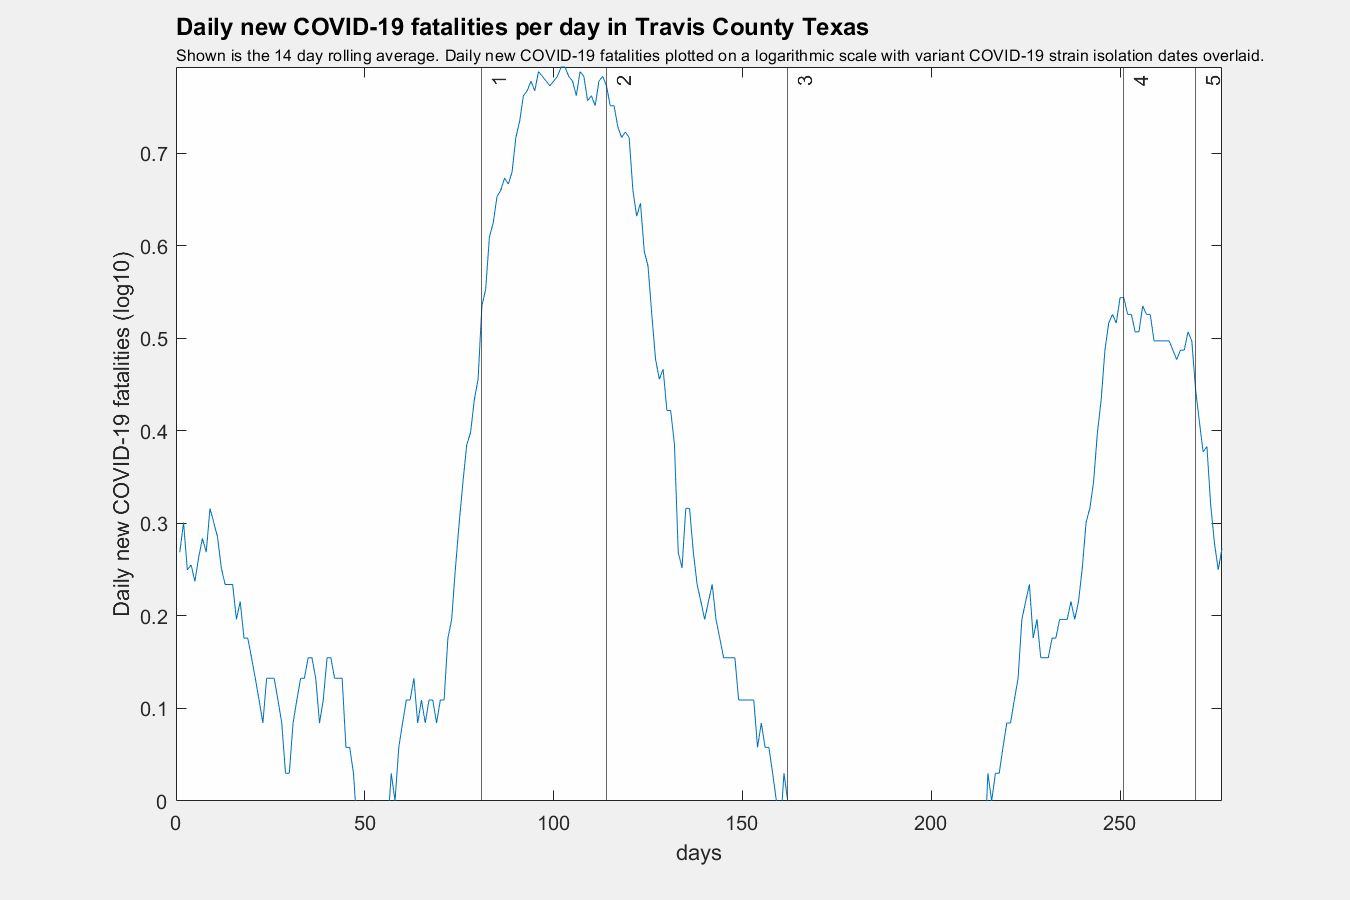
\includegraphics[width=\linewidth]{images/travis_fatalities_strains_log.png}
	\caption{At the time in which the variant from California is isolated (indicated in the figure as line 1), Travis County is approaching a global maximum in daily new COVID-19 fatalities per day. Approximately six weeks after the isolation of the variant from the UK (indicated in the figure as line 3), Travis County experiences a local maximum in daily new COVID-19 fatalities per day. }
	\label{fig:images/travis_fatalities_strains_logLabel}
\end{figure}

\begin{figure}[!h]
	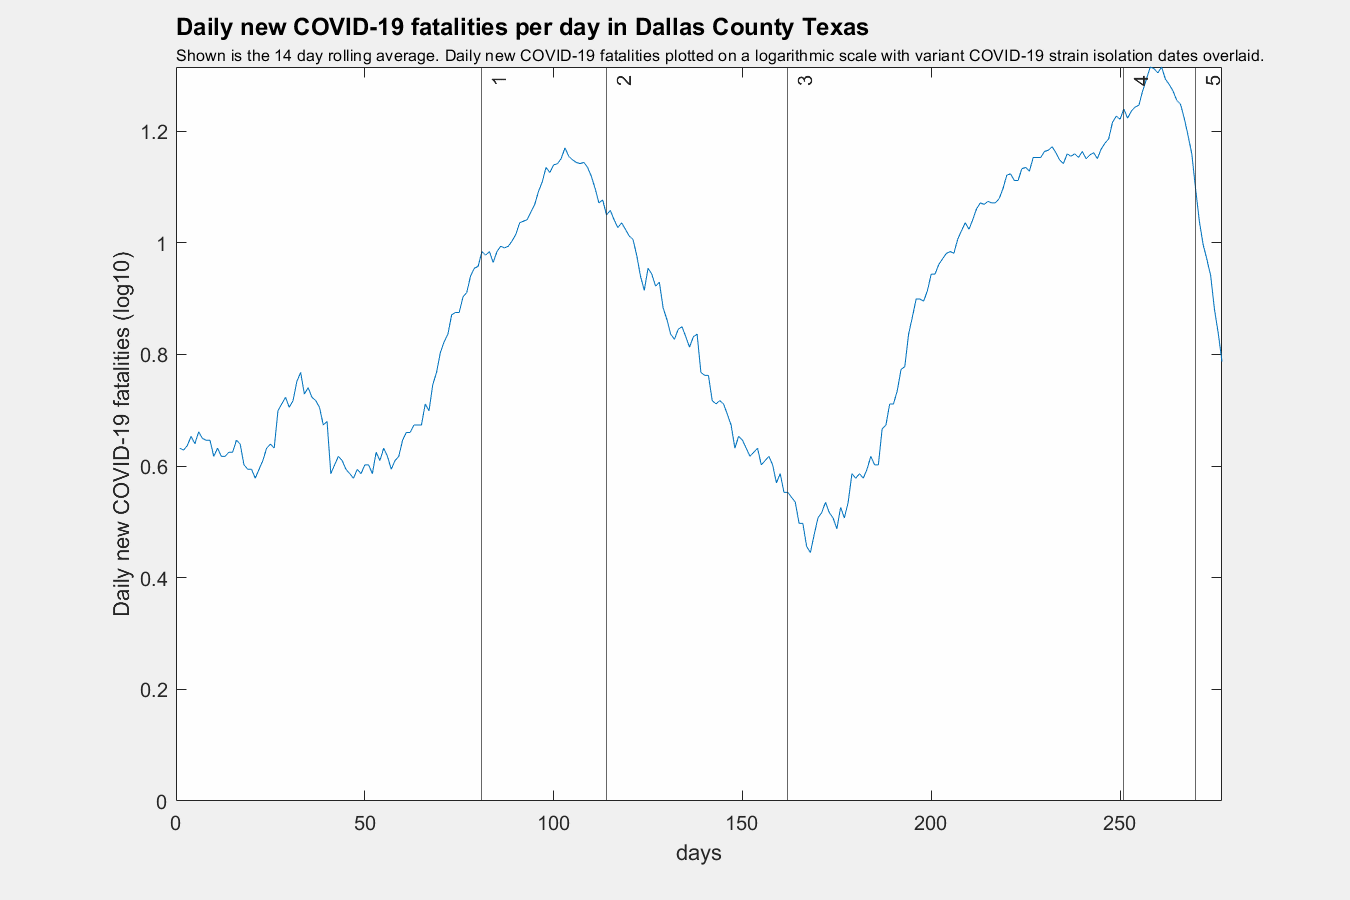
\includegraphics[width=\linewidth]{images/dallas_fatalities_strains_log.png}
	\caption{When the COVID-19 variant from California, CAL.20C (indicated in the figure as line 1), is first isolated, daily new COVID-19 fatalities per day are headed uphill in Dallas County. Conversely, when the variant from the UK, B.1.1.7 (indicated in the figure as line 3) is isolated, daily new COVID-19 fatalities per day are at a local minimum. The isolation of B.1.351 and P.1 (associated with South Africa and Brazil, indicated in the figure as line 4 and 5), coincide with a local maximum in daily new COVID-19 fatalities per day.}
	\label{fig:images/dallas_fatalities_strains_logLabel}
\end{figure}

\begin{figure}[!h]
	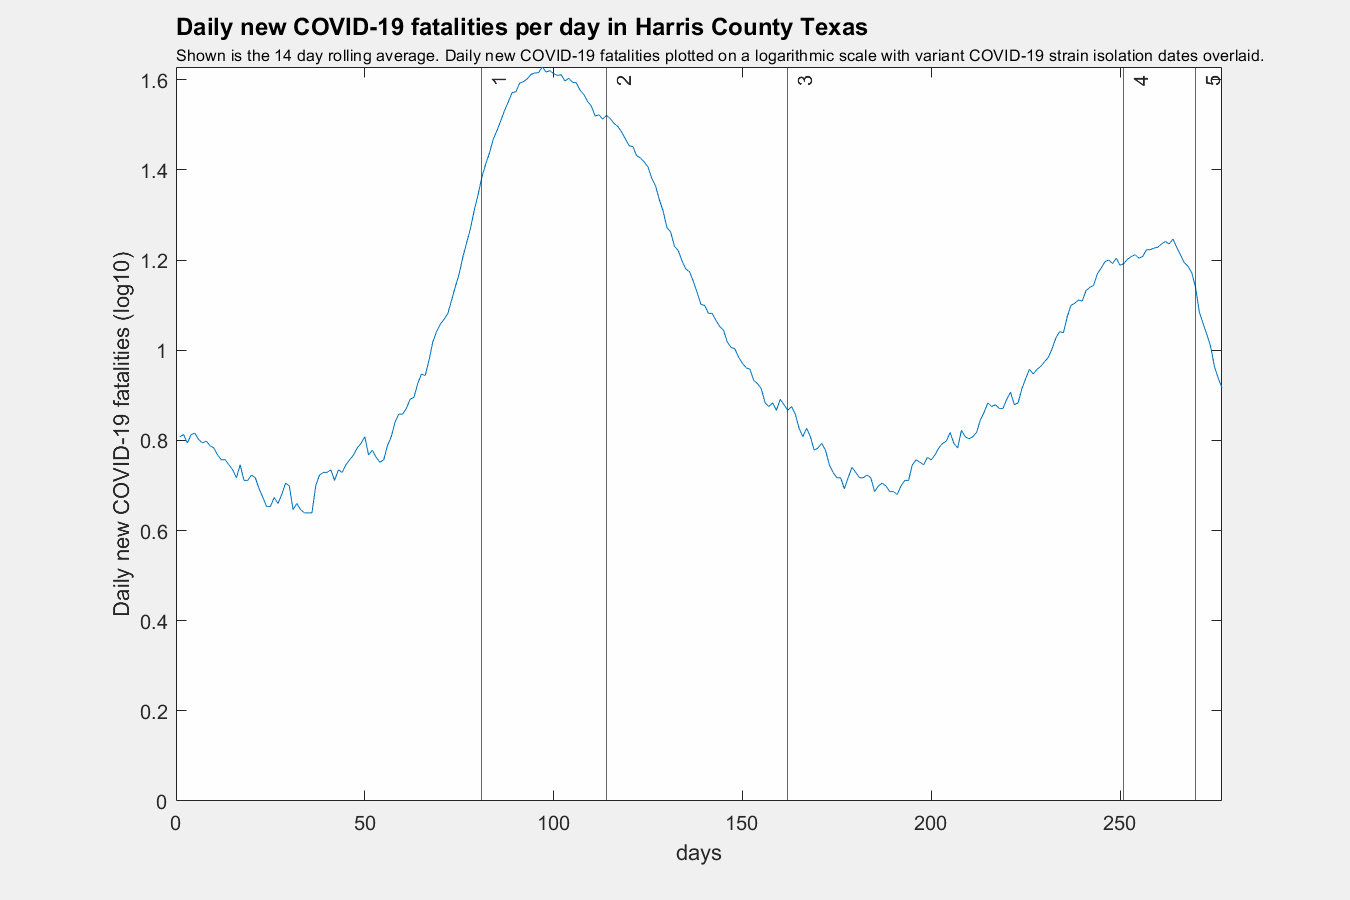
\includegraphics[width=\linewidth]{images/harris_fatalities_strains_log.png}
	\caption{The isolation dates of COVID-19 variants from California and Nigeria (also referred to as CAL.20C and B.1.1.207, indicated in the figure as line 1 and 2) coincide with a global maximum in daily new COVID-19 fatalities in Harris County. Conversely, the isolation date of the variant strain from the UK (also referred to as B.1.1.7, indicated in the figure as line 3) is overlaid a local minimum in daily new COVID-19 fatalities per day. Meanwhile, B.1.351 (South Africa, line 4) and P.1 (Brazil, line 5) are overlaid a local maximum in daily new fatalities per day. }
	\label{fig:images/harris_fatalities_strains_logLabel}
\end{figure}

\FloatBarrier

\indent In figures 22-30, the 14 day moving average of daily new COVID-19 fatalities per day in 9 counties is displayed on a logarithmic scale ($log_{10}$) with vertical line overlays representing the dates in which five sophisticated COVID-19 variant strains were first detected in their respective population. The counties assessed are Miami-Dade County, Florida; Broward County, Florida; Orange County, Florida; Los Angeles County, California; San Bernardino County, California; San Francisco County, California; Travis County, Texas; Dallas County, Texas; and Harris County, Texas. The genomic isolation dates of the COVID-19 variant strains in figures 22-30 are belonging to: CAL.20C (of lineage B.1.429), first isolated in California; B.1.1.207, first isolated in Nigeria; B.1.1.7 (aka VOC-202012/01, and as lineage B.1.1.7, or 20I/501Y.V1), first isolated in the United Kingdom; B.1.351 (aka 20H/501Y.V2, formerly known as 20C/501Y.V2), first isolated in South Africa; and P.1 (of lineage B.1.1.248), first isolated in Tokyo, and colloquially referred to as the Brazilian variant.

\indent When CAL.20C is genetically isolated in California, 77.8\% of the counties assessed in the study are on the rising end of a local maximum in daily new COVID-19 fatalities per day. Additionally, in 77.8\% of the counties, the isolation date of CAL.20C coincides with the most deadly time of the pandemic for the respective counties. At this date, the counties at hand are undergoing the highest rate in daily new COVID-19 fatalities per day since daily COVID-19 reporting was initiated. In 11.1\% of the counties, daily new COVID-19 fatalities are at the brink of a new, local maximum when CAL.20C is isolated. Further, in 11.2\% of the counties, CAL.20C coincides with extremely low reportings for daily new COVID-19 fatalities in which the isolation date is overlaid a non-existent plot, as reportings are so low. 

\indent As the variant strain from Nigeria, also known as B.1.1.207, is first isolated, 66.7\% of the counties are on the downhill trek of a local maximum in daily new COVID-19 fatalities per day. Conversely, in 22.2\% of the counties, the isolation date of B.1.1.207 coincides with the peak of a local maximum in daily new COVID-19 fataities per day. Additionally, in 11.2\% of the counties, reporting of daily new COVID-19 fatalities are so low that the isolation date of B.1.1.207 is overlaid a non-existent plot. 

\indent When the variant strain from the United Kingdom, also referred to as B.1.1.7, is isolated, 77.8\% of the counties are displaying a local minimum in daily new COVID-19 fatalities per day. In 11.1\% of the counties, namely San Francisco County, reportings for daily new COVID-19 cases per day are so low that the isolation date overlay for B.1.1.7 occurs prior to the availability of significant data. Further, in 11.2\% of the counties, the isolation of B.1.1.7 occurs during a local maximum in daily new COVID-19 fatalities per day. 

\indent The genetic sequencing of COVID-19 variants B.1.351 and P.1 (associated with South Africa and Tokyo, respectively), occur relatively close in time to one another. At the time in which these two variant strains are isolated, 33.4\% of the counties are displaying a rapid drop towards single integer values in daily new COVID-19 fatalities. In 66.7\% of the counties, the isolation date of B.1.351 and P.1 coincide with a local maximum in daily new COVID-19 fatalities. 

 
\FloatBarrier
\vspace{5mm}

\section*{The post-holiday surge; holidays and the daily COVID-19 case count}

\begin{figure}[!h]
	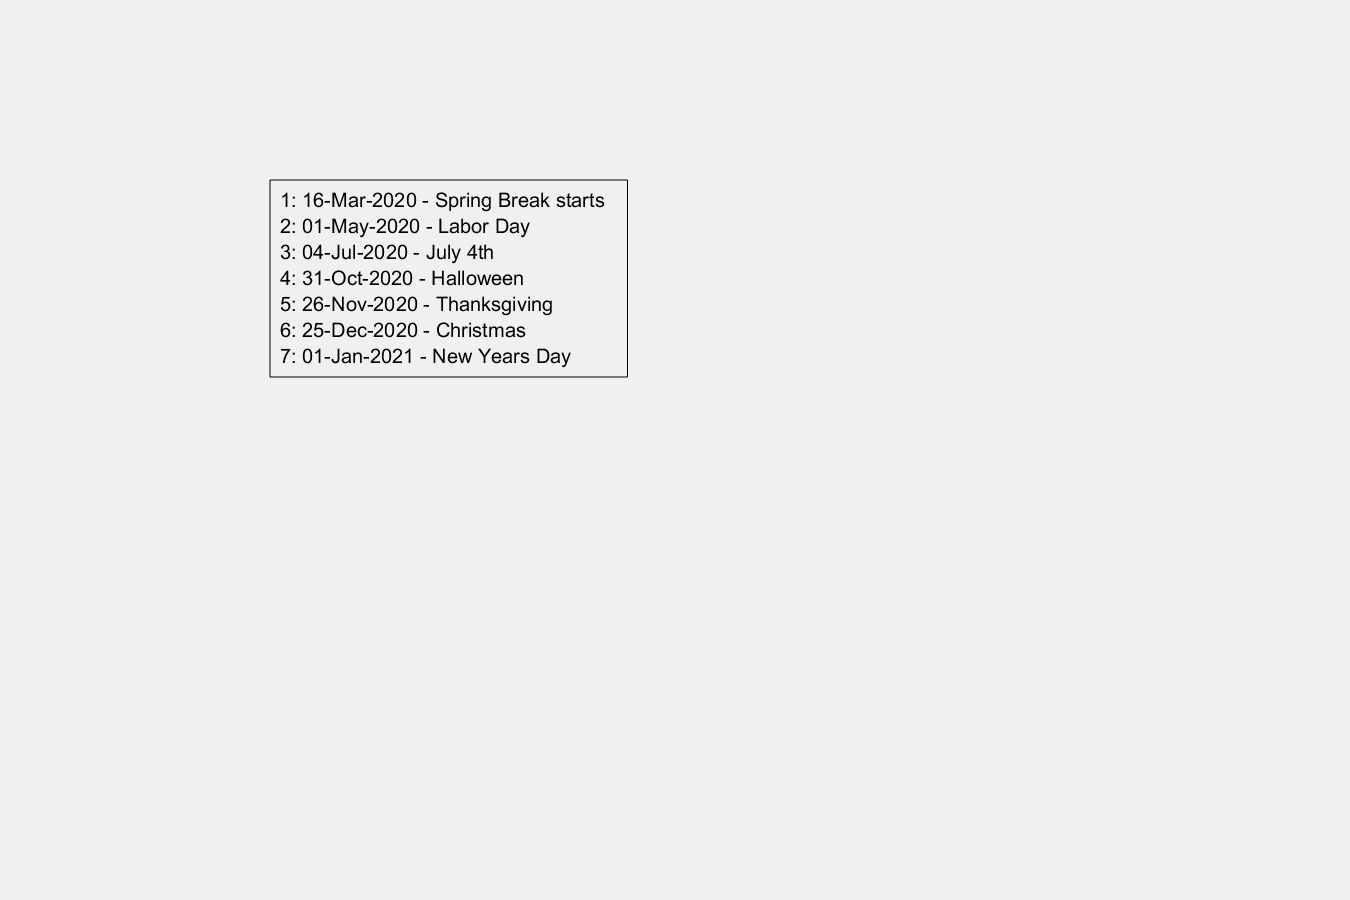
\includegraphics[width=\linewidth]{legends/holiday_legend.png}
	\caption{}
	\label{fig:legends/holiday_legendLabel}
\end{figure}

\begin{figure}[!h]
	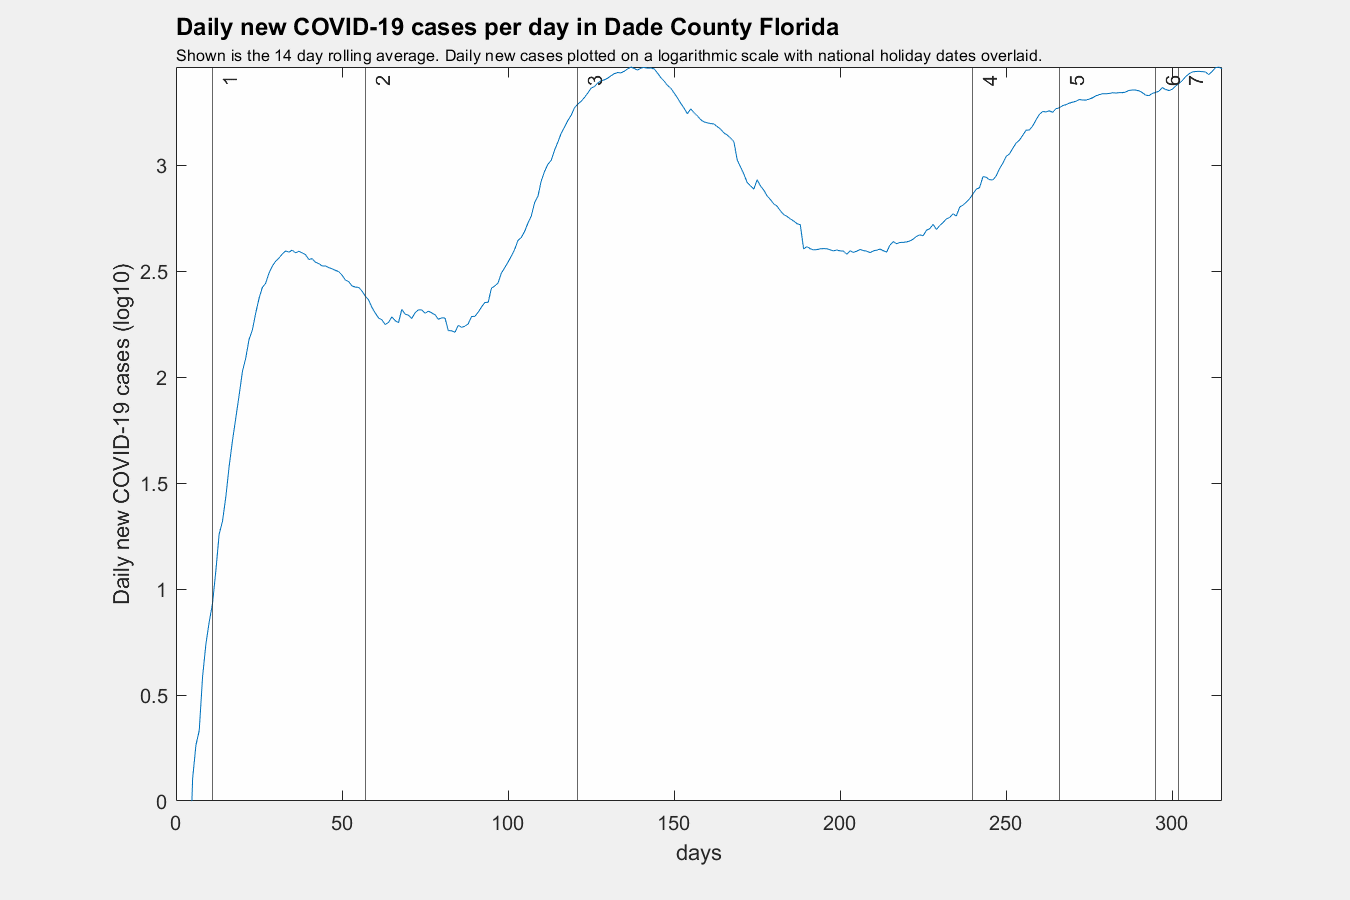
\includegraphics[width=\linewidth]{images/dade_cases_holiday_log.png}
	\caption{}
	\label{fig:images/dade_cases_holiday_logLabel}
\end{figure}

\begin{figure}[!h]
	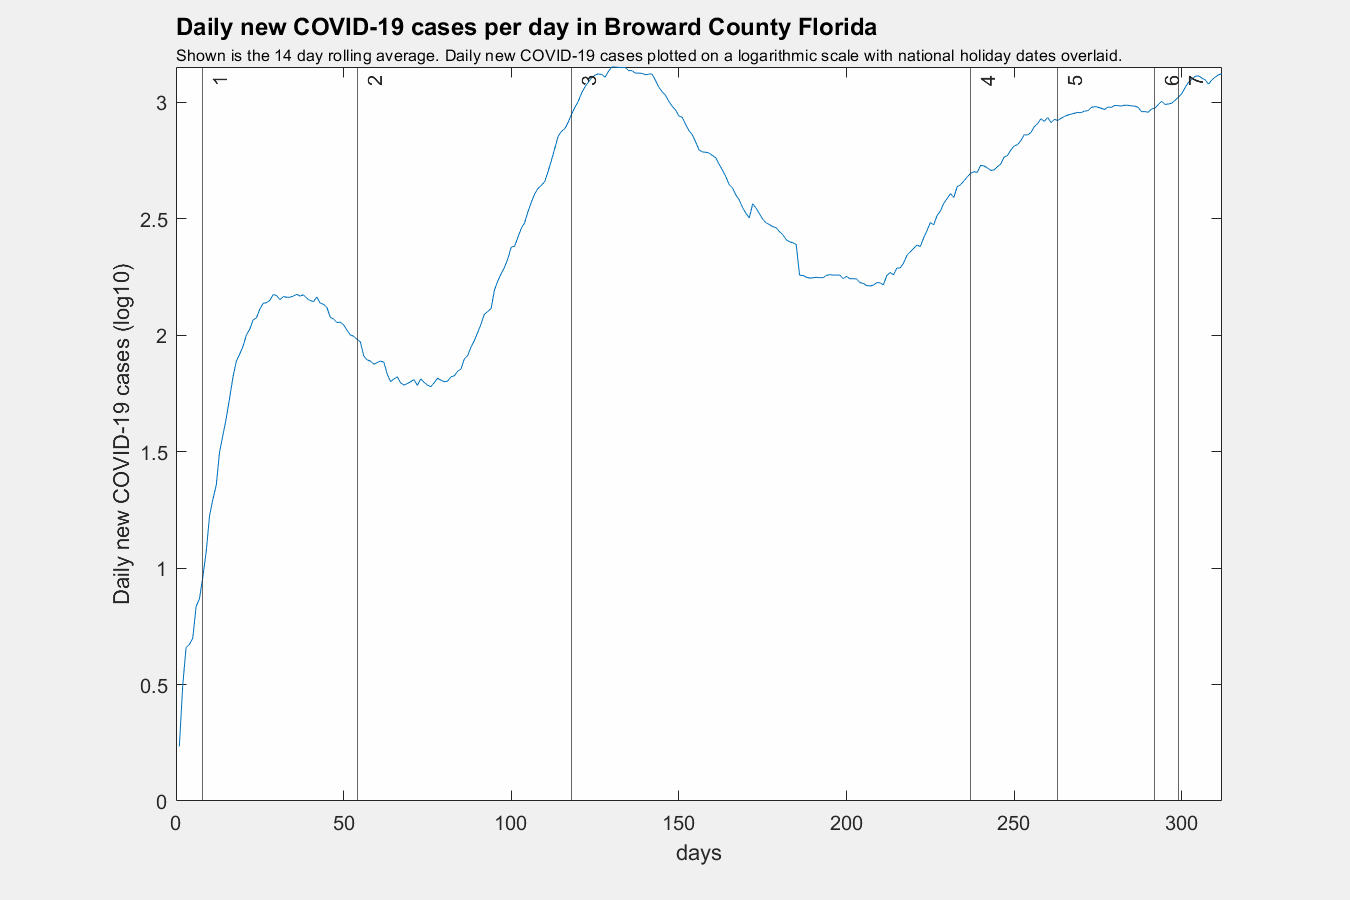
\includegraphics[width=\linewidth]{images/broward_cases_holiday_log.png}
	\caption{}
	\label{fig:images/broward_cases_holiday_logLabel}
\end{figure}

\begin{figure}[!h]
	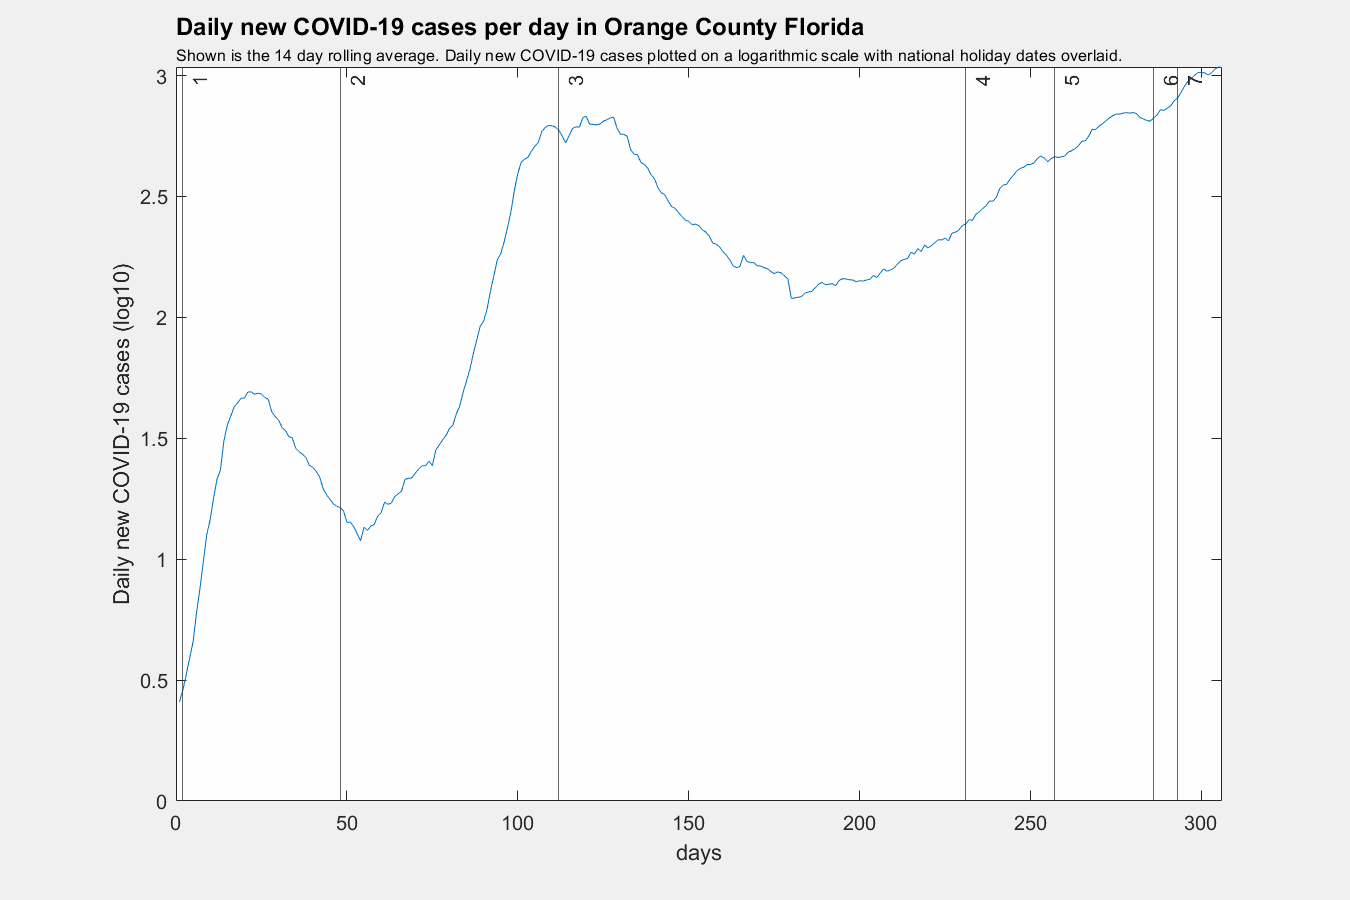
\includegraphics[width=\linewidth]{images/orange_cases_holiday_log.png}
	\caption{}
	\label{fig:images/orange_cases_holiday_logLabel}
\end{figure}

\begin{figure}[!h]
	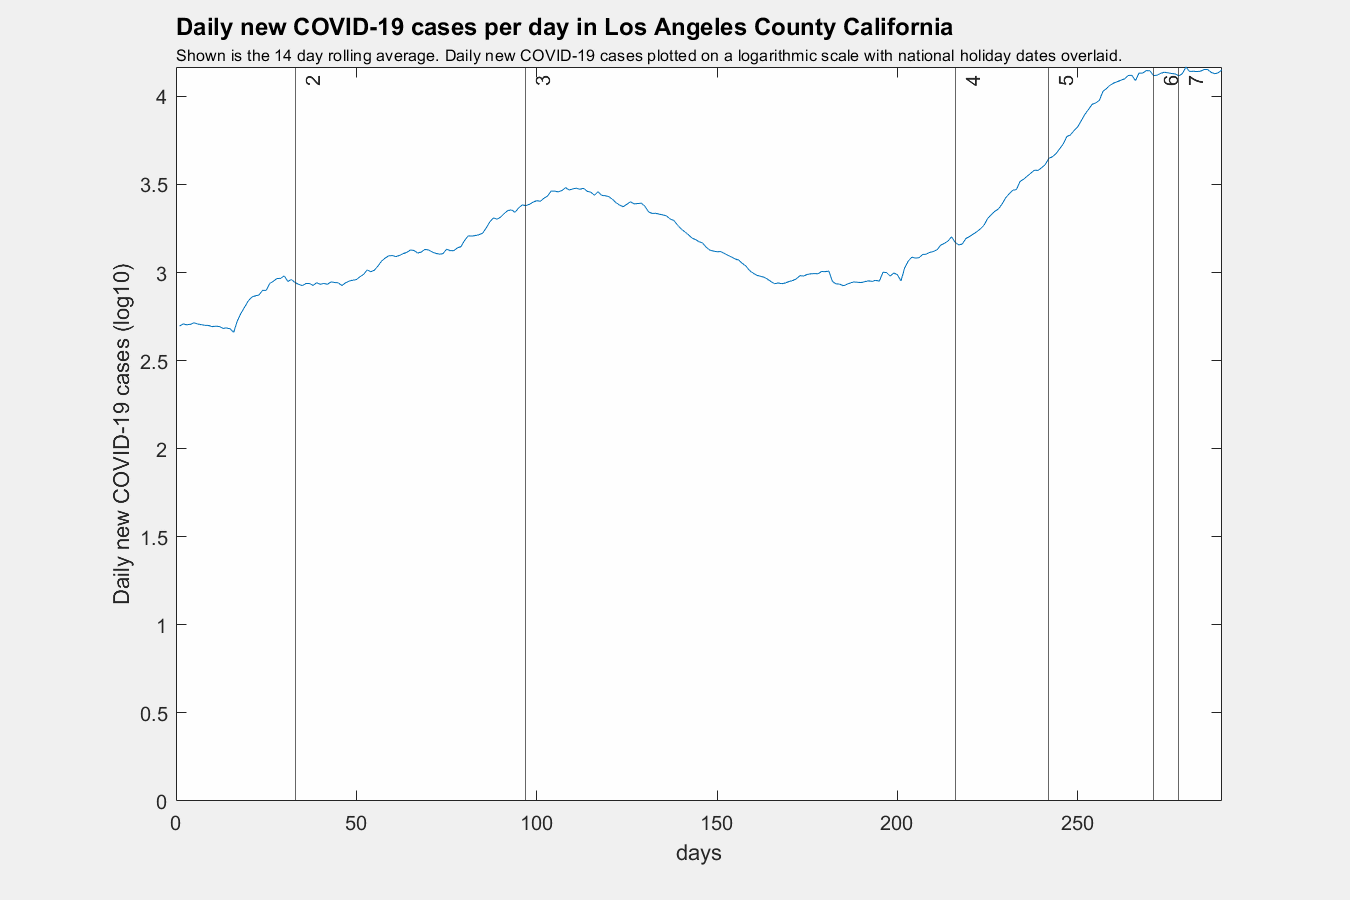
\includegraphics[width=\linewidth]{images/los_angeles_cases_holiday_log.png}
	\caption{}
	\label{fig:images/los_angeles_cases_holiday_logLabel}
\end{figure}


\begin{figure}[!h]
	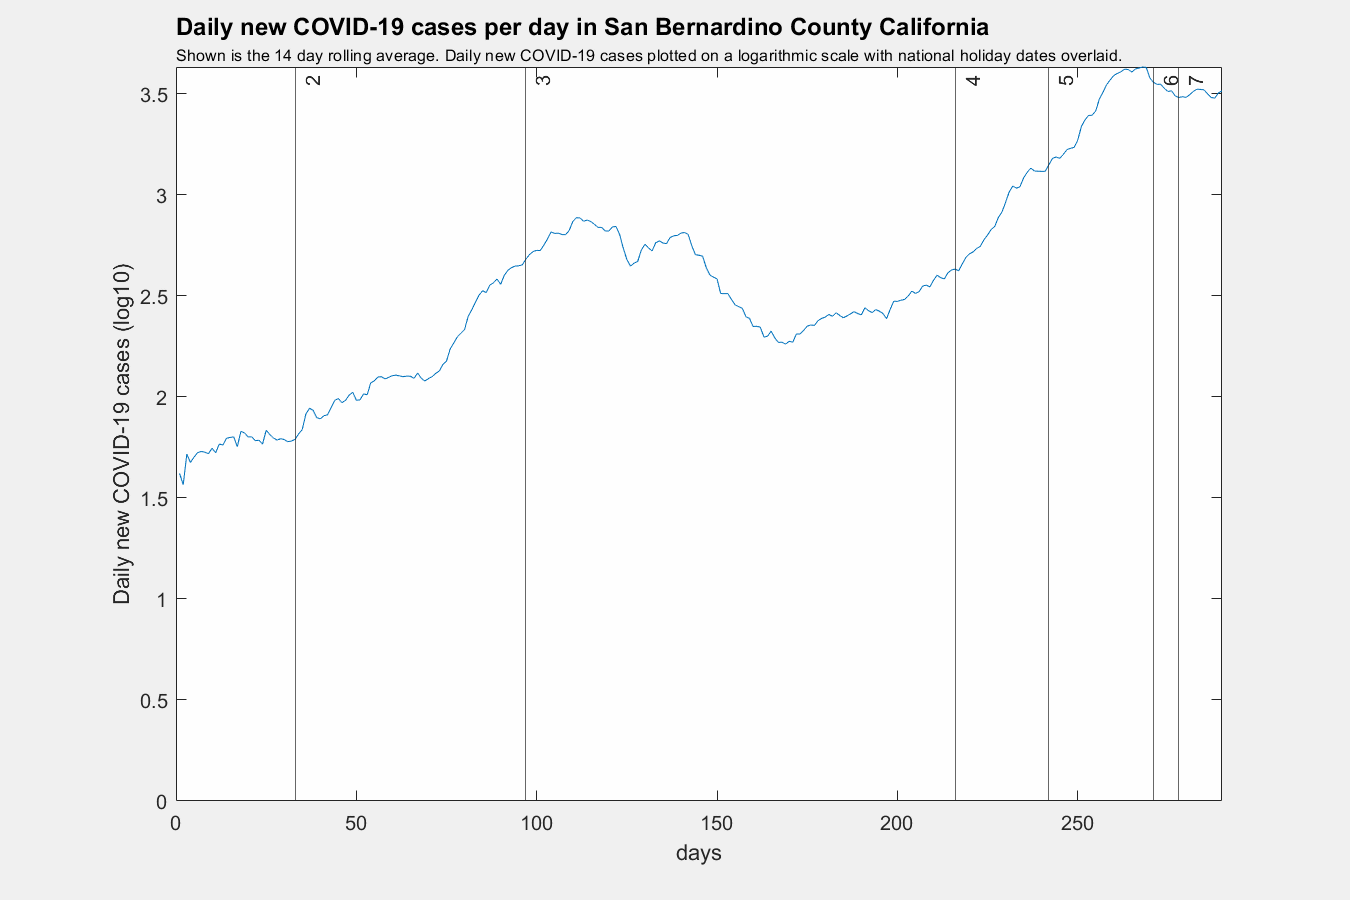
\includegraphics[width=\linewidth]{images/san_bernardino_cases_holiday_log.png}
	\caption{}
	\label{fig:images/san_bernardino_cases_holiday_logLabel}
\end{figure}


\begin{figure}[!h]
	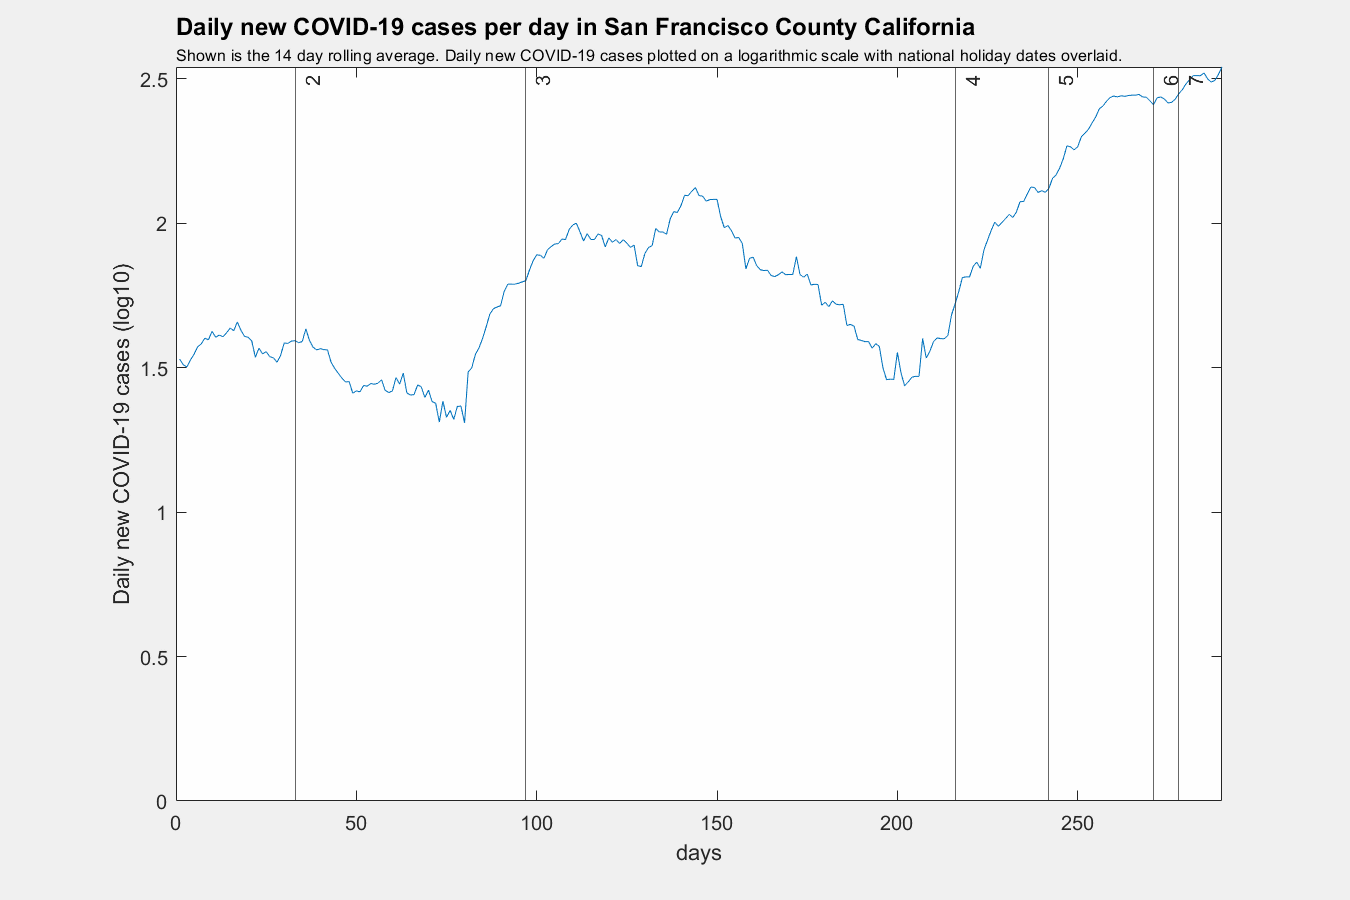
\includegraphics[width=\linewidth]{images/san_francisco_cases_holiday_log.png}
	\caption{}
	\label{fig:images/san_francisco_cases_holiday_logLabel}
\end{figure}


\begin{figure}[!h]
	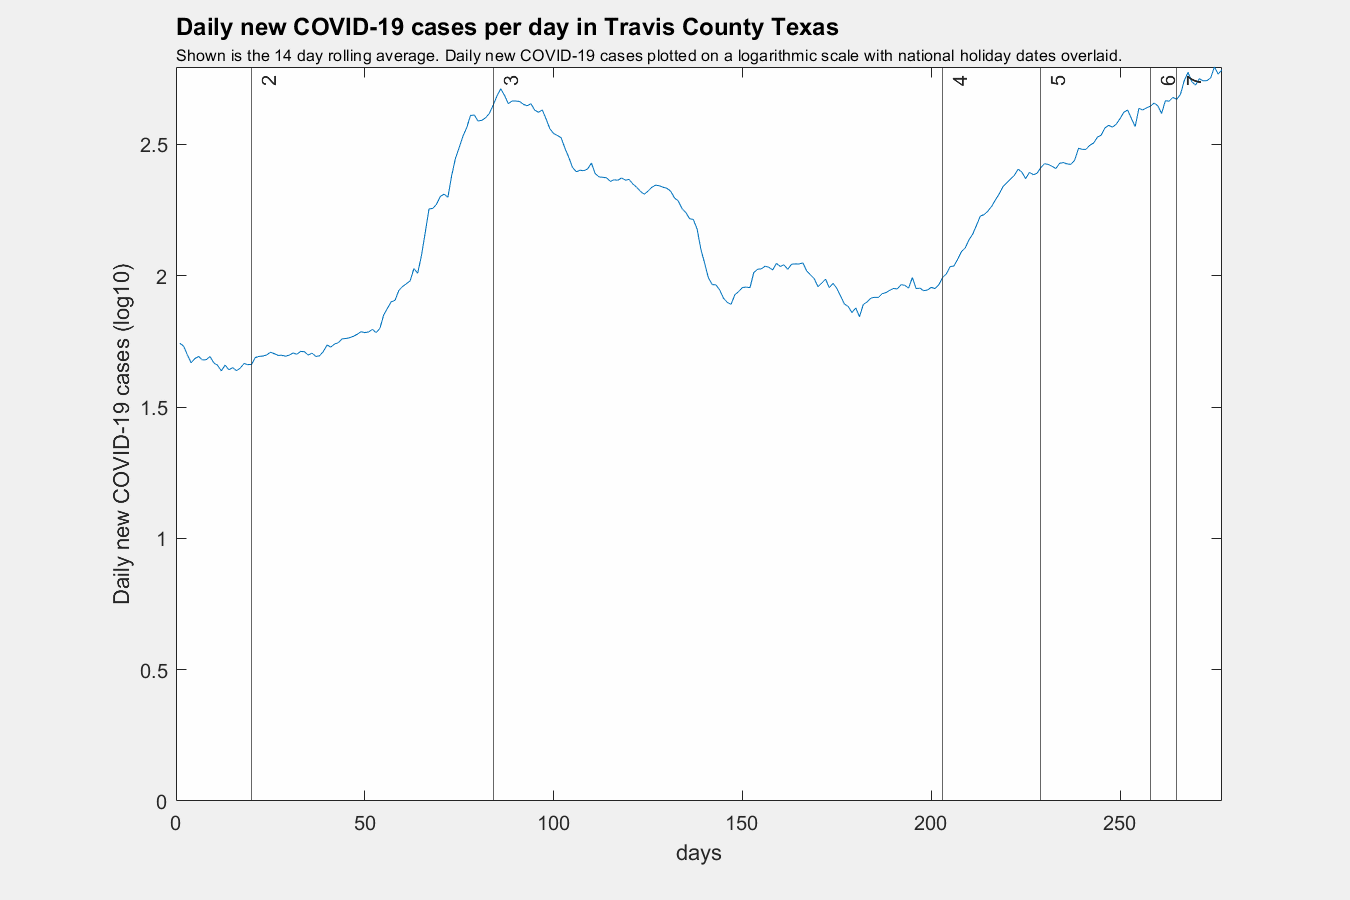
\includegraphics[width=\linewidth]{images/travis_cases_holiday_log.png}
	\caption{}
	\label{fig:images/travis_cases_holiday_logLabel}
\end{figure}

\begin{figure}[!h]
	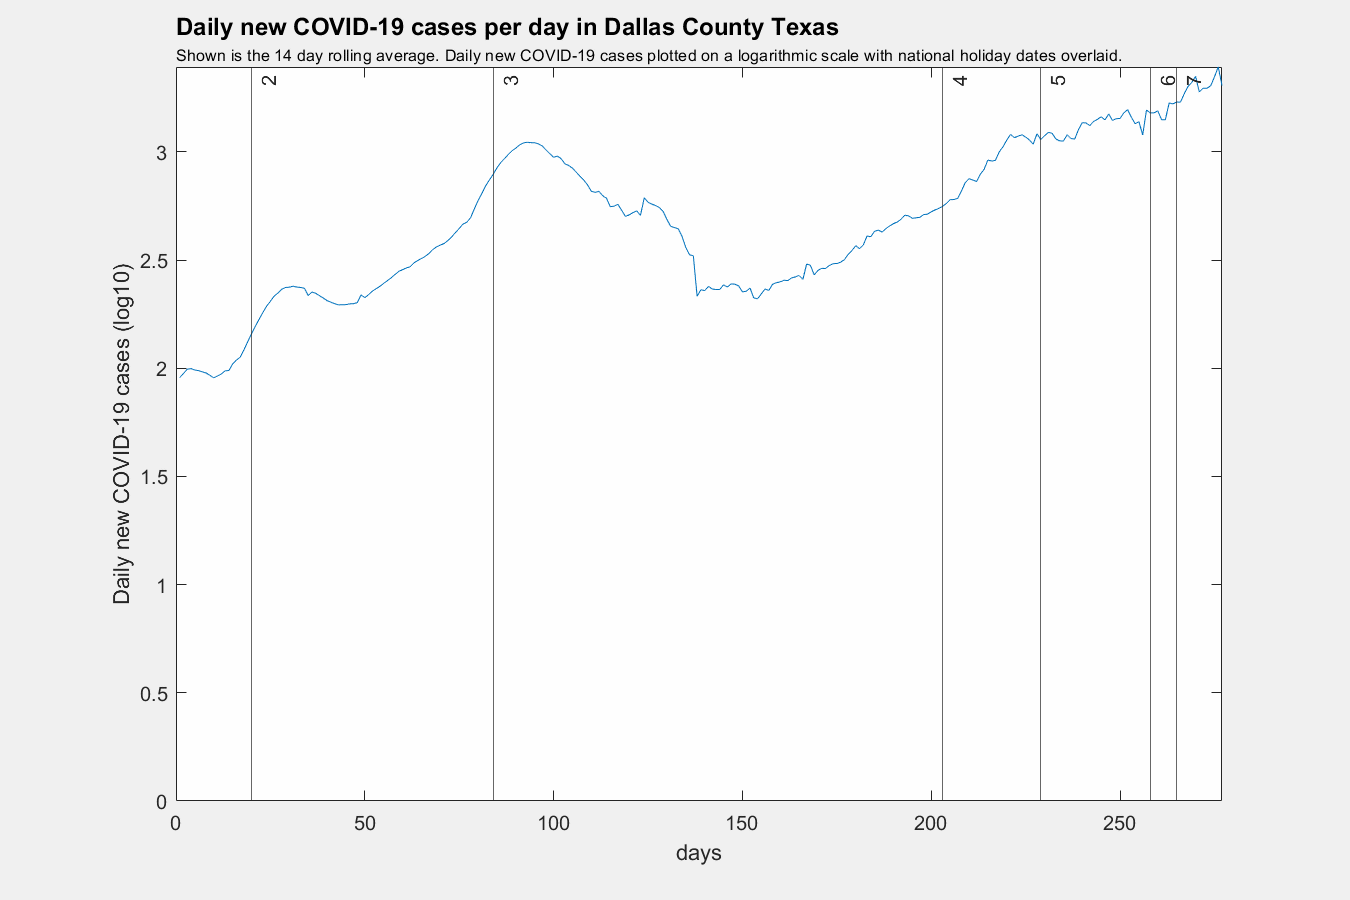
\includegraphics[width=\linewidth]{images/dallas_cases_holiday_log.png}
	\caption{}
	\label{fig:images/dallas_cases_holiday_logLabel}
\end{figure}

\begin{figure}[!h]
	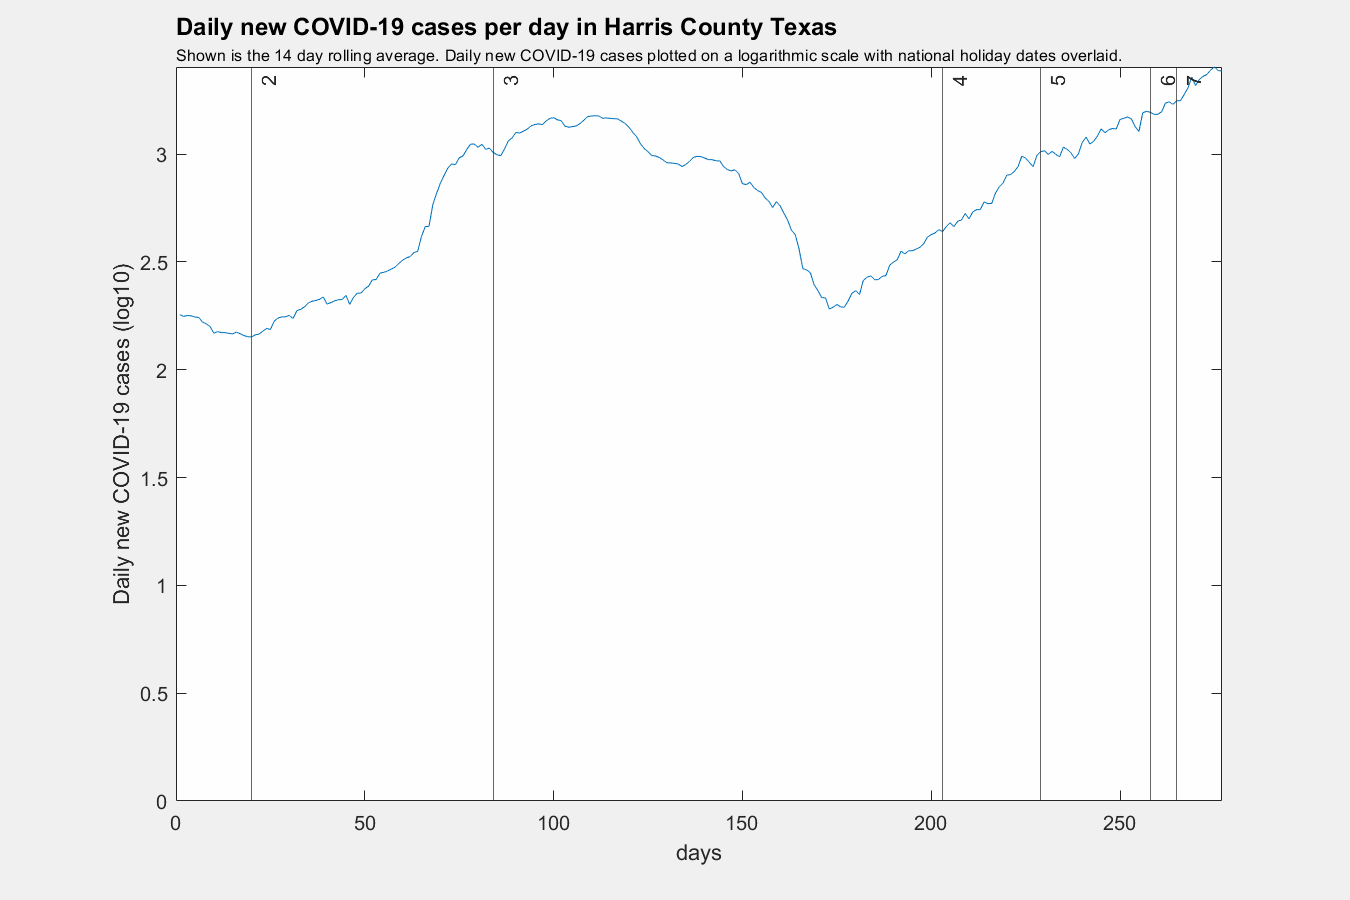
\includegraphics[width=\linewidth]{images/harris_cases_holiday_log.png}
	\caption{}
	\label{fig:images/harris_cases_holiday_logLabel}
\end{figure}

\FloatBarrier

In figures 32-40, the 14 day moving average of daily new COVID-19 cases per day in 9 counties is displayed on a logarithmic scale ($log_{10}$) with vertical line overlays representing the dates of several national and seasonal holidays have occurred. The counties assessed are Miami-Dade County, Florida; Broward County, Florida; Orange County, Florida; Los Angeles County, California; San Bernardino County, California; San Francisco County, California; Travis County, Texas; Dallas County, Texas; and Harris County, Texas. The genomic isolation dates of the COVID-19 variant strains in figures 22-30 are belonging to: CAL.20C (of lineage B.1.429), first isolated in California; B.1.1.207, first isolated in Nigeria; B.1.1.7 (aka VOC-202012/01, and as lineage B.1.1.7, or 20I/501Y.V1), first isolated in the United Kingdom; B.1.351 (aka 20H/501Y.V2, formerly known as 20C/501Y.V2), first isolated in South Africa; and P.1 (of lineage B.1.1.248), first isolated in Tokyo, and colloquially referred to as the Brazilian variant.


\FloatBarrier
\vspace{5mm}

\section*{The post-holiday surge; holidays and daily new COVID-19  hospitalizations}

\begin{figure}[!h]
	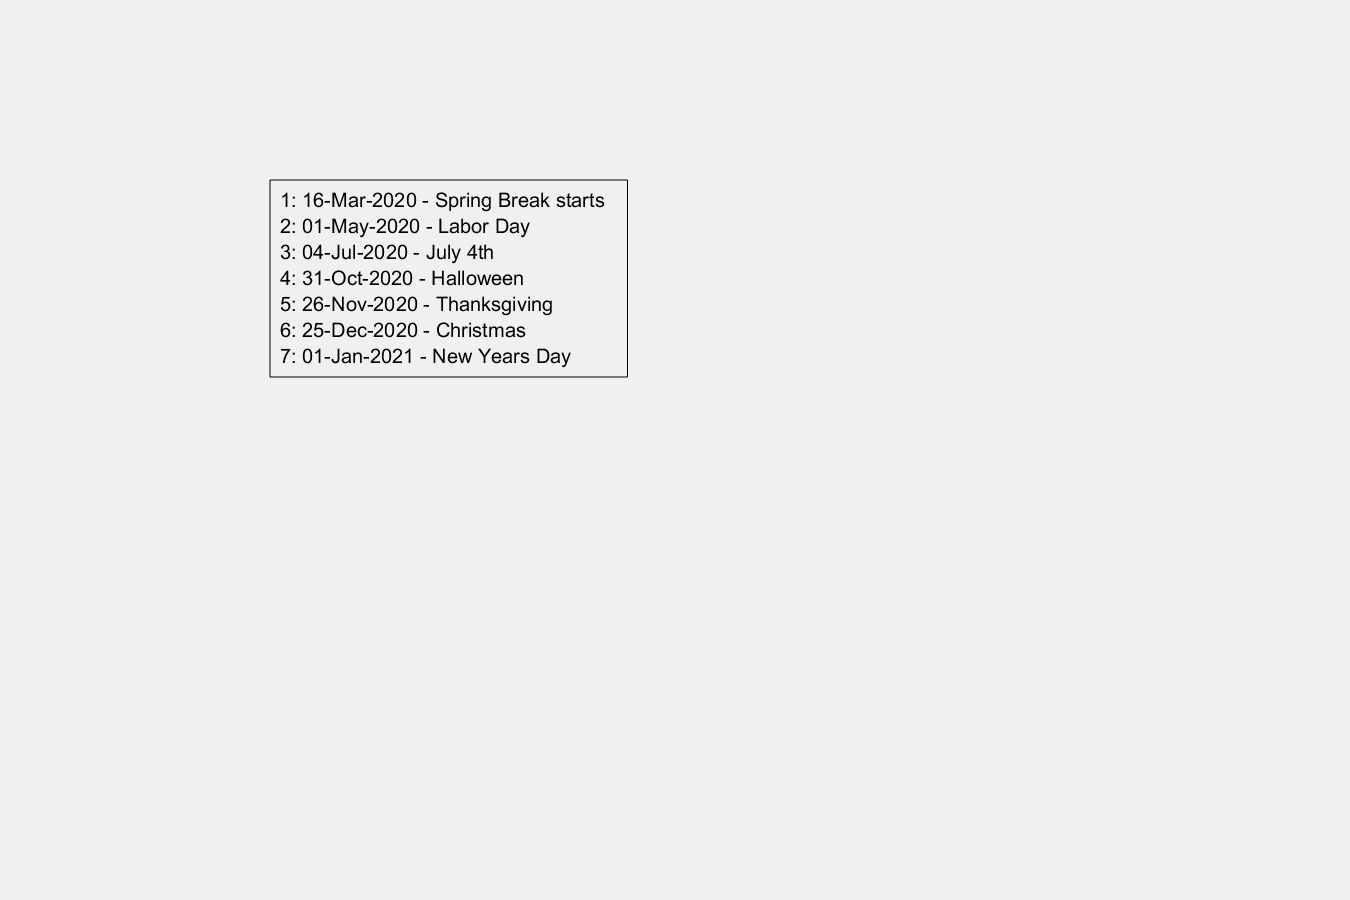
\includegraphics[width=\linewidth]{legends/holiday_legend.png}
	\caption{}
	\label{fig:legends/holiday_legendLabel}
\end{figure}

\begin{figure}[!h]
	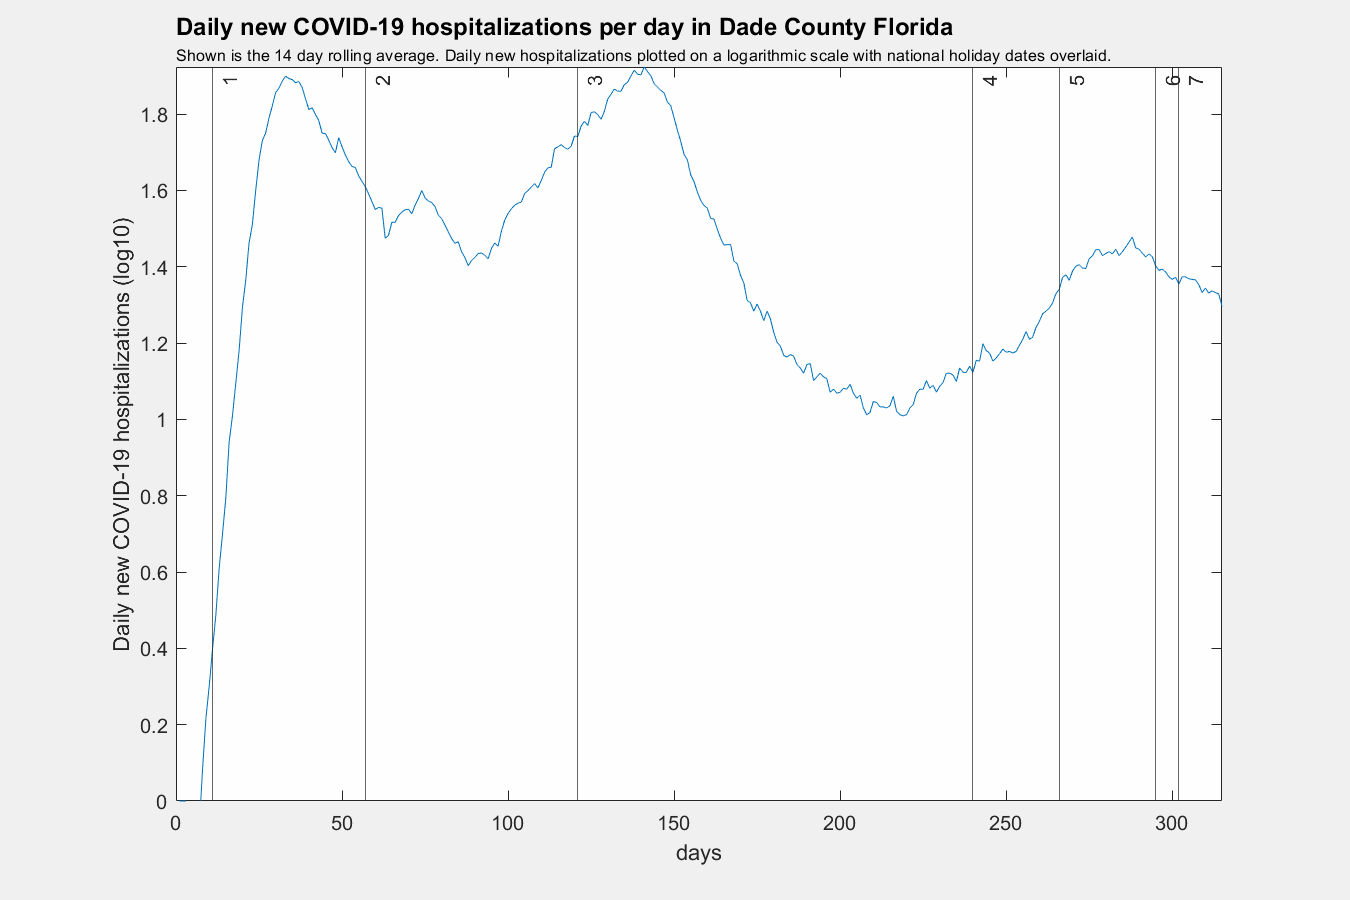
\includegraphics[width=\linewidth]{images/dade_hospitalizations_holiday_log.png}
	\caption{}
	\label{fig:images/dade_hospitalizations_holiday_logLabel}
\end{figure}

\begin{figure}[!h]
	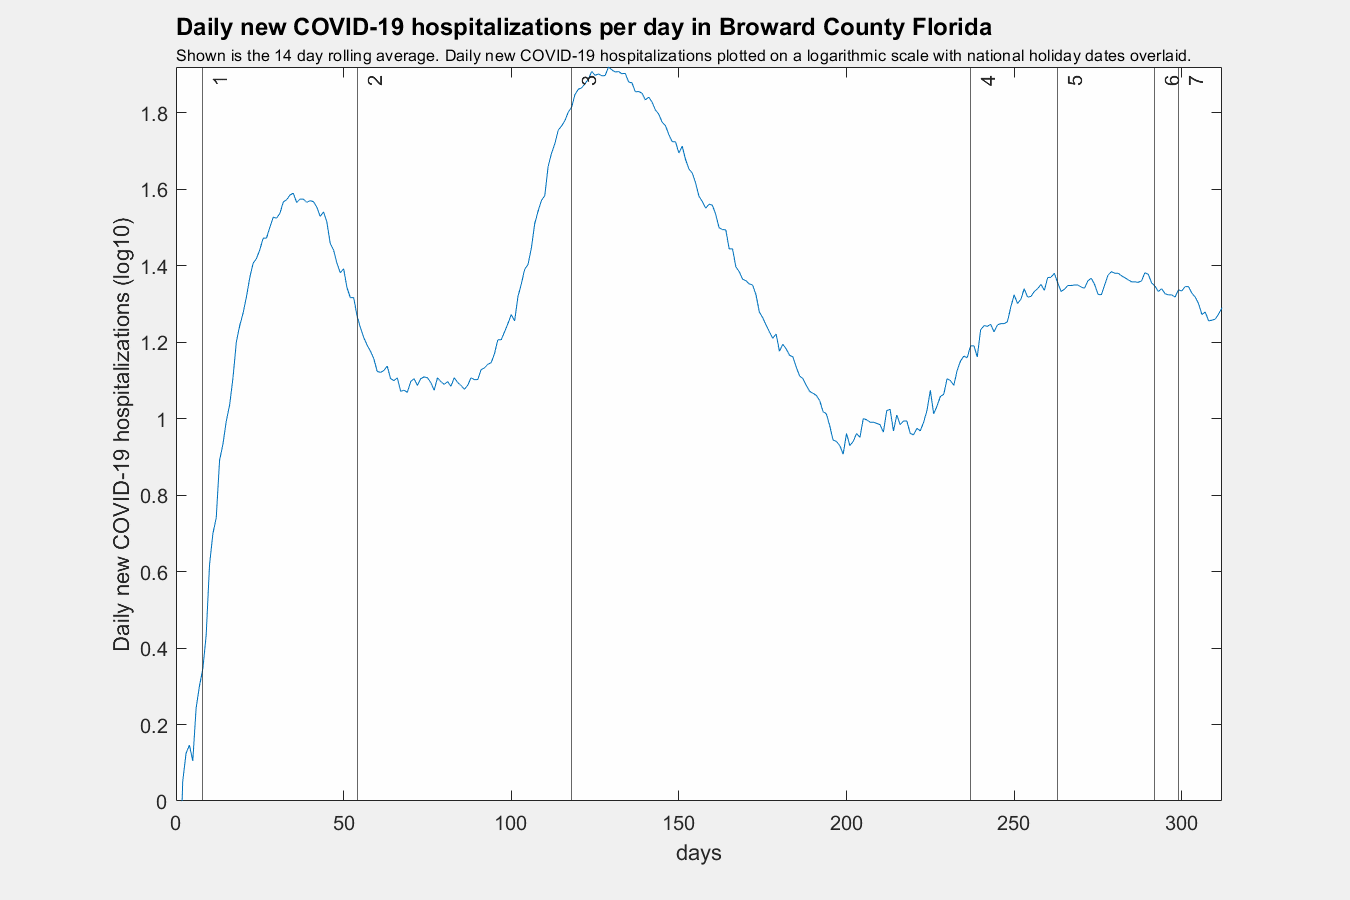
\includegraphics[width=\linewidth]{images/broward_hospitalizations_holiday_log.png}
	\caption{}
	\label{fig:images/broward_hospitalizations_holiday_logLabel}
\end{figure}

\begin{figure}[!h]
	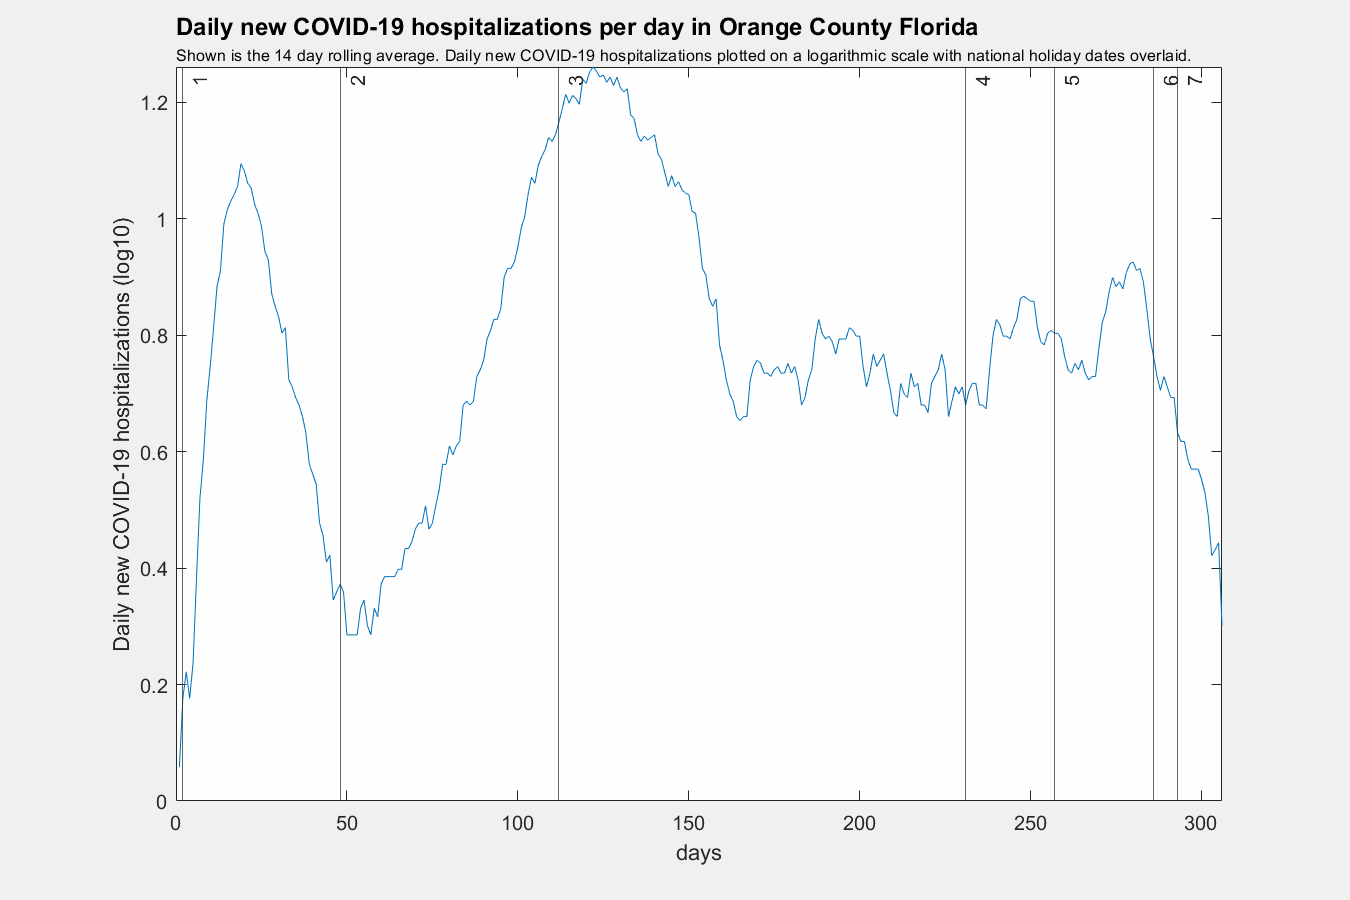
\includegraphics[width=\linewidth]{images/orange_hospitalizations_holiday_log.png}
	\caption{}
	\label{fig:images/orange_hospitalizations_holiday_logLabel}
\end{figure}

\begin{figure}[!h]
	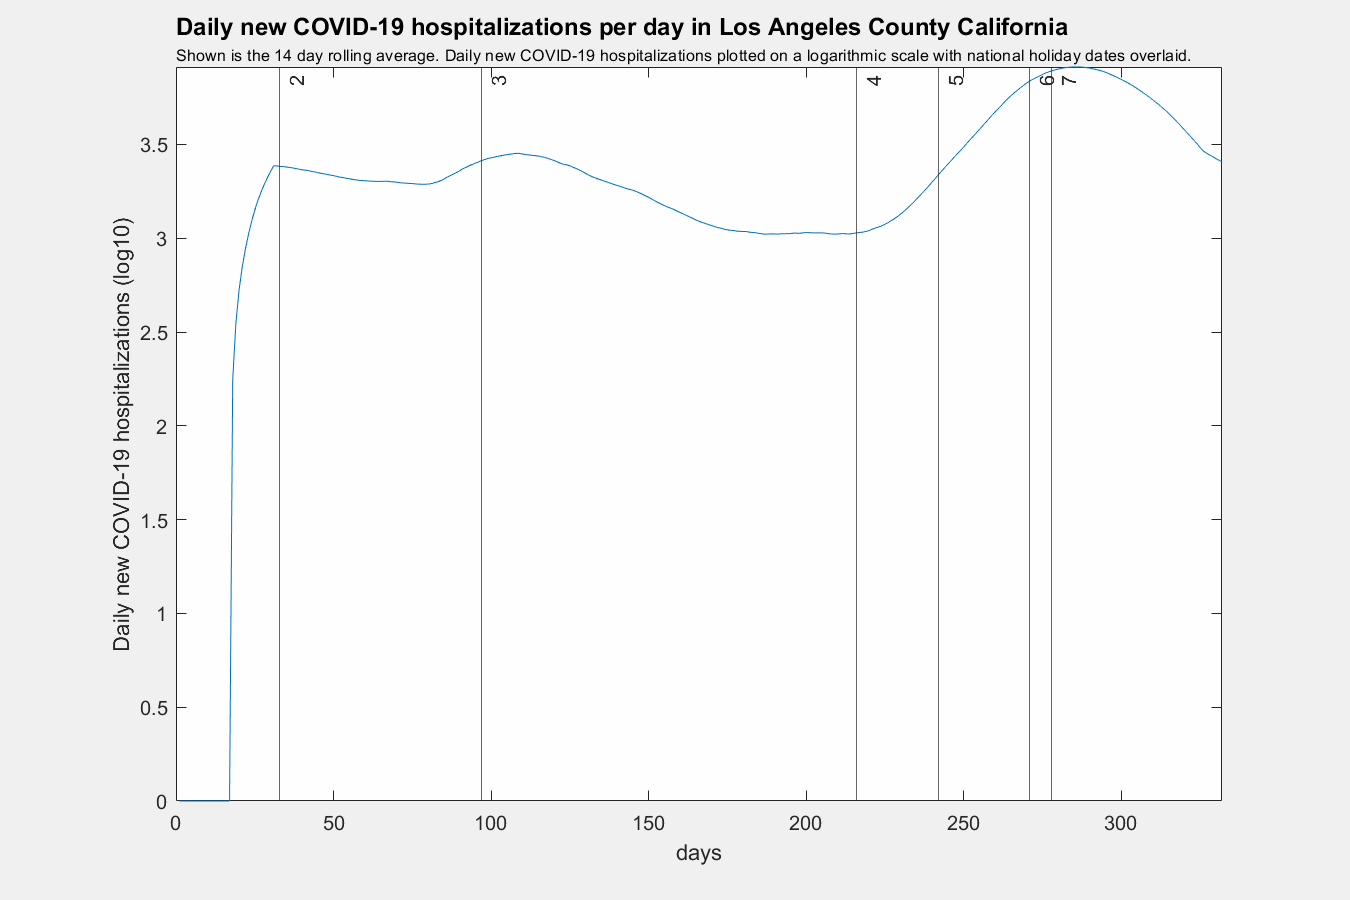
\includegraphics[width=\linewidth]{images/los_angeles_hospitalizations_holiday_log.png}
	\caption{}
	\label{fig:images/los_angeles_hospitalizations_holiday_logLabel}
\end{figure}

\begin{figure}[!h]
	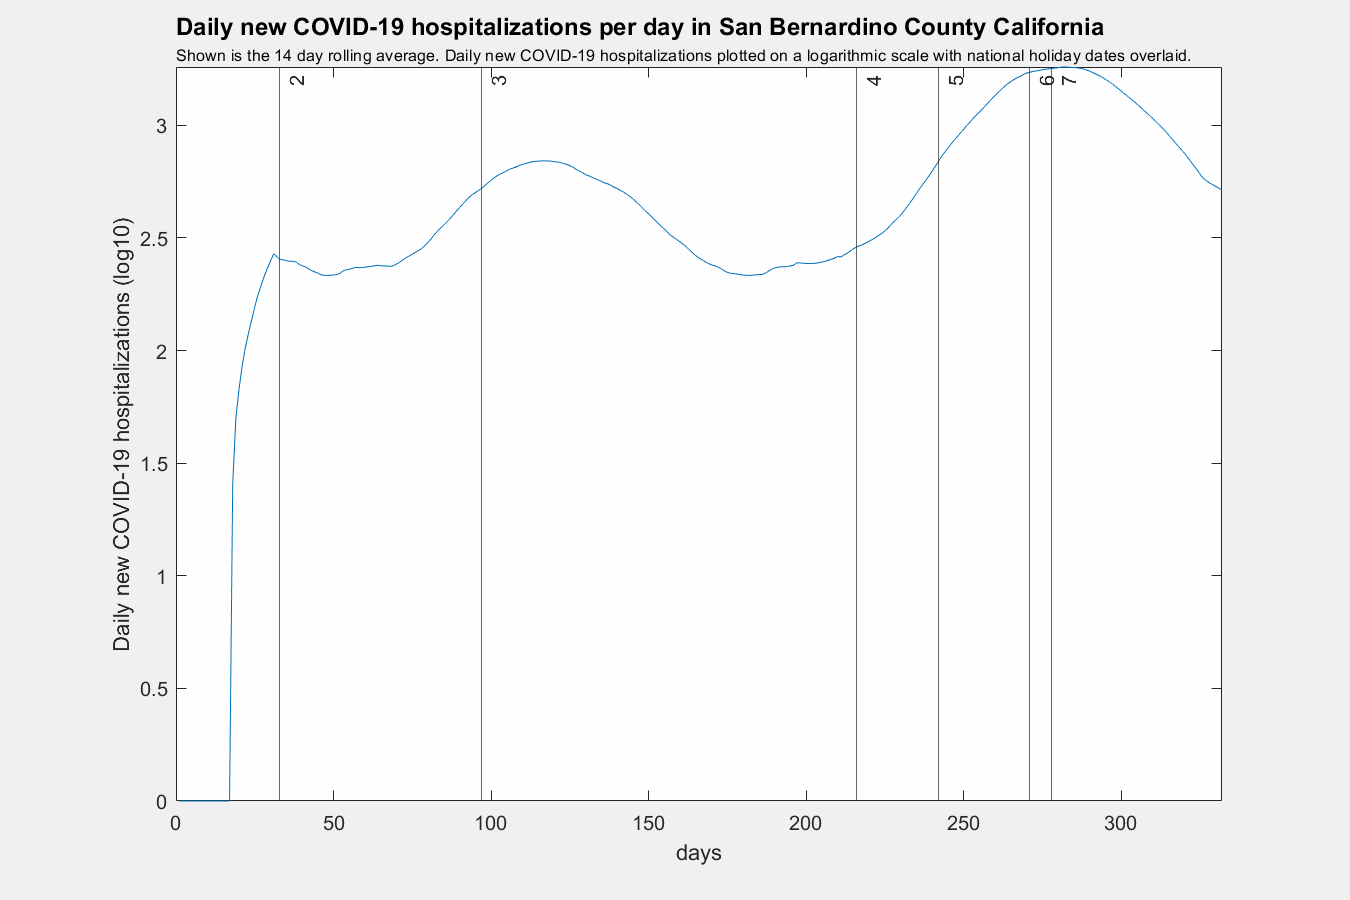
\includegraphics[width=\linewidth]{images/san_bernardino_hospitalizations_holiday_log.png}
	\caption{}
	\label{fig:images/san_bernardino_hospitalizations_holiday_logLabel}
\end{figure}

\begin{figure}[!h]
	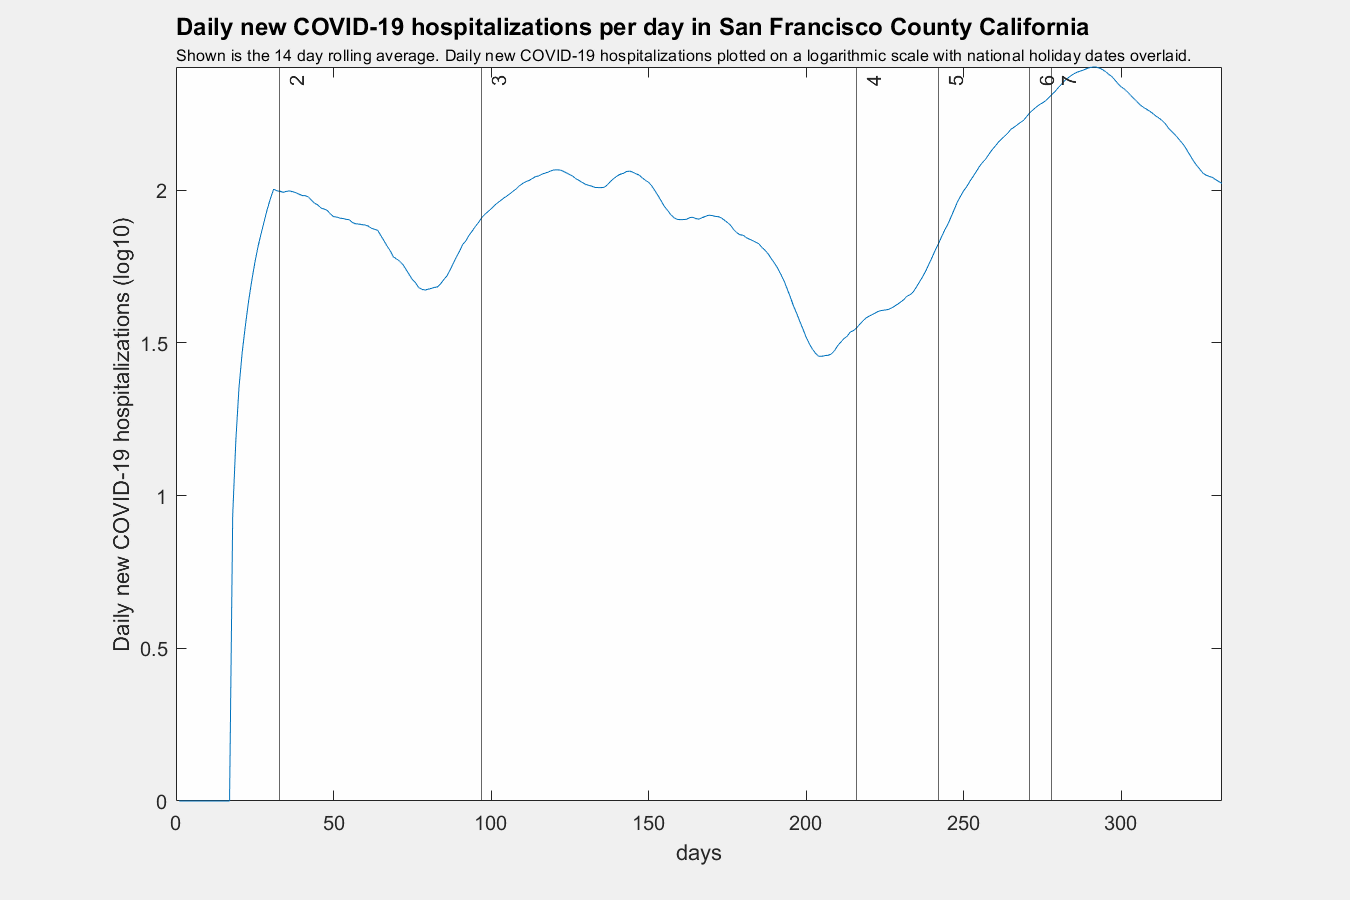
\includegraphics[width=\linewidth]{images/san_francisco_hospitalizations_holiday_log.png}
	\caption{}
	\label{fig:images/san_francisco_hospitalizations_holiday_logLabel}
\end{figure}

\begin{figure}[!h]
	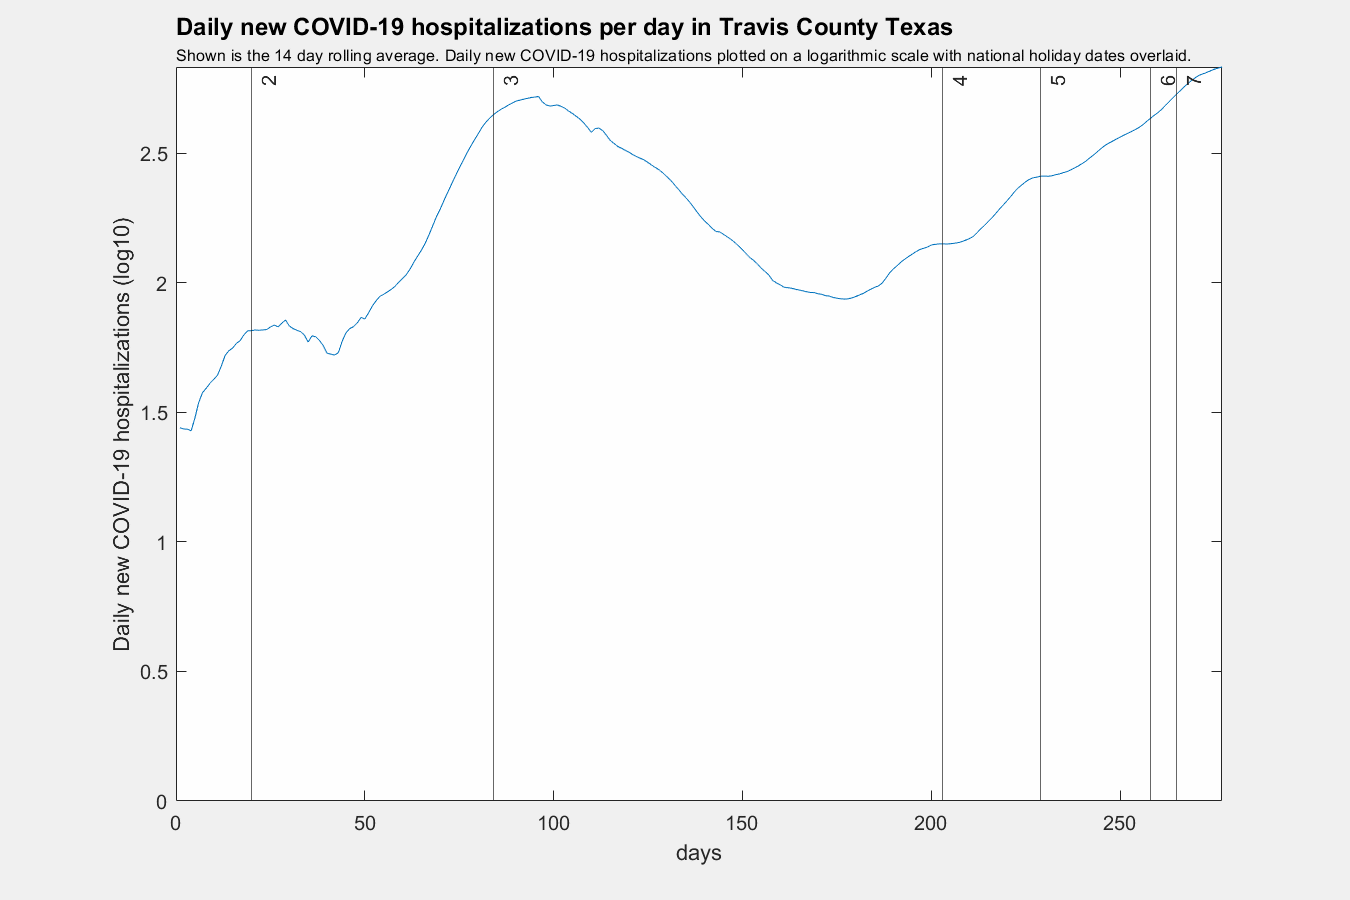
\includegraphics[width=\linewidth]{images/travis_hospitalizations_holiday_log.png}
	\caption{}
	\label{fig:images/travis_hospitalizations_holiday_logLabel}
\end{figure}

\begin{figure}[!h]
	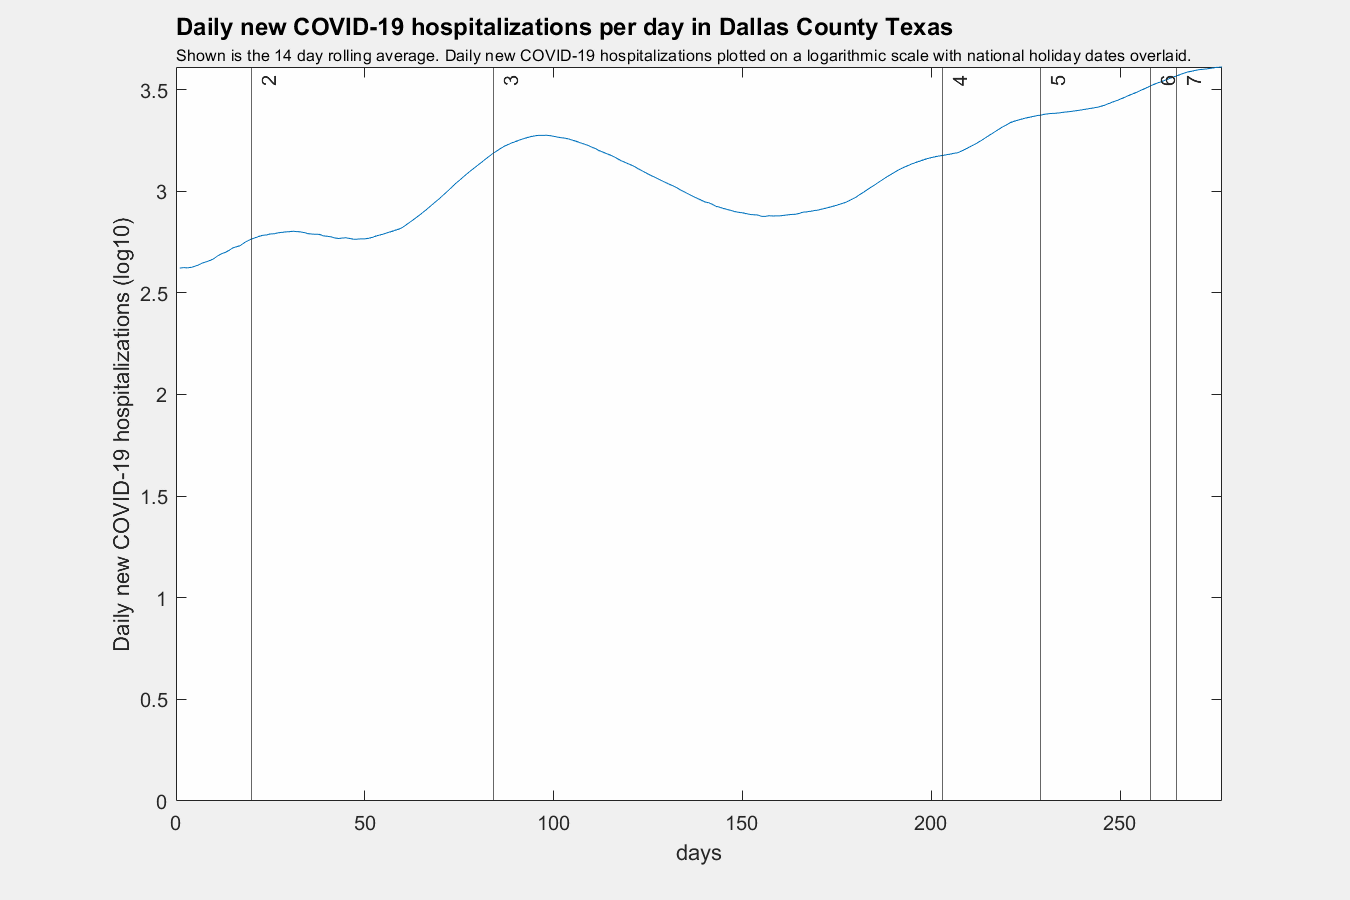
\includegraphics[width=\linewidth]{images/dallas_hospitalizations_holiday_log.png}
	\caption{}
	\label{fig:images/dallas_hospitalizations_holiday_logLabel}
\end{figure}

\begin{figure}[!h]
	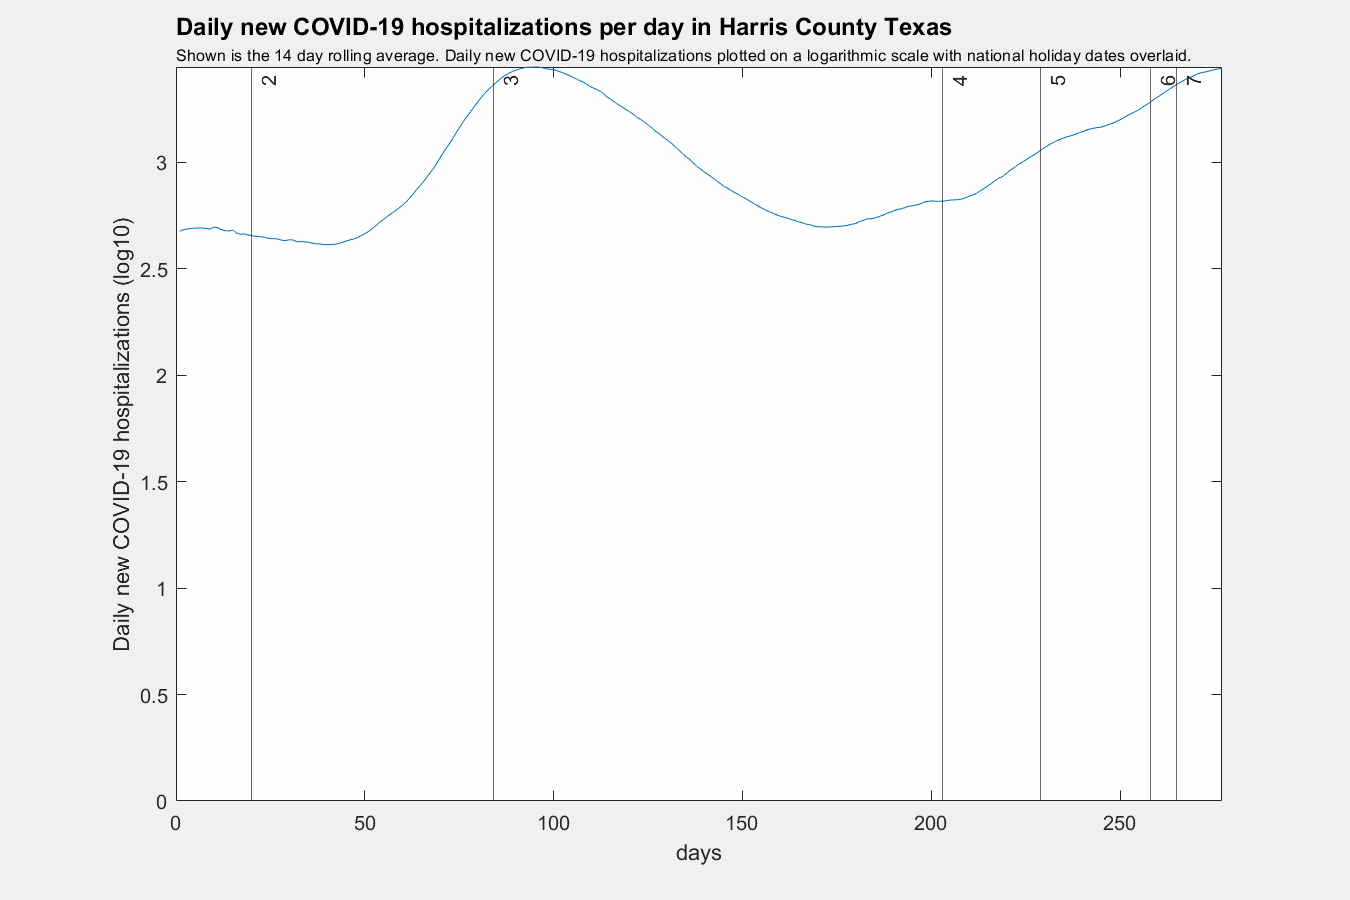
\includegraphics[width=\linewidth]{images/harris_hospitalizations_holiday_log.png}
	\caption{}
	\label{fig:images/harris_hospitalizations_holiday_logLabel}
\end{figure}

\FloatBarrier

In figures 42-50, the 14 day moving average of daily new COVID-19 hospitalizations per day in 9 counties is displayed on a logarithmic scale ($log_{10}$) with vertical line overlays representing the dates of several national and seasonal holidays have occurred. The counties assessed are Miami-Dade County, Florida; Broward County, Florida; Orange County, Florida; Los Angeles County, California; San Bernardino County, California; San Francisco County, California; Travis County, Texas; Dallas County, Texas; and Harris County, Texas. The genomic isolation dates of the COVID-19 variant strains in figures 22-30 are belonging to: CAL.20C (of lineage B.1.429), first isolated in California; B.1.1.207, first isolated in Nigeria; B.1.1.7 (aka VOC-202012/01, and as lineage B.1.1.7, or 20I/501Y.V1), first isolated in the United Kingdom; B.1.351 (aka 20H/501Y.V2, formerly known as 20C/501Y.V2), first isolated in South Africa; and P.1 (of lineage B.1.1.248), first isolated in Tokyo, and colloquially referred to as the Brazilian variant.


\FloatBarrier
\vspace{5mm}

\section*{The post-holiday surge; holidays and daily new COVID-19 fatalities}

\begin{figure}[!h]
	\includegraphics[width=\linewidth]{legends/holiday_legend.png}
	\caption{}
	\label{fig:legends/holiday_legendLabel}
\end{figure}

\begin{figure}[!h]
	\includegraphics[width=\linewidth]{images/dade_fatalities_holiday_log.png}
	\caption{}
	\label{fig:images/dade_fatalities_holiday_logLabel}
\end{figure}

\begin{figure}[!h]
	\includegraphics[width=\linewidth]{images/broward_fatalities_holiday_log.png}
	\caption{}
	\label{fig:images/broward_fatalities_holiday_logLabel}
\end{figure}

\begin{figure}[!h]
	\includegraphics[width=\linewidth]{images/orange_fatalities_holiday_log.png}
	\caption{}
	\label{fig:images/orange_fatalities_holiday_logLabel}
\end{figure}

\begin{figure}[!h]
	\includegraphics[width=\linewidth]{images/los_angeles_fatalities_holiday_log.png}
	\caption{}
	\label{fig:images/los_angeles_fatalities_holiday_logLabel}
\end{figure}

\begin{figure}[!h]
	\includegraphics[width=\linewidth]{images/san_bernardino_fatalities_holiday_log.png}
	\caption{}
	\label{fig:images/san_bernardino_fatalities_holiday_logLabel}
\end{figure}

\begin{figure}[!h]
	\includegraphics[width=\linewidth]{images/san_francisco_fatalities_holiday_log.png}
	\caption{}
	\label{fig:images/san_francisco_fatalities_holiday_logLabel}
\end{figure}

\begin{figure}[!h]
	\includegraphics[width=\linewidth]{images/travis_fatalities_holiday_log.png}
	\caption{}
	\label{fig:images/travis_fatalities_holiday_logLabel}
\end{figure}

\FloatBarrier

In figures 52-60, the 14 day moving average of daily new COVID-19 fatalities per day in 9 counties is displayed on a logarithmic scale ($log_{10}$) with vertical line overlays representing the dates of several national and seasonal holidays have occurred. The counties assessed are Miami-Dade County, Florida; Broward County, Florida; Orange County, Florida; Los Angeles County, California; San Bernardino County, California; San Francisco County, California; Travis County, Texas; Dallas County, Texas; and Harris County, Texas. The genomic isolation dates of the COVID-19 variant strains in figures 22-30 are belonging to: CAL.20C (of lineage B.1.429), first isolated in California; B.1.1.207, first isolated in Nigeria; B.1.1.7 (aka VOC-202012/01, and as lineage B.1.1.7, or 20I/501Y.V1), first isolated in the United Kingdom; B.1.351 (aka 20H/501Y.V2, formerly known as 20C/501Y.V2), first isolated in South Africa; and P.1 (of lineage B.1.1.248), first isolated in Tokyo, and colloquially referred to as the Brazilian variant.


\FloatBarrier
\vspace{5mm}
\section*{Government mask orders and the fluctuation in COVID-19 cases }

\begin{figure}[!h]
	\includegraphics[width=\linewidth]{legends/dade_mask_order_legend.png}
	\caption{}
	\label{fig:legends/dade_mask_order_legendLabel}
\end{figure}

\begin{figure}[!h]
	\includegraphics[width=\linewidth]{images/dade_mask_order_log.png}
	\caption{}
	\label{fig:images/dade_mask_order_logLabel}
\end{figure}

\begin{figure}[!h]
	\includegraphics[width=\linewidth]{legends/broward_mask_order_legend.png}
	\caption{}
	\label{fig:legends/broward_mask_order_legendLabel}
\end{figure}

\begin{figure}[!h]
	\includegraphics[width=\linewidth]{images/broward_mask_order_log.png}
	\caption{}
	\label{fig:images/broward_mask_order_logLabel}
\end{figure}

\begin{figure}[!h]
	\includegraphics[width=\linewidth]{legends/orange_mask_order_legend.png}
	\caption{}
	\label{fig:legends/orange_mask_order_legendLabel}
\end{figure}

\begin{figure}[!h]
	\includegraphics[width=\linewidth]{images/orange_mask_order_log.png}
	\caption{}
	\label{fig:images/orange_mask_order_logLabel}
\end{figure}


\begin{figure}[!h]
	\includegraphics[width=\linewidth]{legends/los_angeles_mask_order_legend.png}
	\caption{}
	\label{fig:legends/los_angeles_mask_order_legendLabel}
\end{figure}

\begin{figure}[!h]
	\includegraphics[width=\linewidth]{images/los_angeles_mask_order_log.png}
	\caption{}
	\label{fig:images/los_angeles_mask_order_logLabel}
\end{figure}


\begin{figure}[!h]
	\includegraphics[width=\linewidth]{legends/san_bernardino_mask_order_legend.png}
	\caption{}
	\label{fig:legends/san_bernardino_mask_order_legendLabel}
\end{figure}

\begin{figure}[!h]
	\includegraphics[width=\linewidth]{images/san_bernardino_mask_order_log.png}
	\caption{}
	\label{fig:images/san_bernardino_mask_order_logLabel}
\end{figure}

\begin{figure}[!h]
	\includegraphics[width=\linewidth]{legends/san_francisco_mask_order_legend.png}
	\caption{}
	\label{fig:legends/san_francisco_mask_order_legendLabel}
\end{figure}

\begin{figure}[!h]
	\includegraphics[width=\linewidth]{images/san_francisco_mask_order_log.png}
	\caption{}
	\label{fig:images/san_francisco_mask_order_logLabel}
\end{figure}

\begin{figure}[!h]
	\includegraphics[width=\linewidth]{legends/travis_mask_order_legend.png}
	\caption{}
	\label{fig:legends/travis_mask_order_legendLabel}
\end{figure}

\begin{figure}[!h]
	\includegraphics[width=\linewidth]{images/travis_mask_order_log.png}
	\caption{}
	\label{fig:images/travis_mask_order_logLabel}
\end{figure}

\begin{figure}[!h]
	\includegraphics[width=\linewidth]{legends/dallas_mask_order_legend.png}
	\caption{}
	\label{fig:legends/dallas_mask_order_legendLabel}
\end{figure}

\begin{figure}[!h]
	\includegraphics[width=\linewidth]{images/dallas_mask_order_log.png}
	\caption{}
	\label{fig:images/dallas_mask_order_logLabel}
\end{figure}

\begin{figure}[!h]
	\includegraphics[width=\linewidth]{legends/harris_mask_order_legend.png}
	\caption{}
	\label{fig:legends/harris_mask_order_legendLabel}
\end{figure}

\begin{figure}[!h]
	\includegraphics[width=\linewidth]{images/harris_mask_order_log.png}
	\caption{}
	\label{fig:images/harris_mask_order_logLabel}
\end{figure}

\FloatBarrier

In figures XX-XX, the 14 day moving average of daily new COVID-19 cases per day in 9 counties is displayed on a logarithmic scale ($log_{10}$) with vertical line overlays representing the dates in which local and state mask order dates were initiated. The counties assessed are Miami-Dade County, Florida; Broward County, Florida; Orange County, Florida; Los Angeles County, California; San Bernardino County, California; San Francisco County, California; Travis County, Texas; Dallas County, Texas; and Harris County, Texas. The genomic isolation dates of the COVID-19 variant strains in figures 22-30 are belonging to: CAL.20C (of lineage B.1.429), first isolated in California; B.1.1.207, first isolated in Nigeria; B.1.1.7 (aka VOC-202012/01, and as lineage B.1.1.7, or 20I/501Y.V1), first isolated in the United Kingdom; B.1.351 (aka 20H/501Y.V2, formerly known as 20C/501Y.V2), first isolated in South Africa; and P.1 (of lineage B.1.1.248), first isolated in Tokyo, and colloquially referred to as the Brazilian variant.


\FloatBarrier

\vspace{5mm}
\section*{Government mask orders and the fluctuation in COVID-19 hospitalizations }


\begin{figure}[!h]
	\includegraphics[width=\linewidth]{legends/dade_mask_order_legend.png}
	\caption{}
	\label{fig:legends/dade_mask_order_legendLabel}
\end{figure}

\begin{figure}[!h]
	\includegraphics[width=\linewidth]{images/dade_mask_order_hospitalizations_log.png}
	\caption{}
	\label{fig:images/dade_mask_order_hospitalizations_logLabel}
\end{figure}

\begin{figure}[!h]
	\includegraphics[width=\linewidth]{legends/broward_mask_order_legend.png}
	\caption{}
	\label{fig:legends/broward_mask_order_legendLabel}
\end{figure}

\begin{figure}[!h]
	\includegraphics[width=\linewidth]{images/broward_mask_order_hospitalizations_log.png}
	\caption{}
	\label{fig:images/broward_mask_order_hospitalizations_logLabel}
\end{figure}

\begin{figure}[!h]
	\includegraphics[width=\linewidth]{legends/orange_mask_order_legend.png}
	\caption{}
	\label{fig:legends/orange_mask_order_legendLabel}
\end{figure}

\begin{figure}[!h]
	\includegraphics[width=\linewidth]{images/orange_mask_order_hospitalizations_log.png}
	\caption{}
	\label{fig:images/orange_mask_order_hospitalizations_logLabel}
\end{figure}

\begin{figure}[!h]
	\includegraphics[width=\linewidth]{legends/los_angeles_mask_order_legend.png}
	\caption{}
	\label{fig:legends/los_angeles_mask_order_legendLabel}
\end{figure}

\begin{figure}[!h]
	\includegraphics[width=\linewidth]{images/los_angeles_mask_order_hospitalizations_log.png}
	\caption{}
	\label{fig:images/los_angeles_mask_order_hospitalizations_logLabel}
\end{figure}

\begin{figure}[!h]
	\includegraphics[width=\linewidth]{legends/san_bernardino_mask_order_legend.png}
	\caption{}
	\label{fig:legends/san_bernardino_mask_order_legendLabel}
\end{figure}

\begin{figure}[!h]
	\includegraphics[width=\linewidth]{images/san_bernardino_mask_order_hospitalizations_log.png}
	\caption{}
	\label{fig:images/san_bernardino_mask_order_hospitalizations_logLabel}
\end{figure}

\begin{figure}[!h]
	\includegraphics[width=\linewidth]{legends/san_francisco_mask_order_legend.png}
	\caption{}
	\label{fig:legends/san_francisco_mask_order_legendLabel}
\end{figure}

\begin{figure}[!h]
	\includegraphics[width=\linewidth]{images/san_francisco_mask_order_hospitalizations_log.png}
	\caption{}
	\label{fig:images/san_francisco_mask_order_hospitalizations_logLabel}
\end{figure}


\begin{figure}[!h]
	\includegraphics[width=\linewidth]{legends/travis_mask_order_legend.png}
	\caption{}
	\label{fig:legends/travis_mask_order_legendLabel}
\end{figure}

\begin{figure}[!h]
	\includegraphics[width=\linewidth]{images/travis_mask_order_hospitalizations_log.png}
	\caption{}
	\label{fig:images/travis_mask_order_hospitalizations_logLabel}
\end{figure}

\begin{figure}[!h]
	\includegraphics[width=\linewidth]{legends/dallas_mask_order_legend.png}
	\caption{}
	\label{fig:legends/dallas_mask_order_legendLabel}
\end{figure}

\begin{figure}[!h]
	\includegraphics[width=\linewidth]{images/dallas_mask_order_hospitalizations_log.png}
	\caption{}
	\label{fig:images/dallas_mask_order_hospitalizations_logLabel}
\end{figure}


\begin{figure}[!h]
	\includegraphics[width=\linewidth]{legends/harris_mask_order_legend.png}
	\caption{}
	\label{fig:legends/harris_mask_order_legendLabel}
\end{figure}


\begin{figure}[!h]
	\includegraphics[width=\linewidth]{images/harris_mask_order_hospitalizations_log.png}
	\caption{}
	\label{fig:images/harris_mask_order_hospitalizations_logLabel}
\end{figure}

\FloatBarrier

In figures XX-XX, the 14 day moving average of daily new COVID-19 hospitalizations per day in 9 counties is displayed on a logarithmic scale ($log_{10}$) with vertical line overlays representing the dates in which local and state mask order dates were initiated. The counties assessed are Miami-Dade County, Florida; Broward County, Florida; Orange County, Florida; Los Angeles County, California; San Bernardino County, California; San Francisco County, California; Travis County, Texas; Dallas County, Texas; and Harris County, Texas. The genomic isolation dates of the COVID-19 variant strains in figures 22-30 are belonging to: CAL.20C (of lineage B.1.429), first isolated in California; B.1.1.207, first isolated in Nigeria; B.1.1.7 (aka VOC-202012/01, and as lineage B.1.1.7, or 20I/501Y.V1), first isolated in the United Kingdom; B.1.351 (aka 20H/501Y.V2, formerly known as 20C/501Y.V2), first isolated in South Africa; and P.1 (of lineage B.1.1.248), first isolated in Tokyo, and colloquially referred to as the Brazilian variant.

\FloatBarrier

\vspace{5mm}
\section*{Government mask orders and the fluctuation in COVID-19 fatalities }

\begin{figure}[!h]
	\includegraphics[width=\linewidth]{legends/dade_mask_order_legend.png}
	\caption{}
	\label{fig:legends/dade_mask_order_legendLabel}
\end{figure}

\begin{figure}[!h]
	\includegraphics[width=\linewidth]{images/dade_mask_order_fatalities_log.png}
	\caption{}
	\label{fig:images/dade_mask_order_fatalities_logLabel}
\end{figure}

\begin{figure}[!h]
	\includegraphics[width=\linewidth]{legends/broward_mask_order_legend.png}
	\caption{}
	\label{fig:legends/broward_mask_order_legendLabel}
\end{figure}

\begin{figure}[!h]
	\includegraphics[width=\linewidth]{images/broward_mask_order_fatalities_log.png}
	\caption{}
	\label{fig:images/broward_mask_order_fatalities_logLabel}
\end{figure}

\begin{figure}[!h]
	\includegraphics[width=\linewidth]{legends/orange_mask_order_legend.png}
	\caption{}
	\label{fig:legends/orange_mask_order_legendLabel}
\end{figure}

\begin{figure}[!h]
	\includegraphics[width=\linewidth]{images/orange_mask_order_fatalities_log.png}
	\caption{}
	\label{fig:images/orange_mask_order_fatalities_logLabel}
\end{figure}

\begin{figure}[!h]
	\includegraphics[width=\linewidth]{legends/los_angeles_mask_order_legend.png}
	\caption{}
	\label{fig:legends/los_angeles_mask_order_legendLabel}
\end{figure}

\begin{figure}[!h]
	\includegraphics[width=\linewidth]{images/los_angeles_mask_order_fatalities_log.png}
	\caption{}
	\label{fig:images/los_angeles_mask_order_fatalities_logLabel}
\end{figure}

\begin{figure}[!h]
	\includegraphics[width=\linewidth]{legends/san_bernardino_mask_order_legend.png}
	\caption{}
	\label{fig:legends/san_bernardino_mask_order_legendLabel}
\end{figure}

\begin{figure}[!h]
	\includegraphics[width=\linewidth]{images/san_bernardino_mask_order_fatalities_log.png}
	\caption{}
	\label{fig:images/san_bernardino_mask_order_fatalities_logLabel}
\end{figure}

\begin{figure}[!h]
	\includegraphics[width=\linewidth]{legends/san_francisco_mask_order_legend.png}
	\caption{}
	\label{fig:legends/san_francisco_mask_order_legendLabel}
\end{figure}

\begin{figure}[!h]
	\includegraphics[width=\linewidth]{images/san_francisco_mask_order_fatalities_log.png}
	\caption{}
	\label{fig:images/san_francisco_mask_order_fatalities_logLabel}
\end{figure}

\begin{figure}[!h]
	\includegraphics[width=\linewidth]{legends/travis_mask_order_legend.png}
	\caption{}
	\label{fig:legends/travis_mask_order_legendLabel}
\end{figure}

\begin{figure}[!h]
	\includegraphics[width=\linewidth]{images/travis_mask_order_fatalities_log.png}
	\caption{}
	\label{fig:images/travis_mask_order_fatalities_logLabel}
\end{figure}

\begin{figure}[!h]
	\includegraphics[width=\linewidth]{legends/dallas_mask_order_legend.png}
	\caption{}
	\label{fig:legends/dallas_mask_order_legendLabel}
\end{figure}

\begin{figure}[!h]
	\includegraphics[width=\linewidth]{images/dallas_mask_order_fatalities_log.png}
	\caption{}
	\label{fig:images/dallas_mask_order_fatalities_logLabel}
\end{figure}

\begin{figure}[!h]
	\includegraphics[width=\linewidth]{legends/harris_mask_order_legend.png}
	\caption{}
	\label{fig:legends/harris_mask_order_legendLabel}
\end{figure}

\begin{figure}[!h]
	\includegraphics[width=\linewidth]{images/harris_mask_order_fatalities_log.png}
	\caption{}
	\label{fig:images/harris_mask_order_fatalities_logLabel}
\end{figure}

\FloatBarrier

In figures XX-XX, the 14 day moving average of daily new COVID-19 fatalities per day in 9 counties is displayed on a logarithmic scale ($log_{10}$) with vertical line overlays representing the dates in which local and state mask order dates were initiated. The counties assessed are Miami-Dade County, Florida; Broward County, Florida; Orange County, Florida; Los Angeles County, California; San Bernardino County, California; San Francisco County, California; Travis County, Texas; Dallas County, Texas; and Harris County, Texas. The genomic isolation dates of the COVID-19 variant strains in figures 22-30 are belonging to: CAL.20C (of lineage B.1.429), first isolated in California; B.1.1.207, first isolated in Nigeria; B.1.1.7 (aka VOC-202012/01, and as lineage B.1.1.7, or 20I/501Y.V1), first isolated in the United Kingdom; B.1.351 (aka 20H/501Y.V2, formerly known as 20C/501Y.V2), first isolated in South Africa; and P.1 (of lineage B.1.1.248), first isolated in Tokyo, and colloquially referred to as the Brazilian variant.

\FloatBarrier
\vspace{5mm}
\section*{School closings, re-openings and daily new COVID-19 cases  }

\begin{figure}[!h]
	\includegraphics[width=\linewidth]{legends/dade_school_legend.png}
	\caption{}
	\label{fig:legends/dade_school_legendLabel}
\end{figure}

\begin{figure}[!h]
	\includegraphics[width=\linewidth]{images/dade_cases_school_log.png}
	\caption{}
	\label{fig:images/dade_cases_school_logLabel}
\end{figure}

\begin{figure}[!h]
	\includegraphics[width=\linewidth]{legends/broward_school_legend.png}
	\caption{}
	\label{fig:legends/broward_school_legendLabel}
\end{figure}

\begin{figure}[!h]
	\includegraphics[width=\linewidth]{images/broward_cases_school_log.png}
	\caption{}
	\label{fig:images/broward_cases_school_logLabel}
\end{figure}

\begin{figure}[!h]
	\includegraphics[width=\linewidth]{legends/orange_school_legend.png}
	\caption{}
	\label{fig:legends/orange_school_legendLabel}
\end{figure}

\begin{figure}[!h]
	\includegraphics[width=\linewidth]{images/orange_cases_school_log.png}
	\caption{}
	\label{fig:images/orange_cases_school_logLabel}
\end{figure}

\begin{figure}[!h]
	\includegraphics[width=\linewidth]{legends/los_angeles_school_legend.png}
	\caption{}
	\label{fig:legends/los_angeles_school_legendLabel}
\end{figure}

\begin{figure}[!h]
	\includegraphics[width=\linewidth]{images/los_angeles_cases_school_log.png}
	\caption{}
	\label{fig:images/los_angeles_cases_school_logLabel}
\end{figure}

\begin{figure}[!h]
	\includegraphics[width=\linewidth]{legends/san_bernardino_school_legend.png}
	\caption{}
	\label{fig:legends/san_bernardino_school_legendLabel}
\end{figure}

\begin{figure}[!h]
	\includegraphics[width=\linewidth]{images/san_bernardino_cases_school_log.png}
	\caption{}
	\label{fig:images/san_bernardino_cases_school_logLabel}
\end{figure}

\begin{figure}[!h]
	\includegraphics[width=\linewidth]{legends/san_francisco_school_legend.png}
	\caption{}
	\label{fig:legends/san_francisco_school_legendLabel}
\end{figure}

\begin{figure}[!h]
	\includegraphics[width=\linewidth]{images/san_francisco_cases_school_log.png}
	\caption{}
	\label{fig:images/san_francisco_cases_school_logLabel}
\end{figure}

\begin{figure}[!h]
	\includegraphics[width=\linewidth]{legends/travis_school_legend.png}
	\caption{}
	\label{fig:legends/travis_school_legendLabel}
\end{figure}

\begin{figure}[!h]
	\includegraphics[width=\linewidth]{images/travis_cases_school_log.png}
	\caption{}
	\label{fig:images/travis_cases_school_logLabel}
\end{figure}

\begin{figure}[!h]
	\includegraphics[width=\linewidth]{legends/dallas_school_legend.png}
	\caption{}
	\label{fig:legends/dallas_school_legendLabel}
\end{figure}

\begin{figure}[!h]
	\includegraphics[width=\linewidth]{images/dallas_cases_school_log.png}
	\caption{}
	\label{fig:images/dallas_cases_school_logLabel}
\end{figure}

\begin{figure}[!h]
	\includegraphics[width=\linewidth]{legends/harris_school_legend.png}
	\caption{}
	\label{fig:legends/harris_school_legendLabel}
\end{figure}

\begin{figure}[!h]
	\includegraphics[width=\linewidth]{images/harris_cases_school_log.png}
	\caption{}
	\label{fig:images/harris_cases_school_logLabel}
\end{figure}


\FloatBarrier

In figures XX-XX, the 14 day moving average of daily new COVID-19 cases per day in 9 counties is displayed on a logarithmic scale ($log_{10}$) with vertical line overlays representing the dates in which local school openings and closings have occurred. The counties assessed are Miami-Dade County, Florida; Broward County, Florida; Orange County, Florida; Los Angeles County, California; San Bernardino County, California; San Francisco County, California; Travis County, Texas; Dallas County, Texas; and Harris County, Texas. The genomic isolation dates of the COVID-19 variant strains in figures 22-30 are belonging to: CAL.20C (of lineage B.1.429), first isolated in California; B.1.1.207, first isolated in Nigeria; B.1.1.7 (aka VOC-202012/01, and as lineage B.1.1.7, or 20I/501Y.V1), first isolated in the United Kingdom; B.1.351 (aka 20H/501Y.V2, formerly known as 20C/501Y.V2), first isolated in South Africa; and P.1 (of lineage B.1.1.248), first isolated in Tokyo, and colloquially referred to as the Brazilian variant.



\FloatBarrier
\vspace{5mm}
\section*{School closings, re-openings and daily new COVID-19 hospitalizations }

\begin{figure}[!h]
	\includegraphics[width=\linewidth]{legends/dade_school_legend.png}
	\caption{}
	\label{fig:legends/dade_school_legendLabel}
\end{figure}

\begin{figure}[!h]
	\includegraphics[width=\linewidth]{images/dade_hospitalizations_school_log.png}
	\caption{}
	\label{fig:images/dade_hospitalizations_school_logLabel}
\end{figure}

\begin{figure}[!h]
	\includegraphics[width=\linewidth]{legends/broward_school_legend.png}
	\caption{}
	\label{fig:legends/broward_school_legendLabel}
\end{figure}

\begin{figure}[!h]
	\includegraphics[width=\linewidth]{images/broward_hospitalizations_school_log.png}
	\caption{}
	\label{fig:images/broward_hospitalizations_school_logLabel}
\end{figure}

\begin{figure}[!h]
	\includegraphics[width=\linewidth]{legends/orange_school_legend.png}
	\caption{}
	\label{fig:legends/orange_school_legendLabel}
\end{figure}

\begin{figure}[!h]
	\includegraphics[width=\linewidth]{images/orange_hospitalizations_school_log.png}
	\caption{}
	\label{fig:images/orange_hospitalizations_school_logLabel}
\end{figure}

\begin{figure}[!h]
	\includegraphics[width=\linewidth]{legends/los_angeles_school_legend.png}
	\caption{}
	\label{fig:legends/los_angeles_school_legendLabel}
\end{figure}

\begin{figure}[!h]
	\includegraphics[width=\linewidth]{images/los_angeles_hospitalizations_school_log.png}
	\caption{}
	\label{fig:images/los_angeles_hospitalizations_school_logLabel}
\end{figure}

\begin{figure}[!h]
	\includegraphics[width=\linewidth]{legends/san_bernardino_school_legend.png}
	\caption{}
	\label{fig:legends/san_bernardino_school_legendLabel}
\end{figure}

\begin{figure}[!h]
	\includegraphics[width=\linewidth]{images/san_bernardino_hospitalizations_school_log.png}
	\caption{}
	\label{fig:images/san_bernardino_hospitalizations_school_logLabel}
\end{figure}

\begin{figure}[!h]
	\includegraphics[width=\linewidth]{legends/san_francisco_school_legend.png}
	\caption{}
	\label{fig:legends/san_francisco_school_legendLabel}
\end{figure}

\begin{figure}[!h]
	\includegraphics[width=\linewidth]{images/san_francisco_hospitalizations_school_log.png}
	\caption{}
	\label{fig:images/san_francisco_hospitalizations_school_logLabel}
\end{figure}

\begin{figure}[!h]
	\includegraphics[width=\linewidth]{legends/travis_school_legend.png}
	\caption{}
	\label{fig:legends/travis_school_legendLabel}
\end{figure}

\begin{figure}[!h]
	\includegraphics[width=\linewidth]{images/travis_hospitalizations_school_log.png}
	\caption{}
	\label{fig:images/travis_hospitalizations_school_logLabel}
\end{figure}

\begin{figure}[!h]
	\includegraphics[width=\linewidth]{legends/dallas_school_legend.png}
	\caption{}
	\label{fig:legends/dallas_school_legendLabel}
\end{figure}

\begin{figure}[!h]
	\includegraphics[width=\linewidth]{images/dallas_hospitalizations_school_log.png}
	\caption{}
	\label{fig:images/dallas_hospitalizations_school_logLabel}
\end{figure}

\begin{figure}[!h]
	\includegraphics[width=\linewidth]{legends/harris_school_legend.png}
	\caption{}
	\label{fig:legends/harris_school_legendLabel}
\end{figure}

\begin{figure}[!h]
	\includegraphics[width=\linewidth]{images/harris_hospitalizations_school_log.png}
	\caption{}
	\label{fig:images/harris_hospitalizations_school_logLabel}
\end{figure}

\FloatBarrier

In figures XX-XX, the 14 day moving average of daily new COVID-19 hospitalizations per day in 9 counties is displayed on a logarithmic scale ($log_{10}$) with vertical line overlays representing the dates in which local school openings and closings have occurred. The counties assessed are Miami-Dade County, Florida; Broward County, Florida; Orange County, Florida; Los Angeles County, California; San Bernardino County, California; San Francisco County, California; Travis County, Texas; Dallas County, Texas; and Harris County, Texas. The genomic isolation dates of the COVID-19 variant strains in figures 22-30 are belonging to: CAL.20C (of lineage B.1.429), first isolated in California; B.1.1.207, first isolated in Nigeria; B.1.1.7 (aka VOC-202012/01, and as lineage B.1.1.7, or 20I/501Y.V1), first isolated in the United Kingdom; B.1.351 (aka 20H/501Y.V2, formerly known as 20C/501Y.V2), first isolated in South Africa; and P.1 (of lineage B.1.1.248), first isolated in Tokyo, and colloquially referred to as the Brazilian variant.


\FloatBarrier
\vspace{5mm}
\section*{School closings, re-openings and daily new COVID-19 fatalities }

\begin{figure}[!h]
	\includegraphics[width=\linewidth]{legends/dade_school_legend.png}
	\caption{}
	\label{fig:legends/dade_school_legendLabel}
\end{figure}

\begin{figure}[!h]
	\includegraphics[width=\linewidth]{images/dade_fatalities_school_log.png}
	\caption{}
	\label{fig:images/dade_fatalities_school_logLabel}
\end{figure}

\begin{figure}[!h]
	\includegraphics[width=\linewidth]{legends/broward_school_legend.png}
	\caption{}
	\label{fig:legends/broward_school_legendLabel}
\end{figure}

\begin{figure}[!h]
	\includegraphics[width=\linewidth]{images/broward_fatalities_school_log.png}
	\caption{}
	\label{fig:images/broward_fatalities_school_logLabel}
\end{figure}

\begin{figure}[!h]
	\includegraphics[width=\linewidth]{legends/orange_school_legend.png}
	\caption{}
	\label{fig:legends/orange_school_legendLabel}
\end{figure}

\begin{figure}[!h]
	\includegraphics[width=\linewidth]{images/orange_fatalities_school_log.png}
	\caption{}
	\label{fig:images/orange_fatalities_school_logLabel}
\end{figure}

\begin{figure}[!h]
	\includegraphics[width=\linewidth]{legends/los_angeles_school_legend.png}
	\caption{}
	\label{fig:legends/los_angeles_school_legendLabel}
\end{figure}

\begin{figure}[!h]
	\includegraphics[width=\linewidth]{images/los_angeles_fatalities_school_log.png}
	\caption{}
	\label{fig:images/los_angeles_fatalities_school_logLabel}
\end{figure}

\begin{figure}[!h]
	\includegraphics[width=\linewidth]{legends/san_bernardino_school_legend.png}
	\caption{}
	\label{fig:legends/san_bernardino_school_legendLabel}
\end{figure}

\begin{figure}[!h]
	\includegraphics[width=\linewidth]{images/san_bernardino_fatalities_school_log.png}
	\caption{}
	\label{fig:images/san_bernardino_fatalities_school_logLabel}
\end{figure}

\begin{figure}[!h]
	\includegraphics[width=\linewidth]{legends/san_francisco_school_legend.png}
	\caption{}
	\label{fig:legends/san_francisco_school_legendLabel}
\end{figure}

\begin{figure}[!h]
	\includegraphics[width=\linewidth]{images/san_francisco_fatalities_school_log.png}
	\caption{}
	\label{fig:images/san_francisco_fatalities_school_logLabel}
\end{figure}

\begin{figure}[!h]
	\includegraphics[width=\linewidth]{legends/travis_school_legend.png}
	\caption{}
	\label{fig:legends/travis_school_legendLabel}
\end{figure}

\begin{figure}[!h]
	\includegraphics[width=\linewidth]{images/travis_fatalities_school_log.png}
	\caption{}
	\label{fig:images/travis_fatalities_school_logLabel}
\end{figure}

\begin{figure}[!h]
	\includegraphics[width=\linewidth]{legends/dallas_school_legend.png}
	\caption{}
	\label{fig:legends/dallas_school_legendLabel}
\end{figure}

\begin{figure}[!h]
	\includegraphics[width=\linewidth]{images/dallas_fatalities_school_log.png}
	\caption{}
	\label{fig:images/dallas_fatalities_school_logLabel}
\end{figure}

\begin{figure}[!h]
	\includegraphics[width=\linewidth]{legends/harris_school_legend.png}
	\caption{}
	\label{fig:legends/harris_school_legendLabel}
\end{figure}

\begin{figure}[!h]
	\includegraphics[width=\linewidth]{images/harris_fatalities_school_log.png}
	\caption{}
	\label{fig:images/harris_fatalities_school_logLabel}
\end{figure}

\FloatBarrier

In figures XX-XX, the 14 day moving average of daily new COVID-19 fatalities per day in 9 counties is displayed on a logarithmic scale ($log_{10}$) with vertical line overlays representing the dates in which local school openings and closings have occurred. The counties assessed are Miami-Dade County, Florida; Broward County, Florida; Orange County, Florida; Los Angeles County, California; San Bernardino County, California; San Francisco County, California; Travis County, Texas; Dallas County, Texas; and Harris County, Texas. The genomic isolation dates of the COVID-19 variant strains in figures 22-30 are belonging to: CAL.20C (of lineage B.1.429), first isolated in California; B.1.1.207, first isolated in Nigeria; B.1.1.7 (aka VOC-202012/01, and as lineage B.1.1.7, or 20I/501Y.V1), first isolated in the United Kingdom; B.1.351 (aka 20H/501Y.V2, formerly known as 20C/501Y.V2), first isolated in South Africa; and P.1 (of lineage B.1.1.248), first isolated in Tokyo, and colloquially referred to as the Brazilian variant.

\end{document}
